\documentclass[12pt, oneside, openany]{book}
%\documentclass[12pt, oneside]{book}  % jednostranna tlac
\linespread{1.25} % hodnota 1.25 by mala zodpovedat 1.5 riadkovaniu
\pagestyle{plain}
% -------------------
% --- Packages
% -------------------
\usepackage[a4paper,top=2.5cm,bottom=2.5cm,left=3.5cm,right=2cm]{geometry}
\usepackage[T1]{fontenc}
\usepackage[utf8]{inputenc}
\usepackage[english]{babel}
\usepackage[nottoc]{tocbibind}
\usepackage{graphicx}
\usepackage{url}

% --- additional packages
\usepackage{epsfig}
\usepackage{epstopdf}
%\usepackage[chapter]{algorithm}
\usepackage{algorithmic}
%\usepackage{listings}
\usepackage{amsmath}
\usepackage{amssymb}
\usepackage{multirow}
\usepackage{booktabs}
\usepackage{color}
\usepackage{setspace}
\usepackage{tabularx}
\usepackage{textcomp}
\usepackage{caption}
\usepackage{natbib}
\usepackage{subcaption}
\usepackage[font=large]{subcaption}
\usepackage{emptypage}
\usepackage{float}
\usepackage[hidelinks,breaklinks]{hyperref}
\usepackage{minted}
%\usepackage[thinlines]{easytable}
\usepackage{amsmath}
\usepackage{todonotes}
\usepackage{array}

%\captionsetup[subfigure]{font=large}




%aby sa nevykreslovali obrazky
%\renewcommand{\includegraphics}[2][]{
%   \fbox{#2}% print file name in a small box
%}


% -------------------
% --- Definicia zakladnych pojmov
% -------------------
\def\mfrok{2024}
\def\mftitle{Kubernetes security assessment}
\def\mfthesistype{Master thesis}
\def\mfauthor{Bc. Pavel Semenov}
\def\mfskolitel{prof. RNDr. Richard Ostertág, PhD.}
\def\mfkonzultant{Mgr. Ľubomír Firment} 
\def\mfplacedate{Bratislava, 2024}
\def\mfuniversity{COMENIUS UNIVERSITY IN BRATISLAVA}
\def\mffaculty{FACULTY OF MATHEMATICS PHYSICS AND INFORMATICS}
\def\mfodbor{Applied informatics}
\def\program{Applied informatics}
\def\mfpracovisko{Department of Applied Informatics }

\begin{document}
\frontmatter


% -------------------
% --- Obalka ------
% -------------------
\thispagestyle{empty}

\noindent
\begin{minipage}{\textwidth}
    \begin{center}
        \textbf{\mfuniversity \\
        \mffaculty}
    \end{center}
\end{minipage}

\vfill
\begin{figure}[!hbt]
	\begin{center}
		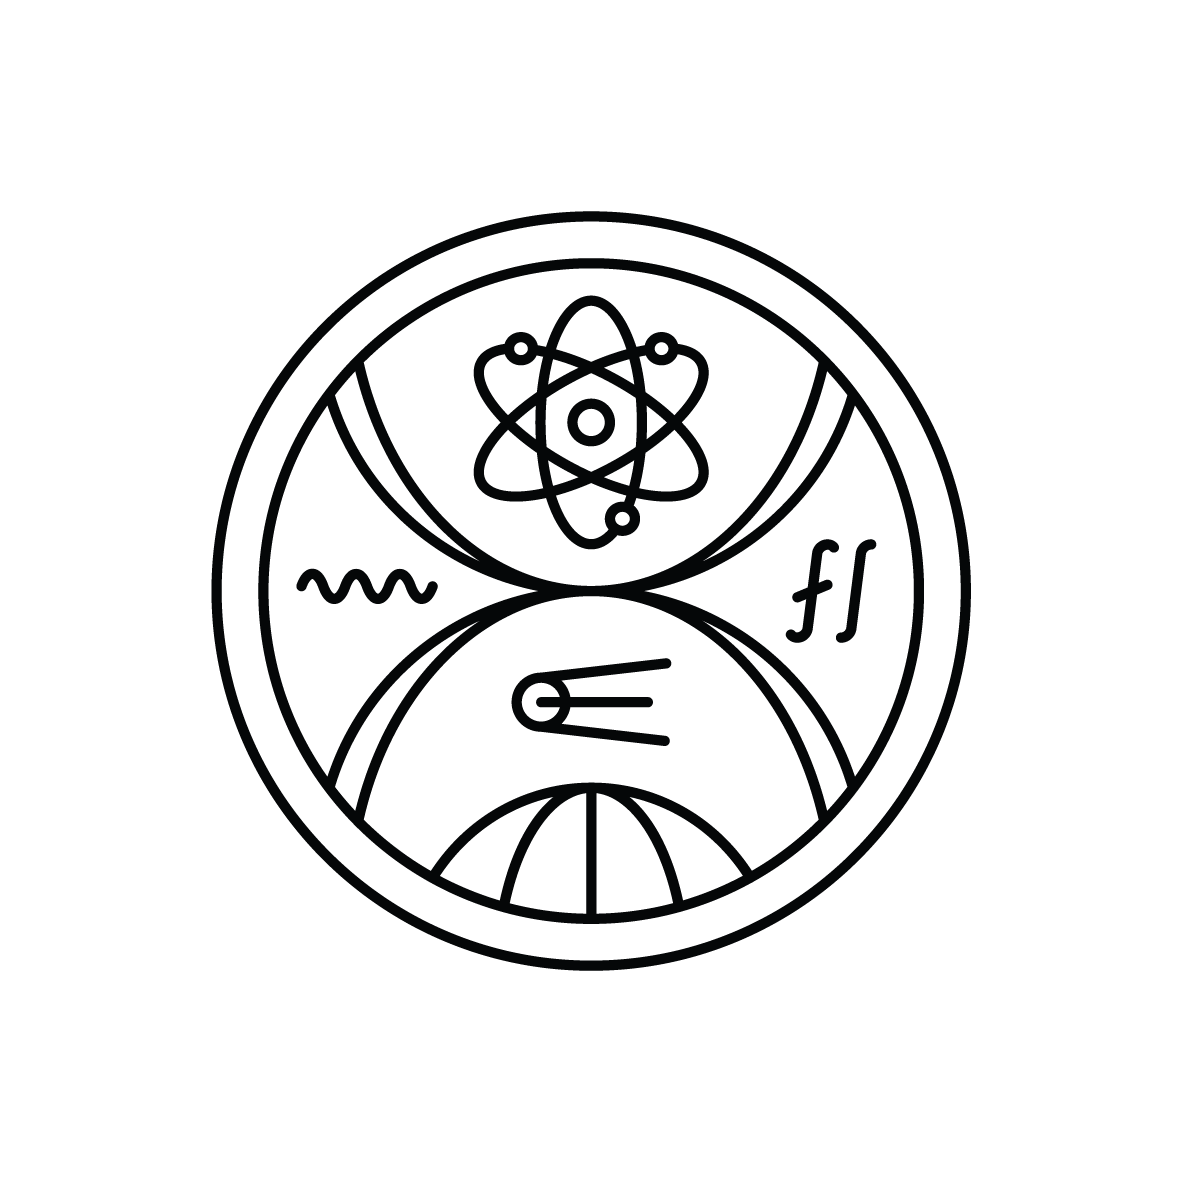
\includegraphics[width=0.4\textwidth]{images/FMFI_logo_BP.png}
		\label{img:logo}
	\end{center}
\end{figure}
\begin{center}
		\textbf{\MakeUppercase{\Large\mftitle}}\\
		\mfthesistype
\end{center}
\vfill
\mfrok \hfill
\mfauthor
%\eject 
\cleardoublepage
% --- koniec obalky ----



% -------------------
% --- Titulný list
% -------------------
\thispagestyle{empty}
\noindent
\begin{minipage}{\textwidth}
    \begin{center}
        \textbf{\mfuniversity \\
        \mffaculty}
    \end{center}
\end{minipage}

\vfill
\begin{figure}[!hbt]
    \begin{center}
        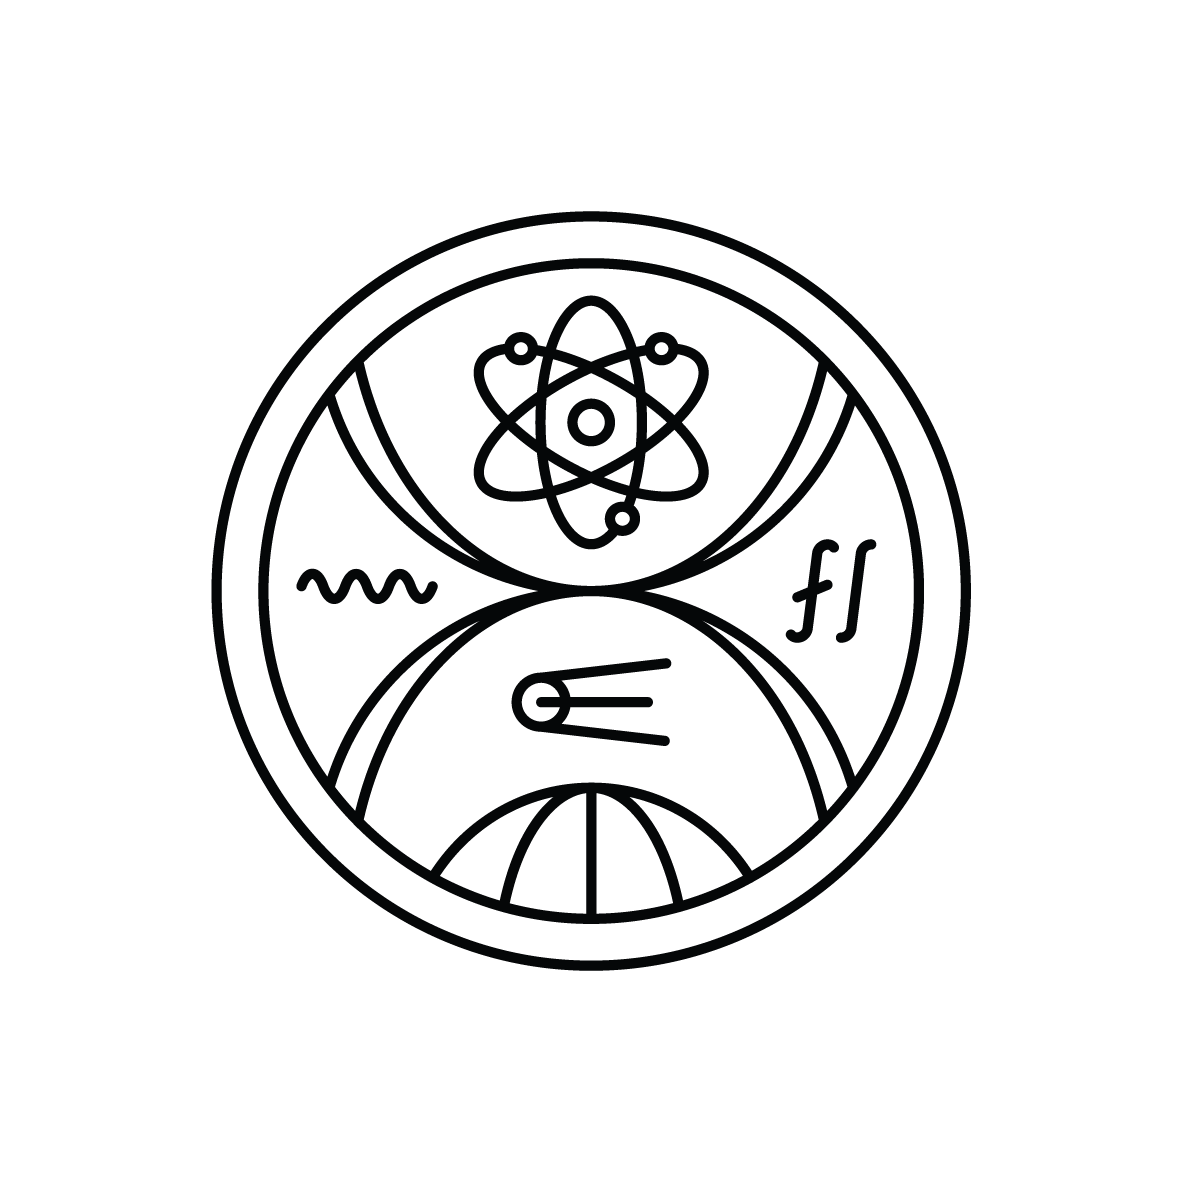
\includegraphics[width=0.4\textwidth]{images/FMFI_logo_BP.png}
        \label{img:logo_dark}
    \end{center}
\end{figure}

\begin{center}
	\textbf{\MakeUppercase{\Large\mftitle}}\\
	\mfthesistype
\end{center}
\vfill


\begin{tabular}{l l}
Study program: & \program \\
Branch of study: & \mfodbor \\
Department: & \mfpracovisko \\
Supervisor: & \mfskolitel \\
Consultant: & \mfkonzultant \\
\end{tabular}

\vfill
\noindent
\mfplacedate \hfill
\mfauthor
%\eject 
\cleardoublepage
% --- Koniec titulnej strany



% -------------------
% --- Zadanie z AIS
% -------------------
% v tlačenej verzii s podpismi zainteresovaných osôb.
% v elektronickej verzii sa zverejňuje zadanie bez podpisov
% v pracach v aglictine anglicke aj slovenske zadanie

\newpage 
\thispagestyle{empty}
\hspace{-2cm}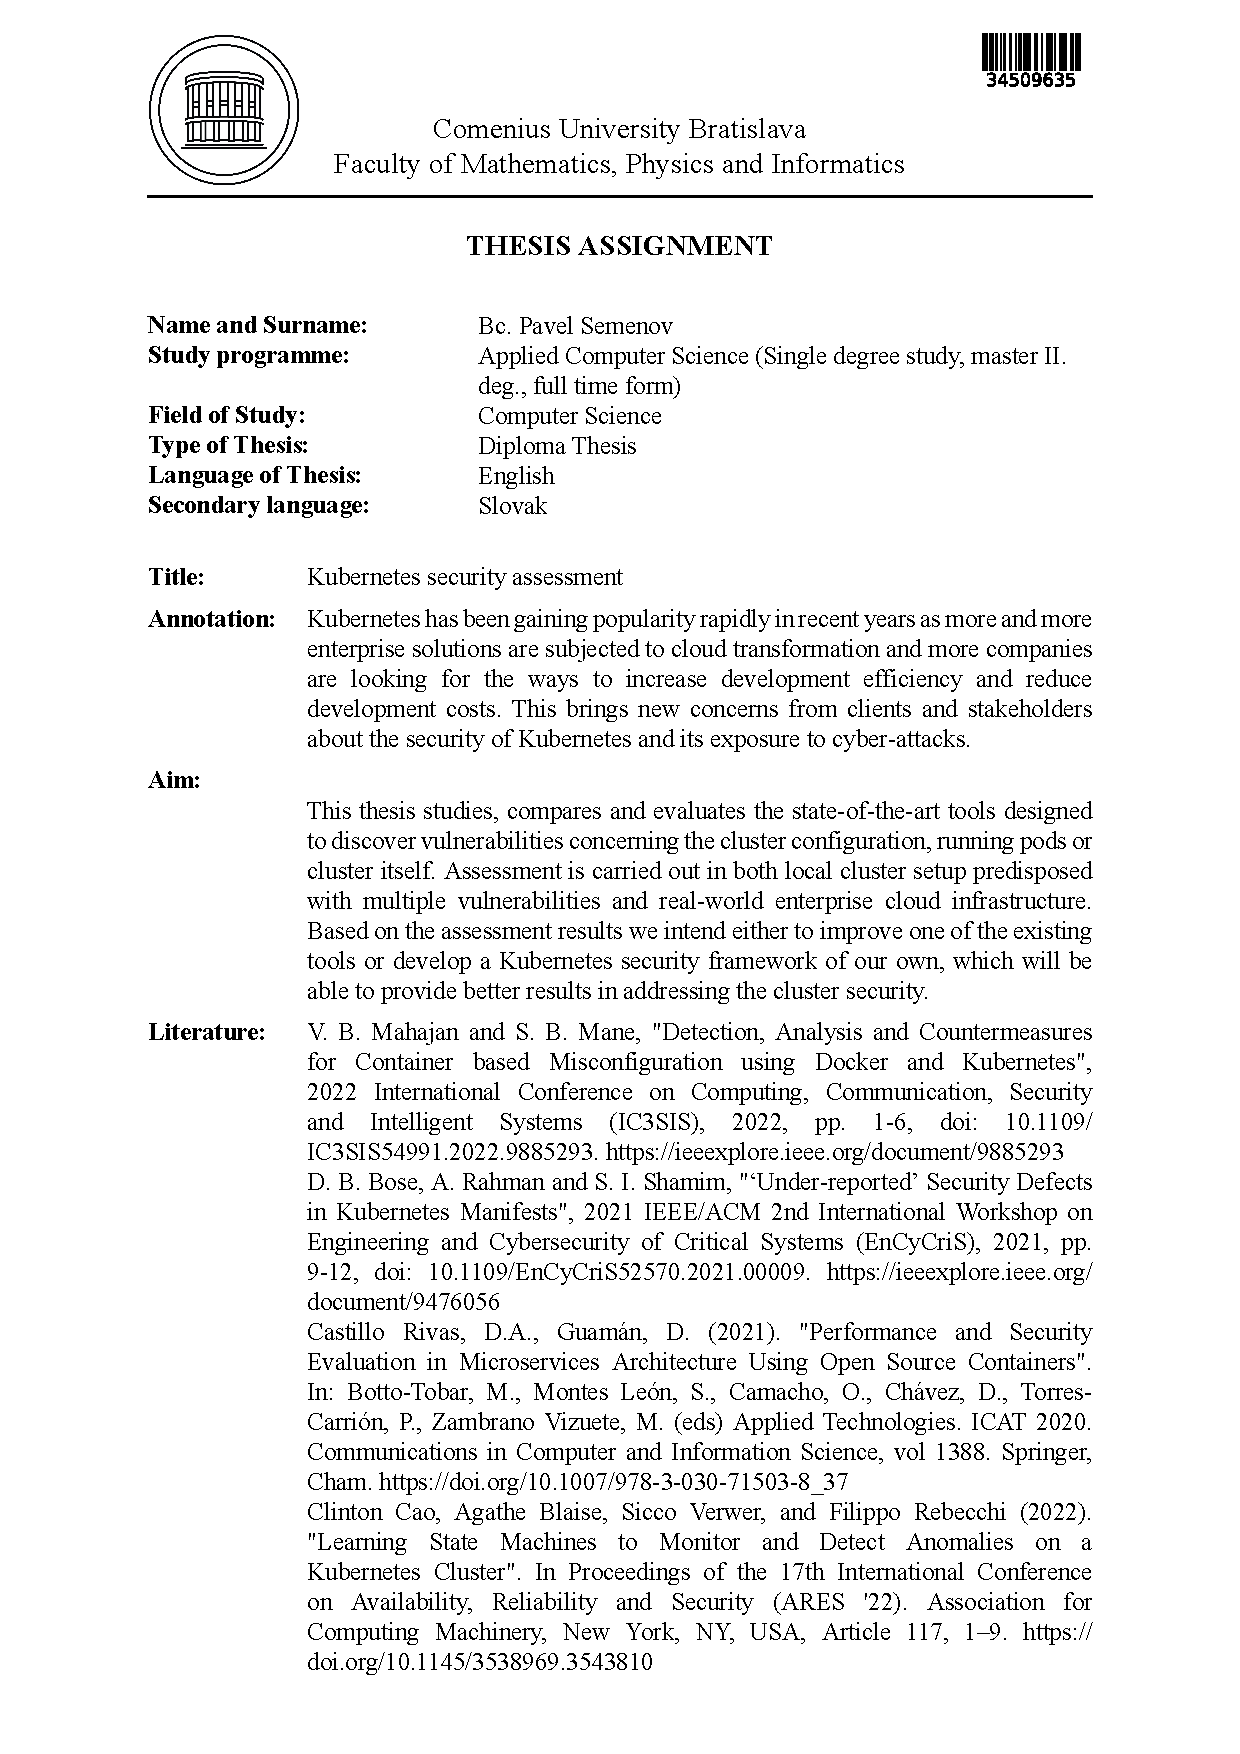
\includegraphics[page=1,width=1.1\textwidth]{assignment_en.PDF}

\newpage 
\thispagestyle{empty}
\hspace{-2cm}\includegraphics[page=2,width=1.1\textwidth]{assignment_sk.PDF}

% --- Koniec zadania


% -------------------
% --- Prehlásenie
% -------------------

{~}\vspace{12cm}

\noindent
\begin{minipage}{0.25\textwidth}~\end{minipage}
\thispagestyle{empty}
\begin{minipage}{0.75\textwidth}
I hereby declare that I have written this thesis by myself, only with help of referenced literature, under the careful supervision of my thesis advisor.
\newline \newline
\end{minipage}
\vfill
~ \hfill {\hbox to 6cm{\dotfill}} \\
\mfplacedate \hfill \mfauthor
\vfill\eject \cleardoublepage
% --- koniec prehlasenia




% -------------------
% --- Poďakovanie
% -------------------
\newpage
\thispagestyle{empty}
\chapter*{Acknowledgement}\label{chap:thank_you}
First, I would like to express my gratitude to Mgr. Ľubomír Firment for his guidance during the whole thesis and invaluable expertise in Kubernetes that made this thesis possible. I'd also like to thank my supervisor prof. RNDr. Richard Ostertág, PhD. for his insightful feedback.


\vfill\eject 
% --- koniec podakovania



% -------------------
% --- Abstrakty
% -------------------
\newpage 
\thispagestyle{empty}
\chapter*{Abstract}\label{chap:abstract_en}
Kubernetes has been gaining popularity rapidly in recent years as more and more enterprise solutions are subjected to cloud transformation and more companies are looking for the ways to increase development efficiency and reduce development costs. This brings new concerns from clients and stakeholders about the security of Kubernetes and its exposure to cyber-attacks.
This thesis studies, compares and evaluates the state-of-the-art tools designed to discover vulnerabilities concerning the cluster configuration, running pods or cluster itself. Assessment is carried out in both local cluster setup predisposed with multiple vulnerabilities and real-world enterprise cloud infrastructure. Based on the assessment results we intend either to improve one of the existing tools or develop a Kubernetes security framework of our own, which will be able to provide better results in addressing the cluster security.

\paragraph*{Keywords: kubernetes, security, test, cloud}  


\newpage 
\thispagestyle{empty}
\chapter*{Abstrakt}\label{chap:abstract_sk}
Zvýšený záujem o vesmírne aktivity spôsobil vznik vesmírneho odpadu obiehajúceho okolo Zeme. V posledných rokoch však vesmírny odpad predstavuje veľmi nebezpečný problém, ktorý môže ľahko ohroziť budúce vesmírne misie. Aby sa predišlo tomuto problému, je nevyhnutné pravidelné sledovanie a detekcia vesmírneho odpadu. Snímky získané z astronomických pozorovaní vesmírneho odpadu je potrebné spracovať a analyzovať, aby sme identifikovali astronomické objekty. Snímky zachytávajú signály z rôznych zdrojov. Od šumu spôsobeného nedokonalosťami CCD čipu, cez defekty spôsobené vonkajšími zdrojmi, alebo pozadím oblohy až po skutočné astronomické objekty, ako sú hviezdy, galaxie alebo objekty slnečnej sústavy (vesmírny odpad, satelity, kométy atď.)
Na správnu identifikáciu objektov, je potrebné obrázky najskôr očistiť od nežiadúcich efektov alebo navrhovaný algoritmus musí byť dostatočne robustný, aby sa zameral iba na signály zo skutočných astronomických objektov.

Na základe rozsiahleho výskumu analyzujúceho rôzne existujúce riešenia sme sa rozhodli použiť konvolučnú neurónovú sieť na vyriešenie úlohy klasifikácie vesmírnych objektov. V našej práci sme navrhli architektúru siete a prešli rozsiahlym procesom ladenia hyperparametrov. Aby sme sieť natrénovali a zároveň zabezpečili, že dáta sú robustné a vyvážené, generujeme syntetické snímky pomocou nášho vlastného generátora dát - starGen. Výkonnosť nášho modelu je vyhodnotená na reálnych dátach získaných z Astronomického a Geofyzikálneho observatória v Modre. Na zlepšenie výkonu tiež používame malé množstvo reálnych dát v kombinácii s technikami augmentácie na doladenie nášho modelu. V záverečnej časti porovnávame výkon nášho modelu s najmodernejšou sieťou ResNet-18.


\paragraph*{Kľúčové slová: kubernetes, bezpečnosť, testovanie, cloud}


% --- koniec abstraktov


% -------------------
% --- Obsah
% -------------------
\newpage 
\tableofcontents

% ---  Koniec Obsahu


% -------------------
% --- Zoznamy tabuliek, obrázkov - nepovinne
% -------------------
\newpage 
\listoffigures
\listoftables
% ---  Koniec Zoznamov

\chapter*{Terminology}

\section*{Terms}

\begin{itemize}
    \setlength\itemsep{1px}
    \item \textbf{CI/CD pipeline} \\
    CI/CD pipeline is a set of automatic tasks to be executed upon specific action resulting in ether failure on some of the pipeline stages or successful application deployment on the target environment. The aforementioned action might be a push into the source code repository or a manual pipeline run request. CI/CD pipeline usually includes build, test and deploy stages.
    \setlength\itemsep{1px}
    \item \textbf{Cloud} \\
    Term "Cloud" is ususally used to describe an array of (remote, on-premise or hybrid) servers that operate as a single ecosystem used for various hosting services.
    \item \textbf{Cloud provider} \\
    A cloud provider is a company that offers cloud computing services, which include resources like storage, processing power, networking, databases, and software, delivered over the internet.
\end{itemize}

\section*{Abbreviations}

\begin{itemize}
    \setlength\itemsep{1px}
    \item \textbf{K8s} - Kubernetes.
    \item \textbf{OS} - Operating System.
    \item \textbf{VM} - Virtual Machine.
    \item \textbf{CI/CD} - Continuous Integration/Continuous Deployment.
    \item \textbf{RBAC} - Role Based Access Control.
    \item \textbf{AWS} - Amazon Web Services.
    \item \textbf{TLS} - Transport Layer Security.
    \item \textbf{CSRF} - Cross Site Request Forgery.
    \item \textbf{XSS} - Cross Site Scripting.
    \item \textbf{OWASP} - The Open Worldwide Application Security Project.
    \item \textbf{TCP} - Transmission Control Protocol.
    \item \textbf{API} - Application Programming Interface.
    \item \textbf{NFS} - Network File System.
    \item \textbf{iSCSI} - Internet Small Computer Systems Interface.
\end{itemize}






\mainmatter

\chapter*{Motivation}
% spomenut vysledky  v clanku 
% preco sme sa rozhodli spravit tuto pracu

With a current upward trend in rocket launches and deployment missions, the population of resident space objects has increased rapidly. Due to the imperfections of our technology, we are unable to launch satellites into orbit without leaving behind fragments, rocket bodies and payloads, which gives a rise to the space debris environment. Moreover, more than 30 \% of satellites orbiting Earth are no longer functioning \cite{ESAarticle3}. As the space debris population is rising, the need for regular monitoring is essential. The detection of debris allows us to predict its position and actively avoid collisions. It may also help in future missions that aim to collect space debris. 

While many solutions to space object detection were already proposed, the majority of them focus on analytical methods. However, the immense amount of data acquired from the space observations, calls for an automatic and more robust technique - machine learning. 

In our thesis, we focus on the recognition of astronomical objects with unique features such as streaks, diffuse sources and contaminations on the CCD image. 
For this purpose, we have designed a convolutional neural network, that classifies images based on the astronomical objects present in them. To train our network with a sufficient amount of data we have implemented a data simulator that generates synthetic astronomical images. The results of our thesis have also been published in the article \cite{soi2022} and presented at the 3rd IAA Conference on Space Situational Awareness.  


%The proposed system is our own convolutional neural network, that extracts features from the images and classifies them based on the object 

%With this in mind, we propose a convolutional neural network to solve this task 

%In recent years, the machine learning methods have spiked the interest in computer vision and the astronomical field is no exception. 
\chapter{Introduction}

\section{Containerization}

When talking about the Kubernetes it is essential to be familiar with the technology of containerization. This chapter introduces the reader to the basics of the containerization. We start by giving a short definition, then we examine core concepts of the containerization such as container image and Docker. Then we compare it to the traditional means of application deployment. Finally, we examine the security on the container image level.

\subsection{Overview}

According to IBM, containerization is the packaging of software code with just the operating system libraries and dependencies required to run the code to create a single lightweight executable—called a container—that runs consistently on any infrastructure. \cite{ibm-containerization}.

Although containers are built to be infrastructure-agnostic, there are still certain compatibility considerations to keep in mind. One significant factor is processor architecture. Containers built for a specific architecture family (e.g., arm64, amd64, or x86) are generally not cross-compatible with infrastructures based on different architectures. However, it is possible to build multi-architecture containers that support multiple processor architectures in a single image, enhancing the flexibility and portability of the containerized applications across diverse environments.

\subsection{Container Image}

Container images are software application packages, which are shipped with all required libraries, binaries and configurations. In another words, container images are lightweight and higly portable artifacts. Usually container images are stored in Container Registries, either public (e.g. Dockerhub) or private. When an image transitions into the running state, it becomes a container.

Container images are comprised of multiple layers. At the base layer there is usually some lightweight Linux distribution. Then, each layer introduce a change in the environment, a change might be in the code or binary, runtimes, dependencies, and other filesystem objects required to run an application.

\subsection{Docker}

Docker is the most widely used containerization tool. It ships tools to build, run and store containers. Docker Engine is a collective name for the Docker build toolkit. First, there is a \lstinline{dockerd} or Docker Daemon, which is a server running in the backend. Secondly, the user intercts with Docker CLI or Docker Client to build and run images. Docker Clients communicates with Docker Daemon through the Rest API served at the backend. Then, there is Docker Compose, which a simple orchestration tool for the containers. It can be used to compose a few containers into a system with a shared network and storage. Lastly, Dockerhub is a public container registry, where the bulk of the publicly available images are stored.

Images are built based on the Dockerfile, which is a set of instructions. Each instruction introduces a new layer to the image. Layers can then be smartly reused by the Docker Engine to build different images with similar bases. Listing~\ref{lst:dockerfile} demonstates an example of the Dockerfile. Each Dockerfile starts with a \lstinline{FROM} command, which specifies the base image to use for this container. The \lstinline{FROM} keyword is followed by the base image name. In our case, \lstinline{registry.redhat.io} is the registry address. It is followed by the repository name (\lstinline{ubi8} in our case), which is separated from the registry name by a single slash and may be preceeded by the namespace. Lastly, tag follows repository name and separated with a colon from it. Both registry address and tag are optional. In case registry name is omitted, Docker will search for the image in the Dockerhub. If the tag is not provided, Docker will fetch \lstinline{latest} tag.

\begin{lstlisting}[language=Dockerfile, caption={A simple Dockerfile for a NodeJS app.}, label={lst:dockerfile}]
    FROM registry.redhat.io/ubi8:latest
    RUN dnf install nodejs && \
        useradd -u 1000 -g 1000 -M node
    COPY --chown=node:node src /app
    WORKDIR /app/src
    USER node
    RUN npm ci
    EXPOSE 3000
    ENTRYPOINT ["npm", "run"]
\end{lstlisting}

\lstinline{RUN} command is used to run commands inside the container during the build phase. All artefacts generated by the \lstinline{RUN} command stay inside the contaier and can be used during runtime. In our case we are installing the necessary binaries to run our application and creating a user to run the application. \lstinline{COPY} command copies the specified resource from the local machine into the container. We also are changing the ownership for the copied files. \lstinline{WORKDIR} command affects the commands after it, so that they are executed from the specified directory. \lstinline{USER} command changes the current user. Last \lstinline{USER} command inside the Dockerfile determines under which user the main process inside the container is running in the runtime. In our case we use our newly created \lstinline{node} user. The default user for the container is \lstinline{root}. \lstinline{EXPOSE} command ensures that a specific port on the container is open for the external communication. Lastly, \lstinline{ENTRYPOINT} is one of the few ways to define the main process of the container. When main process ends, the container stops.

\subsection{Containerization vs Virtualization}

Let us discuss why containerization is the internationally accepted enterprise solution nowadays and why do software arhitects tend to choose it over traditional virtualization solutions.

Figure~\ref{img:containers-vs-virtual-machines} provides a side-by-side comparison of a Virutal Machine and a Cloud infrastructure, each with three applications deployed. We can see that each application on the container side is missing a "Guest OS" layer. Here lies the main advantage of the containers. Absence of the Guest Operating System provides a lot of advantages, which we discuss further below.

\begin{figure}[!hbt]
	\begin{center}
		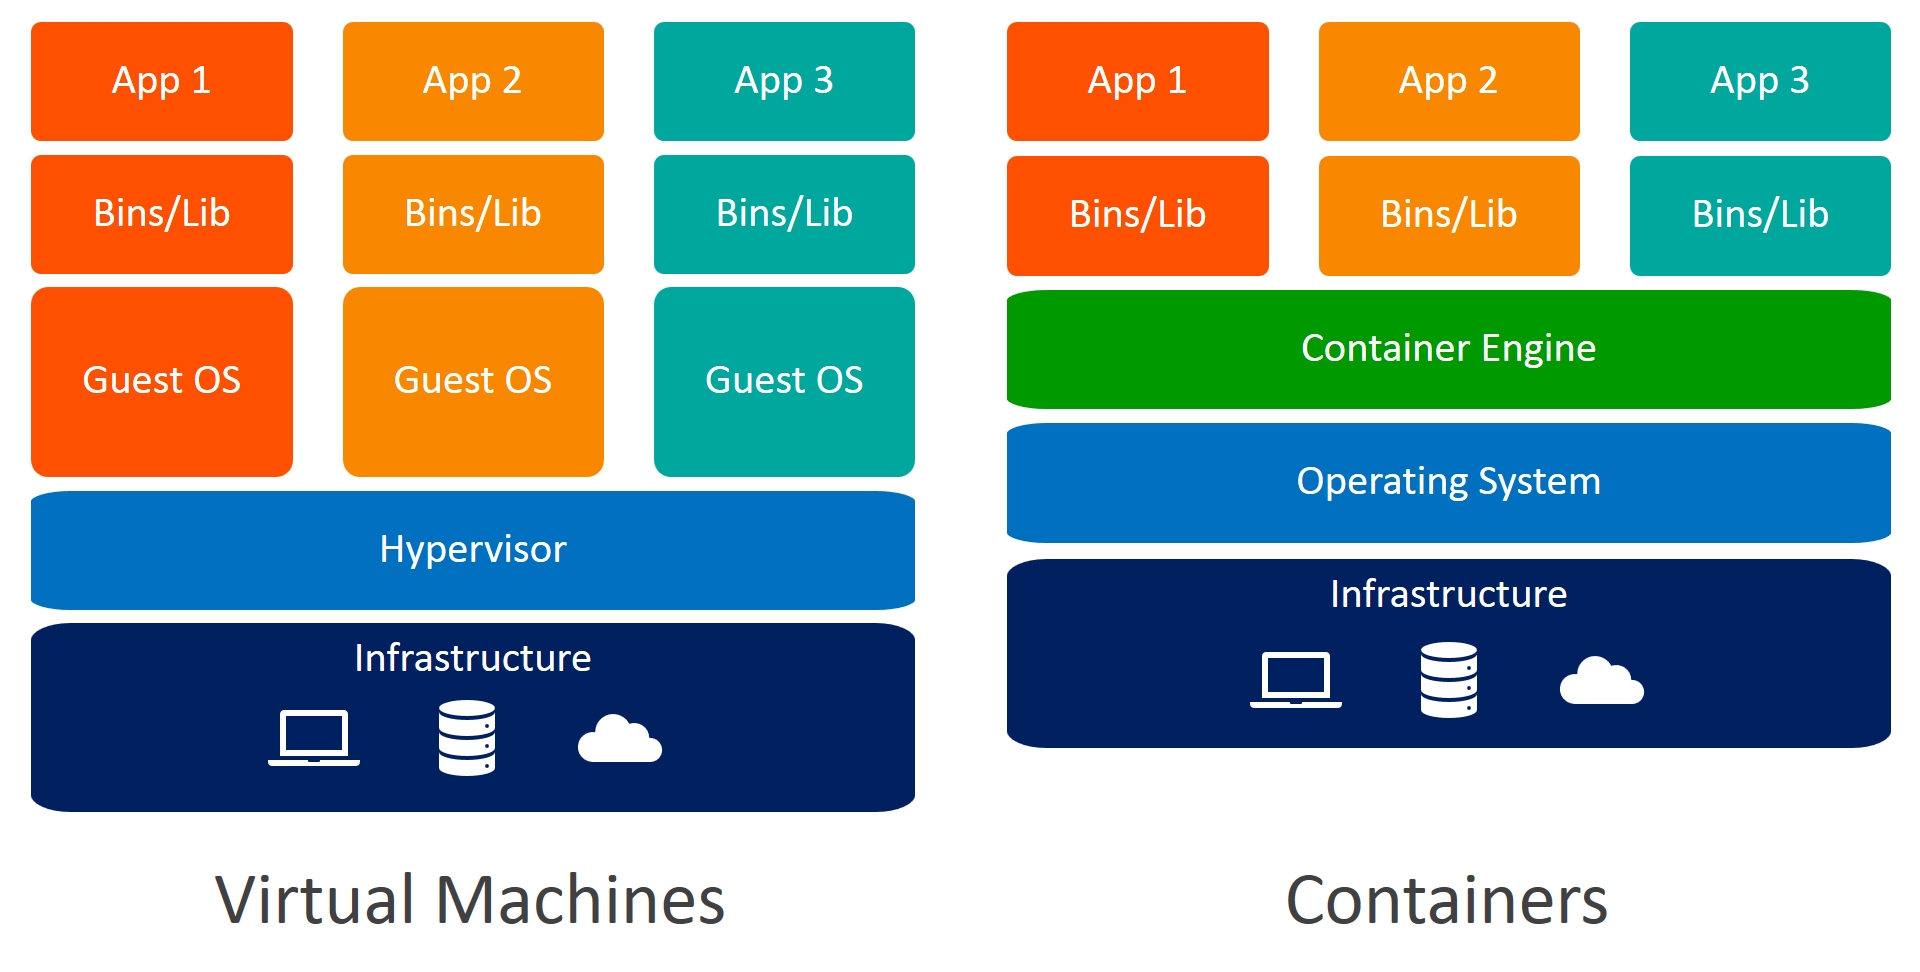
\includegraphics[width=0.75\textwidth]{images/containers-vs-virtual-machines.jpg}
        \caption{Side-by-side comparison of VM and container infrastructures.}
		\label{img:containers-vs-virtual-machines}
	\end{center}
\end{figure}

The most important advantage of the containers is their resource efficiency. Containers only include the application code and its dependencies, which makes them very small compared to the Virtual Machines, which tend to be very bulky and grow in size as development progresses. Containers share the host operating system kernel, so they consume significantly less CPU, memory, and storage than virtual machines, which require a full OS for each instance. This lightweight nature allows more containers to run on a single host, maximizing resource utilization and reducing overhead. Better resource efficiency means also lower costs for the user.

Then, startup speeds are significantly lower for the containers as they do not need to initialize the whole OS boot sequence. This feature also enables the scaling capabilities for the containers, allowing applications to respond quickly to changes in demand.

Additionally, the containers are more consistent than virtual machines. Packed with the required dependencies, they behave in the same way across different environments. As they are isolated from the OS, containers are almost immune to the compatibility issues. This gives them a strong portability advantage. They provide an abstraction that makes it easier to move workloads across various platforms.

Lastly, containers also lead when it comes to automation and CI/CD pipelines. Containers can be easily versioned, updated, and rolled back, allowing for smooth integration into CI/CD pipelines. This streamlines deployment, testing, and rollback processes, leading to faster development cycles. VMs can also be updated and rolled back, but the process is usually slower and more complex.

These are some of the most significant advantages of containerization. All of them contribute to fast build and deploy speeds, which also means high development speeds. While costing less money and providing a lot more flexibility, they become essential for successful enterprise software development. For large-scale development, test and production environment containerization has become an obvious choice over the virtualization.

\subsection{Security Concepts}
\section{Kubernetes}

In this section we will dive into the topic of Kubernetes. We start by shortly overviewing the Kubernetes architecure. Then we expand on the Kubernetes resources, their kinds and their role in the target application environment. Finally, we consider the security of Kubernetes.

\subsection{Overview}

Kubernetes, also known as K8s, is an open source system for automating deployment, scaling, and management of containerized applications. It groups containers that make up an application into logical units for easy management and discovery. Kubernetes builds upon 15 years of experience of running production workloads at Google, combined with best-of-breed ideas and practices from the community. \cite{kubernetes}.

IBM defines Kubernetes as an open source \textbf{container orchestration platform} for scheduling and automating the deployment, management and scaling of containerized applications. Today, Kubernetes and the broader ecosystem of container-related technologies have merged to form the building blocks of modern cloud infrastructure. This ecosystem enables organizations to deliver a highly productive hybrid multicloud computing environment to perform complex tasks surrounding infrastructure and operations. It also supports cloud-native development by enabling a build-once-and-deploy-anywhere approach to building applications. \cite{ibm-kubernetes}.

It is important to emphasize that the Kubernetes abstracts the actual machines (nodes) from the user. Nodes can be physical on-premises servers, or VMs that reside either on-premises or at a cloud provider. Kubernetes takes on the responsibilty of figuring out the deployment target for a particular application. That is, user only defines the desired state of the infrastructure using YAML or JSON configuration files. Kubernetes then creates all the workloads based on the applied configuration.

\subsection{Kubernetes Architecture}

While Kubernetes requires at least three nodes to run, there are some implementation designed for the local use, which emulate this concept (see Subsection~\ref{sec:other-kubernetes-implementations}). The master node is called control plane. The control plane manages the worker nodes and the Pods in the cluster. In production environments, the control plane usually runs across multiple computers and a cluster usually runs multiple nodes, providing fault-tolerance and high availability. Worker nodes host the actual workload inside the cluster. Figure~\ref{img:kubernetes-architecture} provides a simple high-level overview of a typical Kubernetes cluster with a Control Plane and three worker nodes.

\begin{figure}[!hbt]
	\begin{center}
		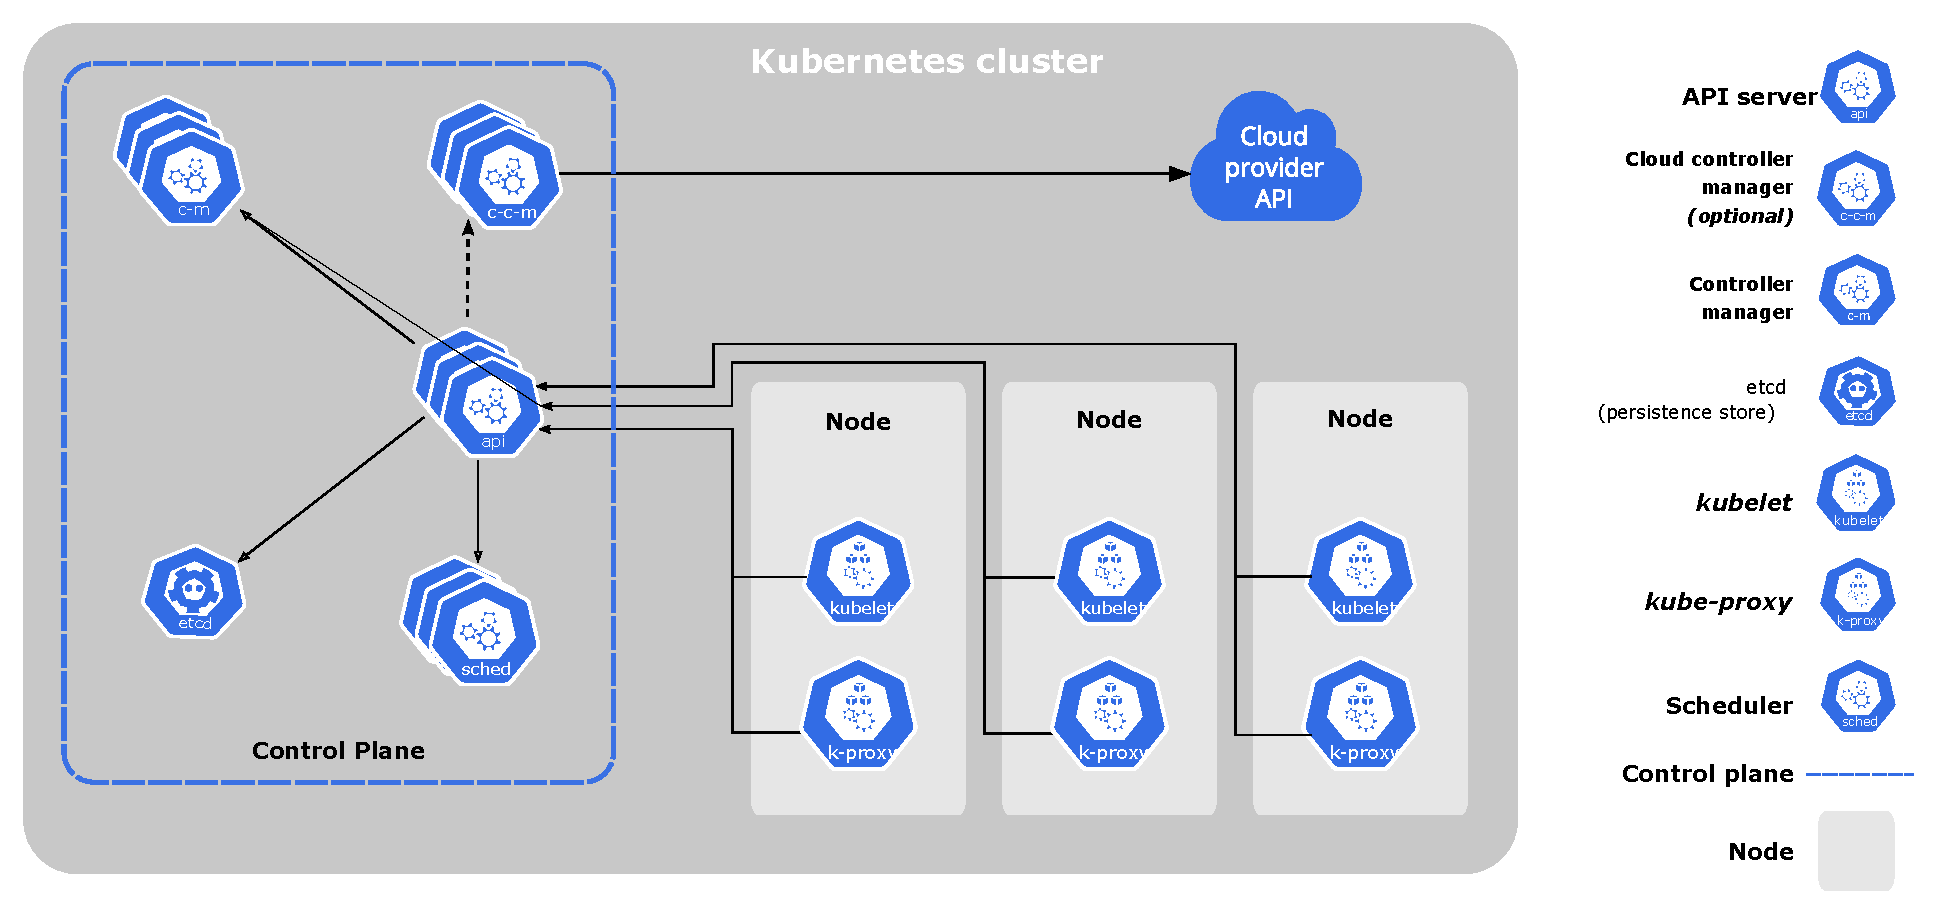
\includegraphics[width=0.85\textwidth]{images/components-of-kubernetes.pdf}
        \caption{Kubernetes cluster architecure overview with its main components.}
		\label{img:kubernetes-architecture}
	\end{center}
\end{figure}

\subsubsection*{Control Plane overview}

Control plane runs the following components: 
\begin{itemize}
\item \textbf{kube-apiserver} \\
Kube-apiserver exposes the Kubernetes API, which is acting as a frontend for the Kubernetes control plane.
\item \textbf{etcd} \\
Etcd is a key-value store, where all of the cluster data is stored.
\item \textbf{kube-scheduler} \\
Each time a new pod is created, it is passed to the kube-scheduler, which assigns the pod to the specific node to run on (based on individual and collective resource requirements, hardware/software/policy constraints, affinity and anti-affinity specifications, data locality, inter-workload interference, and deadlines).
\item \textbf{kube-controller-manager} \\
Each Kubernetes resource has its own controller (e.g. NodeController, JobController, ServiceAccountController); all of them are compiled as one binary called kube-controller-manager.
\item \textbf{cloud-controller-manager} \\
Cloud-controller-manager embeds cloud-specific control logic. It differs depending on the cloud provider or can be absent completely, when running Kubernetes locally.
\end{itemize}

\subsubsection*{Worker Node overview}

Each worker node has a kubelet and kube-proxy installed. Kubelet is an agent that manages runnning pods and containers. Kube-proxy is a network proxy that implements parts of the Kubernetes service concept. It maintains network rules on nodes, making in- outside-cluster communitcation possible.

Then, of course, each worker node has a set of running pods. A typical use would involve multiple running applications. Depending on the size of the node and the application resoucre consumption it can accomodate on average from one to a few dozens applications with various business purposes.

\subsection{Kubernetes Resources}

Kubernetes resources are fundamental components that define various entities within a Kubernetes cluster. Resources are objects that represent the desired state and configuration of the infrastructure, applications, and services running on the cluster. Kubernetes provides a range of resources that enable developers and operators to define, manage, and scale containerized applications, network policies, storage requirements, and more. These resources are defined declaratively in YAML or JSON files, which makes infrastructure setup consistent and reproducible.

Among key Kubernetes resoucres are:
\begin{itemize}
    \item \textbf{Pods} \\
        Pod is the atomic workload unit in the Kubernetes cluster. It encapsulates one or more containers that share the same network. It represents a single instance of a running application.
    \item \textbf{Deployments} \\
        Deployments are a higher level of abstraction for the Pods. They allow to define replica count and rollout/rollback strategy for the updates, which can be used to ensure availability for the application.
    \item \textbf{Services} \\
        Services provide a communication layer for the pods inside one cluster. Being an abstraction over the pods' network, they provide reliable access to the selected workloads, while serving as a Load Balancer. 
    \item \textbf{ConfigMaps} and \textbf{Secrets} \\
        ConfigMaps and Secrets allow users to store data outside the workload. ConfigMaps are usually used to store non-sensitive information like environment and application configuration parameters. Secrets are a more secure resource designed for API keys, passwords and other sensitive data.
    \item \textbf{PersistentVolumes} and \textbf{PersistentVolumeClaims} \\
        These resources enable stateful applications to request and mount durable storage within a cluster, allowing data to persist independently of the Pod lifecycle.
\end{itemize}

Above are the most commonly used resources, which we also leverage in the practical part of the paper. Therefore, it is important that the reader understands the position and the purpose of each resource in the cluster infrastructure.

\subsubsection*{Workloads}

Minimal computing units in Kubernetes are Containers, which are running in Pods. However, to simplify the management of Pods, Kubernetes has workload resources, which manage the set of Pods. They make sure the desired number of Pods of right kind are running to match the declaration.

Deployments and ReplicaSets are a good fit for stateless applications. Each pod in the Deployment is interchangebeable. Deployments are easily scalable and have built-in versioning and rollout mechanisms.

StatefulSet allows to create sets of stateful applications. They might share the same PersistentVolume and replicate data between each other.

DaemonSet defines Pods that provide node-local facilities. These might be fundamental to the operation of your cluster, such as a networking helper tool, or be part of an add-on.

Job and CronJob define tasks that run to completion and then stop. Jobs represent one-off tasks, whereas CronJobs recur according to a schedule.

\subsubsection*{Networking}

Kubernetes networking model makes Pods look like VMs in the networking aspect. Pods on any nodes can communicate with each other without NAT. Containers inside the same Pod share its network meaning that they can reach each other using localhost.

Kubernetes networking addresses four concerns:
\begin{itemize}
\item Containers within a Pod use networking to communicate via loopback.
\item Cluster networking provides communication between different Pods.
\item The Service API lets you expose an application running in Pods to be reachable from outside your cluster.
\item Ingress provides extra functionality specifically for exposing HTTP applications, websites and APIs.
\item You can also use Services to publish services only for consumption inside your cluster.
\end{itemize}

\subsubsection*{Storage}

Kubernetes does not ship a particular implementation of storage. However, it provides a range of resources that define the storage concept and supports different types of volumes. A Pod can use any number of volume types simultaneously. Ephemeral volume types have a lifetime of a pod, but persistent volumes exist beyond the lifetime of a pod. When a pod ceases to exist, Kubernetes destroys ephemeral volumes; however, Kubernetes does not destroy persistent volumes. For any kind of volume in a given pod, data is preserved across container restarts.

At its core, a volume is a directory, possibly with some data in it, which is accessible to the containers in a pod. How that directory comes to be, the medium that backs it, and the contents of it are determined by the particular volume type used.

PersistentVolumes and PersistentVolumeClaims are the resources kinds most important to understand here.
\begin{itemize}
\item A PersistentVolume (PV) is a piece of storage in the cluster that has been provisioned by an administrator or dynamically provisioned using Storage Classes. It is a resource in the cluster just like a node is a cluster resource. PVs are volume plugins like Volumes, but have a lifecycle independent of any individual Pod that uses the PV. This API object captures the details of the implementation of the storage, be that NFS, iSCSI, or a cloud-provider-specific storage system.
\item A PersistentVolumeClaim (PVC) is a request for storage by a user. It is similar to a Pod. Pods consume node resources and PVCs consume PV resources. Pods can request specific levels of resources (CPU and Memory). Claims can request specific size and access modes (e.g., they can be mounted ReadWriteOnce, ReadOnlyMany or ReadWriteMany). Once and Many here refer to a number of Pods that can perform the read or write simultaneously.
\end{itemize}

\subsection{Infrastructure Security}

When we are talking about the infrastructure security, we must consider multiple layers. Going from the top to the bottom, we start with the security measurements taken on the Cloud provider side. In most cases this is not something we can affect and the security of different Cloud providers varies significantly. Unfortunately, this is out of scope of this paper, but all of the "big five" Cloud providers (AWS, Azure, Google Cloud, Alibaba and IBM) maintain high security standarts and security risks generally should not be a concern for their end users. Then, we get to the cluster itself. On the cluster level we must consider the security of the nodes, security of the cluster components and their configuration. At this layer we have already some space for the misconfigurations to appear. Here we can evaluate the security of the single components using some of the security scanners presented in \nameref{sec:kubernetes-security-automation}. Lastly, we get to the application level, where the security of the application code, Kubernetes resoucre configuration, libraries, dependencies and base images is the main concern. Again, this is the layer, where the developers have the most access to, thus, providing a lot of space for the possibility of a human error. In this paper we mostly work on this level when we do our research.

Officially, The Linux Foundation provides only some security guidelines for each of the layers. However, bundled with Kubernetes we get a few means to keep the security under control. Below we present an overview of the Kubernetes security recommendations, RBAC and Data security inside Kubernetes.

\subsubsection*{Kubernetes security recommendations}

This section gathers the official security recommendations provided by the Kubernetes. They provide a list of concerns for each level of the cloud infrastructure. Cloud infrastructure can be viewed as a composition of four layers as displayed by the Figure~\ref{img:cloud-security}.

\begin{figure}[!hbt]
	\begin{center}
		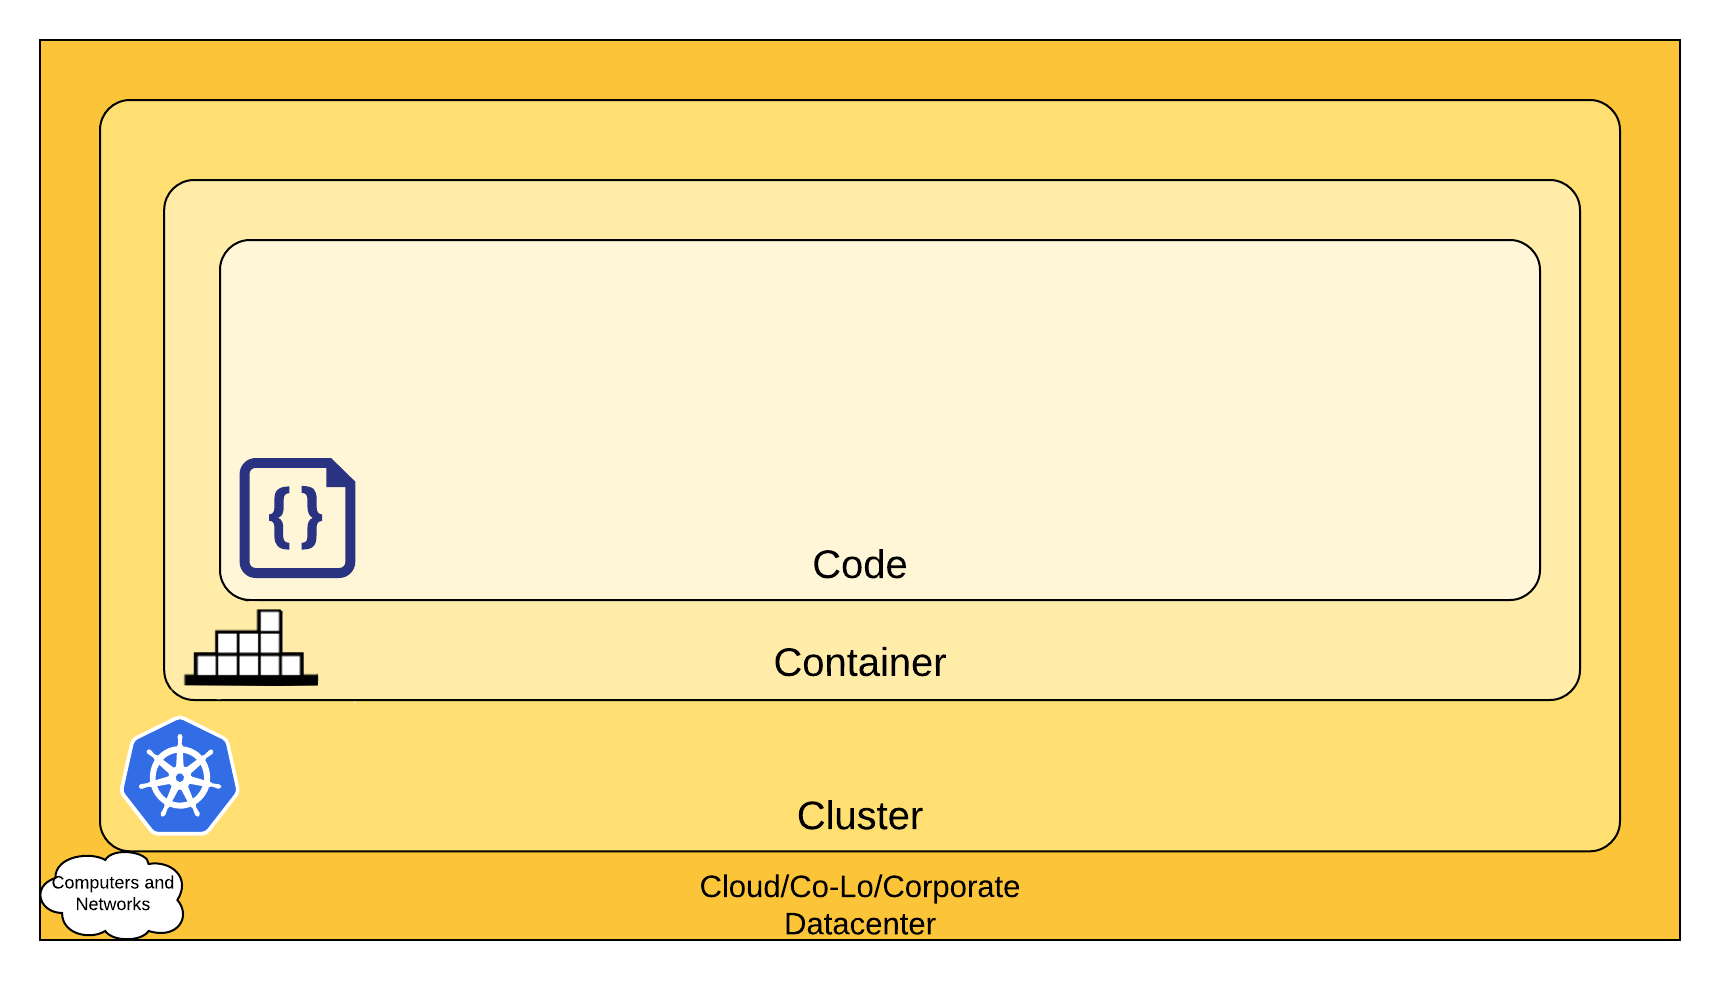
\includegraphics[width=0.75\textwidth]{images/cloud-security.png}
        \caption{Four layers of the cloud infrastructure.}
		\label{img:cloud-security}
	\end{center}
\end{figure}

Each layer is built upon the previous one and its security depends on the security of the outer layers. It is, therefore, important to maintain high security standarts on base levels (Cloud, Cluster, Container).

\begin{enumerate}

\item \textbf{Cloud} \\
Each cloud provider has its own security policies and guidelines. There are, however, some general infrastructure-level security best advice described by in the Table~\ref{tab:cloud-security-recommendations}.

\begin{table}[H]
    \begin{center}
        \begin{tabular}{ | p{.20\textwidth} | p{.80\textwidth} | } 
         \hline
         \textbf{Area of Concern for Kubernetes Infrastructure} & \textbf{Recommendation} \\ 
         \hline
         Network access to API Server (Control plane) & All access to the Kubernetes control plane is not allowed publicly on the internet and is controlled by network access control lists restricted to the set of IP addresses needed to administer the cluster. \\ 
         \hline
         Network access to Nodes (nodes)  & Nodes should be configured to only accept connections (via network access control lists) from the control plane on the specified ports, and accept connections for services in Kubernetes of type NodePort and LoadBalancer. If possible, these nodes should not be exposed on the public internet entirely. \\ 
         \hline
         Kubernetes access to Cloud Provider API & Each cloud provider needs to grant a different set of permissions to the Kubernetes control plane and nodes. It is best to provide the cluster with cloud provider access that follows the principle of least privilege for the resources it needs to administer. \\
         \hline
         Access to etcd & Access to etcd (the datastore of Kubernetes) should be limited to the control plane only. Depending on your configuration, you should attempt to use etcd over TLS. \\
         \hline
         etcd Encryption & Wherever possible it's a good practice to encrypt all storage at rest, and since etcd holds the state of the entire cluster (including Secrets) its disk should especially be encrypted at rest. \\
         \hline
        \end{tabular}
    \end{center}
    \caption{Security recommendations for the Cloud layer.}
    \label{tab:cloud-security-recommendations}
\end{table}

\item \textbf{Cluster} \\
There are two cluster security concerns that could be addressed: securing the configurable cluster components and securing the applications running in the cluster.

There are a few things to consider regarding the application security:
\begin{itemize}
\item RBAC Authorization (Access to the Kubernetes API)
\item Authentication	
\item Application secrets management (and encrypting them in etcd at rest)
\item Ensuring that pods meet defined Pod Security Standards
\item Quality of Service (and Cluster resource management)
\item Network Policies
\item TLS for Kubernetes Ingress
\end{itemize}

\item \textbf{Container} \\
Securing containers is a vast topic, which deserves its own chapter. There are, nevertheless, a few general recommendation provided by the Kubernetes, which you can find in the Table~\ref{tab:container-security-recommendations}.

\begin{table}[H]
    \begin{center}
        \begin{tabular}{ | p{.20\textwidth} | p{.80\textwidth} | } 
        \hline
        \textbf{Area of Concern for Containers} & \textbf{Recommendation} \\ 
        \hline
        Container Vulnerability Scanning and OS Dependency Security & As part of an image build step, you should scan your containers for known vulnerabilities. \\ 
        \hline
        Image Signing and Enforcement & Sign container images to maintain a system of trust for the content of your containers. \\ 
        \hline
        Disallow privileged users & When constructing containers, create users inside of the containers that have the least level of operating system privilege necessary in order to carry out the goal of the container. \\
        \hline
        \end{tabular}
    \end{center}
    \caption{Security recommendations for the Container layer.}
    \label{tab:container-security-recommendations}
\end{table}

\item \textbf{Code} \\
When it comes to code, the developers have the most flexibility to design secure applications. There are a lot of issues to address, which may vary significantly from application to application depending on its purpose, architecture and framework base. Kubernetes documentation gives a handful of recommendations regarding this topic, which are displayed below in the Table~\ref{tab:code-security-recommendations}.

\begin{table}[H]
    \begin{center}
        \begin{tabular}{ | p{.20\textwidth} | p{.80\textwidth} | } 
        \hline
        \textbf{Area of Concern for Code} & \textbf{Recommendation} \\ 
        \hline
        Access over TLS only & If your code needs to communicate by TCP, perform a TLS handshake with the client ahead of time. With the exception of a few cases, encrypt everything in transit. Going one step further, it's a good idea to encrypt network traffic between services. This can be done through a process known as mutual TLS authentication or mTLS which performs a two sided verification of communication between two certificate holding services. \\ 
        \hline
        Limiting port ranges of communication & This recommendation may be a bit self-explanatory, but wherever possible you should only expose the ports on your service that are absolutely essential for communication or metric gathering. \\ 
        \hline
        3rd Party Dependency Security & It is a good practice to regularly scan your application's third party libraries for known security vulnerabilities. Each programming language has a tool for performing this check automatically. \\
        \hline
        Static Code Analysis & Most languages provide a way for a snippet of code to be analyzed for any potentially unsafe coding practices. Whenever possible you should perform checks using automated tooling that can scan codebases for common security errors. \\
        \hline
        Dynamic probing attacks & There are a few automated tools that you can run against your service to try some of the well known service attacks. These include SQL injection, CSRF, and XSS. One of the most popular dynamic analysis tools is the OWASP Zed Attack proxy tool. \\
        \hline
        \end{tabular}
    \end{center}
    \caption{Security recommendations for the Code layer.}
    \label{tab:code-security-recommendations}
\end{table}
                      
\end{enumerate}

\subsubsection*{Role Based Access Control}

\subsubsection*{Data security}

\subsection{Other Kubernetes Implementations}
\label{sec:other-kubernetes-implementations}

\subsubsection*{Openshift}

\subsubsection*{Rancher Desktop}
%\section{Kubernetes security automation}
\label{sec:kubernetes-security-automation}

This section introduces the reader to the topic of the security automation inside the Kubernetes cluster. We discuss different security tools, their place in the cloud Infrastructure and examine their usage patterns. Additionally, we explain why were the specific tools chosen for our research.

\subsection{Overview}

Kubernetes security scanners and operators provide an array of defensive capabilties. Most of them act in the form of informator. That is, they do not perform any remediatory actions, but only provide user with information about the cluster security status. Nevertheless, there are some solutions on the market that are capable of resolving some of the security issues automatically. This, on the other hand, introduces another layer of concern: can we really trust a third-party system to introduce modifications to our infrastructure? That the former type is the most abundant and is the focus of this paper. Automatic remediation can be then implemented as a part of CI/CD pipeline based on the scan results. This ensures that it is compliant with the company's policies and is tailored to the company's needs.

One of the ways to classify Kubernetes security scanners is by the scan target. Here we can roughly divide them into three groups: configuration file scanners, cluster scanners and container image scanners. Most of the tools, however, can be put into multiple different groups. Cluster scanners usually are able to perform container image scanning as well and it is a part of the full cluster scan. Cluster scanners detect misconfigurations in the cluster infrastructure and its essential components. They look for, among other things, containers running with extensive privilages, exposed sensitive workloads and plaintext secrets. Container image scanners look for known vulnerabilities inside the images. Configuration file scanners perform a scan of the cluster configuration files. For large infrastructure with a number of applications deployed there might be over several tens of thousands lines of configuration and such scanners aim to detect any known misconfigurations by going through theese lines.

Cluster security scanners can be further classified by the execution point. Again, there is usually more than one way to run a scan, but here are a few options: run a scanner tool as a container, run it from a remote machine connected to the cluster, run it is an operator, which can perform scan automatically on a regular basis. To always keep cluster up-to-date with the most recent security patches the best solution would be to either install an operator or integrate a security scanner tool into your CI/CD pipeline.

\subsection{Selection Criteria}

To perform our assessment we have chosen from a variety of Kubernetes security scanners. Though the area is still relatively new, there is a variety of tools with different purposes available on the market. We made our choice based on the following criteria:
\begin{itemize}
\item \textbf{free-to-use} \\
We do include some proprietary tool testing further in our research as an additional comparison, however, for the main part we only use free tools. Kubernetes itself is distributed under Apache License 2.0, which means it is inherently free to use. The ability to adopt these tools without financial constraints enables wider adoption, thus, contributing to the community-driven innovations. Finally, this research not being funded, we could only afford to work with openly distributed software.
\item \textbf{open-source} \\
Again, we are sticking to the open-source nature of the Kubernetes. By selecting open-source tools, this research ensures that each tool's codebase is transparent and can be reviewed by security experts. This transparency increases trust in the tools' effectiveness, as the community can spot, disclose, and even patch any vulnerabilities in the software. Another advantage is the customization of the open-source software as the companies can adapt the tools to their specific Kubernetes security needs.
\item \textbf{designed with cloud in mind} \\
Designed to be used in the Kubernetes environment specifically, these tools should offer features like scanning container images for vulnerabilities, but also monitoring network policies, securing Kubernetes configuration files, or identifying misconfigurations within clusters. Tools built specifically for Kubernetes are more efficient, as they are optimized to address the distinct aspects of the platform, making security management more effective.
\item \textbf{has an active community support} \\
Tools with active communities tend to have more frequent updates, faster response times for bug fixes, and a wide range of contributors who bring diverse insights to improve functionality and security. The world of the software security is changing rapidly and an active community means that the tool is up-to-date with the most recent events. A thriving community also means that users can easily access support on the community forums.
\end{itemize}

Based on the aforementioned criteria we ended up choosing and testing the following tools:
\begin{itemize}[noitemsep]
\item Trivy
\item Kube-bench
\item Prowler
\item Kubescape
\end{itemize}

In the next chapters we closely examine each selected tool and explain how it is matches our selection criteria. Additionally, we compare them to each other and highlight their strong and weak sides.

\subsection{Trivy}
Trivy is an Aqua Security open source project with a vast array of use cases. It supports multiple scan targets and includes multiple scanners. Among the supported targets are:
\begin{itemize}[noitemsep]
    \item Container Image
    \item Filesystem
    \item Git Repository 
    \item Virtual Machine Image
    \item Kubernetes
\end{itemize}
Trivy includes scanners for:
\begin{itemize}[noitemsep]
    \item OS packages and software dependencies in use (SBOM)
    \item Known vulnerabilities (CVEs)
    \item IaC issues and misconfigurations
    \item Sensitive information and secrets
    \item Software licenses
\end{itemize}

According to the Trivy official Gihub page \cite{trivy-github}, it can be installed on the local machine using any of the popular package mangager or by downloading a binary from the Github Releases. It can also be ran as a Docker container or Kubernetes Operator. Furthermore, Trivy can be integrated into GitHub Actions or installed as a Visual Studio Code plugin. Aqua Security uploads each new release as a Docker image into the Dockerhub repository. There is a variety of supported configuration parameters for Trivy Kubernetes scanning feature. Users can specify which scanners to include, which namespaces to skip, which nodes to scan and the format of the output. An example of a Trivy misconfiguration scan command executed against the default Kubernetes context, which would output a short summary of findings and skip \textbf{dev-system} namespace, is included below (see Listing~\ref{lst:trivy-k8s}).

\begin{center}
    \begin{lstlisting}[language=bash, caption={[An example of a Trivy Kubernetes scan command] An example of a Trivy Kubernetes scan command.}, label={lst:trivy-k8s}]
    $ trivy k8s \
        --scanners=misconfig \
        --report=summary \
        --exclude-namespace=dev-system
    \end{lstlisting}
\end{center}

Since Kubernetes is listed as a natively supported target and Trivy can scan for both vulnerabilities and misconfigurations, Trivy is well-suited for our research. It is also open source and available for free. Presently, Trivy's Github repository has over 2800 issues, with a little over than 150 of them being open, repository's commit history shows active development with a bi-monthly minor release cycle and yearly major release cycle. Thus, we can assume an active community and developer support.

\subsection{Kube-bench}
Kube-bench is another open source tool developed by Aqua Security. Their Github page \cite{kube-bench-github} states that it checks whether Kubernetes is deployed securely by running the checks against the CIS Kubernetes Benchmark (see \ref{sss:cis-kubernetes-benchmark}). Kube-bench is designed specifically for Kubernetes. Users can run the it inside a Docker container or deploy it as a Kubernetes job, however, there is still an option to download the binary on the local machine and run it against the desired Kubernetes cluster.

Since kube-bench has a much narrower feature set than Trivy, it is much more simple in usage, but still highly configurable. Configuration can be supplied via a config file or we can pass the configuration parameters directly using one of the 24 flags. An example of a simple scan command targeting \textbf{master}, \textbf{node}, \textbf{etcd}, \textbf{policies} CIS Benchmark categories is provided in Listing~\ref{lst:kube-bench-scan}.

\begin{center}
    \begin{lstlisting}[language=bash, caption={[An example of a Kube-bench scan command] An example of a Kube-bench scan command.}, label={lst:kube-bench-scan}]
    $ kube-bench run \
        --targets master,node,etcd,policies
    \end{lstlisting}
\end{center}

Kube-bench is actively supported by the developers and the community. At the present moment, Kube-bench Github repository has about 500 issues, 10\% of which are currently open. Repository receives updates on a weekly basis and the new version is released monthly.

\subsection{Prowler}

Prowler, as described on the Github page \cite{prowler-github}, is an open source security tool designed to perform Kubernetes security best practices assessments, audits, incident response, continuous monitoring, hardening and forensics readiness, and remediation. It is shipped with a built-in dashboard, which displays scan results in graphical format (see Fig~\ref{img:prowler-dashboard}). However, the dashboard can only read the scan results from the folder on the host machine and the user cannot trigger a new scan directly from the dashboard. Users have to install a separate Prowler App inside the clusters to trigger the scan. According to the documentation \cite{prowler-app-page}, ``it provides a user-friendly interface to configure and run scans, view results, and manage your security findings.''

\begin{figure}[!hbt]
	\begin{center}
		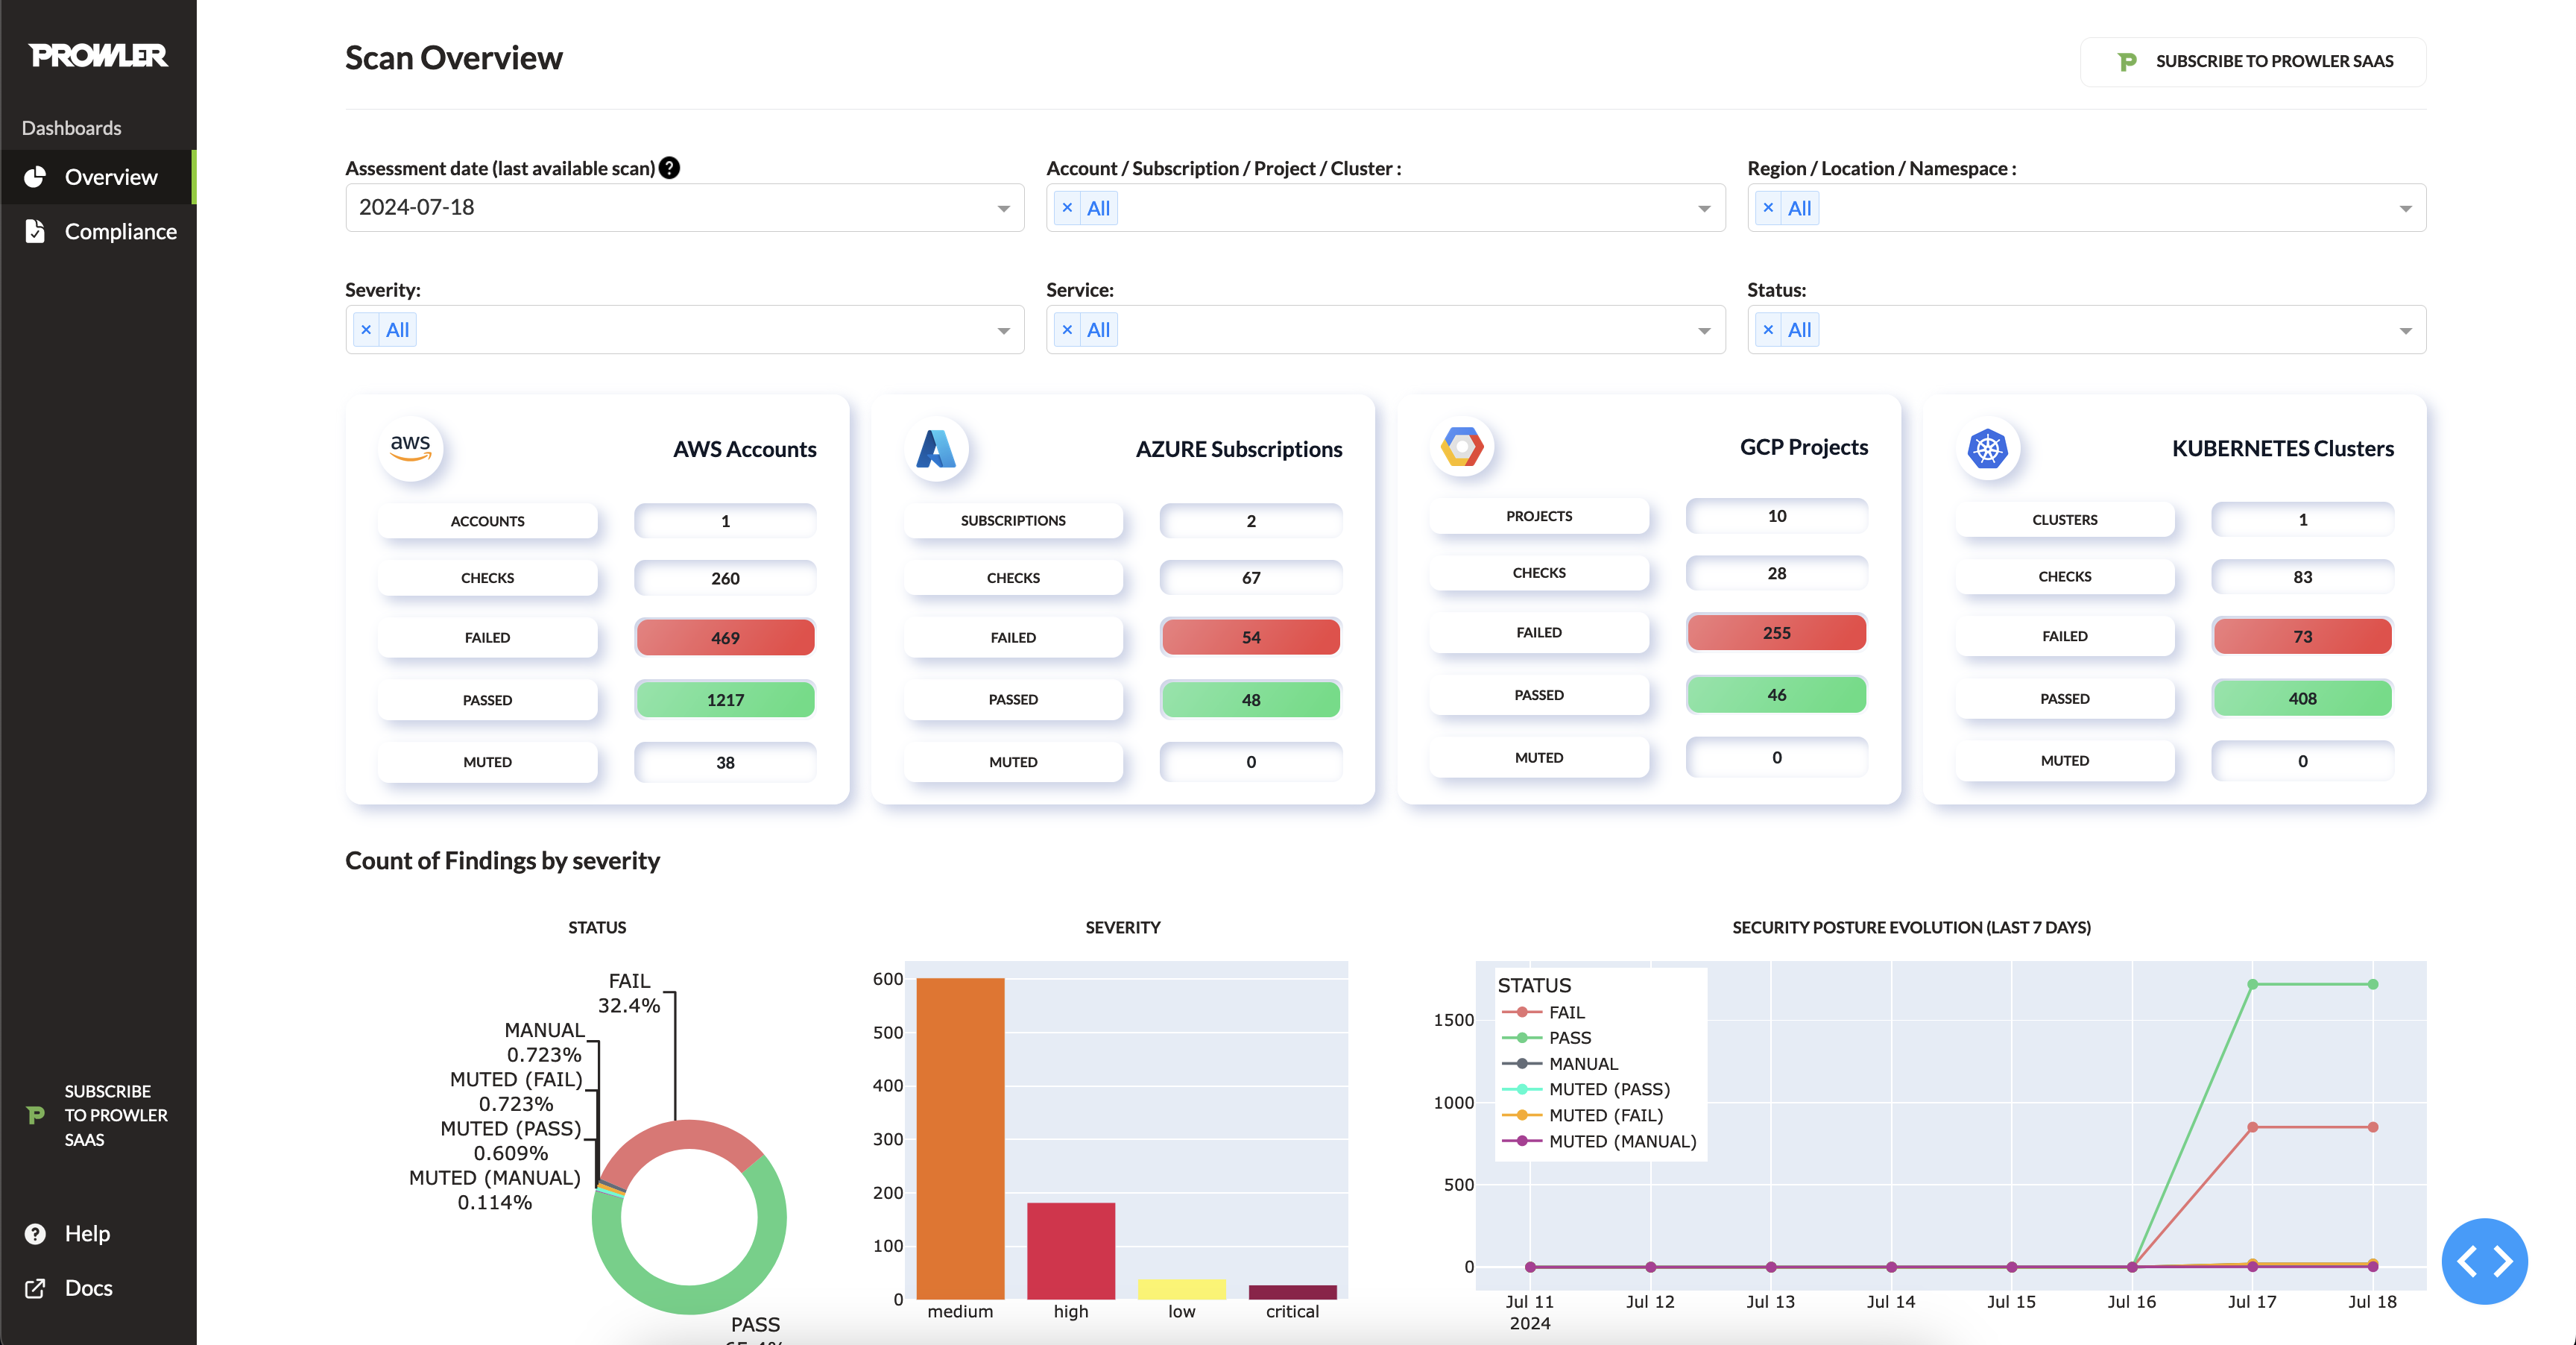
\includegraphics[width=0.85\textwidth]{images/prowler-dashboard.png}
        \caption{Prowler dashboard interface.}
		\label{img:prowler-dashboard}
	\end{center}
\end{figure}

Prowler CLI supports Azure, Google Cloud, AWS and generic Kubernetes providers. It performs a scan against multiple Kubernetes security frameworks to ensure the best coverage. Prowler supports output in CSV or JSON-OCSF format, the latter being an independent open source developed JSON schema by Open Cybersecurity Schema Framework project, which has recently joined the Linux Foundation organization. Again, we configure the Prowler job either via a configuration file or by passing the flags directly in the execution command. Listing~\ref{lst:prowler-command} provides an example on how can a Prowler scan be triggered. This particular execution would output the results in \textbf{json-ocsf} format, including only failed and manual checks.

\begin{center}
    \begin{lstlisting}[language=bash, caption={[An example of a Prowler scan command] An example of a Prowler scan command.}, label={lst:prowler-command}]
    $ prowler kubernetes \ 
        --status FAIL,MANUAL \
        --output-formats json-ocsf
    \end{lstlisting}
\end{center}

There are over a thousand issues in official Prowler Github repository. The development is still in progress and the tool receives regular updates. The project has an active community with operational development support.

\subsection{Kubescape}
Kubescape is an open-source security platform designed to harden the security of a Kubernetes cluster. Kubescape CLI allows users to scan the cluster from the local machine. Kubescape Operator enables image vulnerability scanning as well as continuous and scheduled scanning. Kubescape also offers Github Actions integration for CI/CD pipelines according to the official Github page \cite{kubescape-github}.

Kubernetes cluster is verified against a posture library (available at Github \cite{regolibrary-github}), which is a collection of frameworks each containing a set of controls. By default, the library is comprised of NSA Framework controls, MITRE ATT\&CK Framework controls and CIS Benchmark controls.

Scan configuration is again passed with multiple flags. There are flags allowing to select the namespaces to include into scan, namespaces to exclude from the scan, output format and location. Scanning can be then performed using the command displayed in Listing~\ref{lst:kubescape-command}.

\begin{lstlisting}[language=bash, caption={[An example of a Kube-bench scan command] An example of a Kube-bench scan command.}, label={lst:kubescape-command}]
    $ kubescape scan \
        --format json \
        --output kubescape-scan.json
\end{lstlisting}

Unfortunately, when executed in this mode, Kubescape performs only a few checks. In order to perform complete vulnerability and misconfiguration scan, Kubescape requires Kubescape Operator installed in the cluster. 

Kubescape's repository shows ongoing development with regular update releases.

\subsection{Preliminary Comparison}

This section compares the selected tools based on their declared feature set, ease of installation and execution, scan targets, supported cloud providers and security frameworks. This comparison does not include the analysis of the scan results, performance or any other aspects of execution. A detailed analysis of the generated reports can be found in Chapter~\ref{chap:results}.

We start by comparing the scanners by their feature set. Trivy has the most broad feature set as it is able to scan for vulnerabilities inside the images, perform IaC scan (supporting Terraform, Helm, plain Kubernetes YAML), scan for misconfigurations in Kubernetes resources and generate SBOM. Kube-bench is designed to perform only two tasks: CIS Kubernetes Benchmark checks and Node-level audit, making it very specialized tool. Prowler is able to detect misconfigurations and security threats, perform CIS Benchmark checks and cloud security audit. Kubescape's features include misconfiguration and container vulnerability scanning, RBAC risk analysis and SBOM generation. While all of the scanners can detect Kubernetes misconfigurations, only Trivy and Kubescape have the ability to scan for the vulnerabilities in containers. SBOM generation is a requirement for enterprise-level scanners nowadays, which makes Kubescape and Trivy stand out once again.

When we compare the tools by the supported cloud providers, simplicity of Kube-bench makes it the leader in this category. Since Kube-bench only performs static analysis, this makes it cloud agnostic, meaning that it can be used with any cloud provider as long as the provider offers Kubernetes services. Trivy, Kubescape and Prowler all support the same cloud providers. Kubescape and Trivy both natively support AWS, Azure and GCP. Prowler's focus is AWS, but it also supports Azure and Google Cloud Platform.

All of the presented tools declare full CIS Benchmark coverage, which is the only supported framework for Kube-bench. Trivy additionally declares NSA and MITRE ATT\&CK coverage. Kubescape further extends the set with NIST 800-53 and SOC 2 frameworks, which are more specialized frameworks, the former developed by the U.S. government and focuses on technical and administrative controls, while the latter focuses on the customer data security and compliance. Prowler mixes the CIS Benchmark checks with the four major security and privacy frameworks or regulations relevant to organizations handling sensitive data (PCI-DSS, GDPR, HIPAA, ISO27001).

From the user perspective we can compare the scanners by the ease of installation and execution. Trivy's binary is available for download using most of the popular package managers (like Brew for MacOS and apt-get, yum, pacman and others for various Linux distros). Less secure but more convenient way of installation is by using a script. Additionally, Trivy has a Docker image available in Docker Hub, GitHub Container Registry and AWS Elastic Container Registry. Trivy can be executed against an active Kubernetes context using the binary or installed as an operator inside the cluster for automatic scanning every six hours. Kube-bench can only be run from inside the container. Kube-bench provides a \textbf{job.yaml} file, which can be used to run it inside the cluster as a Kubernetes Job. Kube-bench runs checks specified in controls files that are a YAML representation of the CIS Kubernetes Benchmark checks. Kubescape supports the usual installation channels. Additionally, users are able to download scan artifacts (frameworks) separately. Kubescape Operator can be installed inside the using a Helm chart. Unfortunately, Kubescape Operator must be installed in the cluster for the Kubescape CLI to be able to scan for vulnerabilities. Prowler CLI can be installed only as a Python module, but there are also Docker images available to download from the Docker Hub and AWS Public ECR. Prowler also provides an applciation, which displays scan results in a graphical format. Table~\ref{tab:preliminary-scanner-comparison} summarizes our preliminary comparison findings.

\begin{table}[H]
    \begin{center}
        \begin{tabular}{
            | >{\raggedright\arraybackslash}p{.15\textwidth} 
            | >{\raggedright\arraybackslash}p{.22\textwidth} 
            | >{\raggedright\arraybackslash}p{.15\textwidth} 
            | >{\raggedright\arraybackslash}p{.20\textwidth} 
            | >{\raggedright\arraybackslash}p{.15\textwidth} | }
        \hline
        \textbf{Tool} & \textbf{Features} & \textbf{Cloud support} & \textbf{Frameworks} & \textbf{User experience} \\
        \hline\hline
        Trivy & Vulnerability scan, Misconfiguration scan, IaC scan, SBOM generation, Operator & AWS, Azure, GCP & CIS, NSA, MITRE ATT\&CK & CLI tool \\
        \hline
        Kube-bench & CIS Benchmark audit & cloud agnostic & CIS & Kubernetes Job \\
        \hline
        Prowler & Cloud audit, misconfiguration scan, compliance scan, Operator & AWS, Azure, GCP & CIS, PCI-DSS, GDPR, HIPAA & CLI tool, UI app \\
        \hline
        Kubescape & Operator, misconfiguration scan, vulnerability scan, SBOM generation, RBAC analysis & AWS, Azure, GCP & CIS, NSA, MITRE ATT\&CK, NIST 800-53, SOC 2 & CLI tool \\
        \hline
        \end{tabular}
    \end{center}
    \caption{Kubernetes security scanners preliminary comparison.}
    \label{tab:preliminary-scanner-comparison}
\end{table}




% \chapter{Astronomical data} \label{chap:astronomicaldata}

% nejaky obkec o tom ze data sa ziskavaju cez teleskopy a tie maju CCD chipy a ze snimky su vo formate FITS. a potom ze v tejto casti prejdeme rozne features ktore sa na snimkach nachadzaju, scenare a defekty a ako tieto nezaduce data odstranujeme
% FITS frames
% AGO data

In this section, we will first talk about how space debris images are acquired. We will describe the parameters of the telescope that captured the images used within this thesis. We will also define the format of the astronomical images. Next, we will explain what type of features can be present on the images and the defects and noises affecting them. In the last section, we present the image calibration process that is used to reduce the noises and defects to achieve clean images used for further processing and analysis. 

\section{AGO70}
The space debris images are acquired using astronomical telescopes. 
In our thesis, we are working with images captured at the Astronomical and Geophysical Observatory (AGO) in Modra. The acquisition of images at AGO is performed by the reflecting Newtonian telescope (AGO70) \cite{ago702018}, shown in the Figure \ref{img:ago70}. 

\begin{figure}[h]
    \centering
    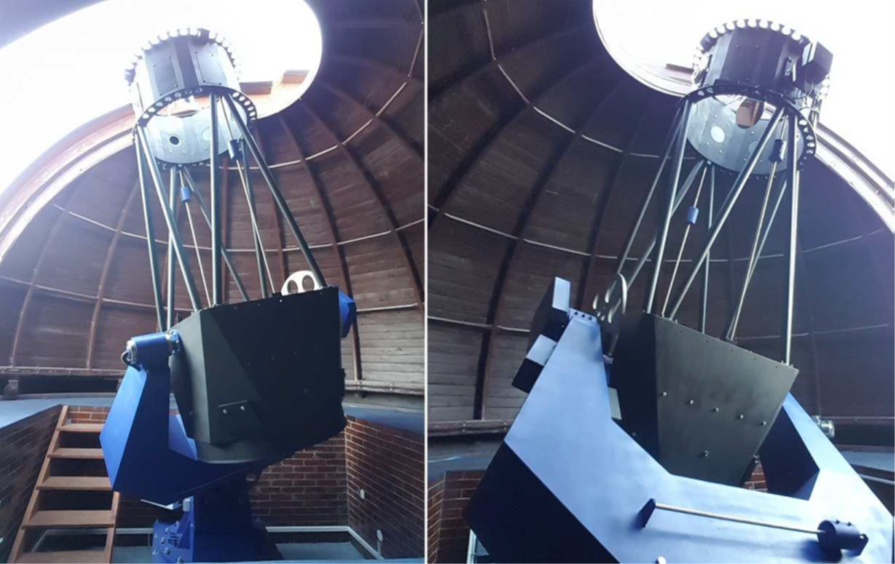
\includegraphics[width=.5\textwidth]{images/ago70.png}
    \caption{The telescope AGO70 in Modra. Source: \cite{ago702018}.}
    \label{img:ago70}
\end{figure}

In 2016, after Slovakia became the 9th member of the ESA Plan for the European Cooperating States (PECS), a contract with the Faculty of Mathematics, Physics, and Informatics (FMPI) was signed. The first action was to transform the telescope in AGO from an amateur observation tool into a professional optical system used for regular tracking of space debris. Some examples of images acquired from the space debris observations performed by AGO70 are shown in the Figure \ref{fig:ago70images}. The installation of AGO70 finished in 2016 and the telescope has the following parameters: 

\begin{itemize}
    \item 700 mm primary parabolic mirror
    \item gravity actuator supporting the parabolic mirror
    \item focal length of 2962 mm
    \item FLI Proline PL1001 Grade 1 CCD camera
    \item 24 $\mu$m pixel size of the CCD camera
    \item resolution 1024x1024
    \item 28.5' x 28.5' field of view
    \item 16 bit per pixel images
\end{itemize}


\begin{figure}[!h]
    \begin{subfigure}{.3\textwidth}
        \centering
        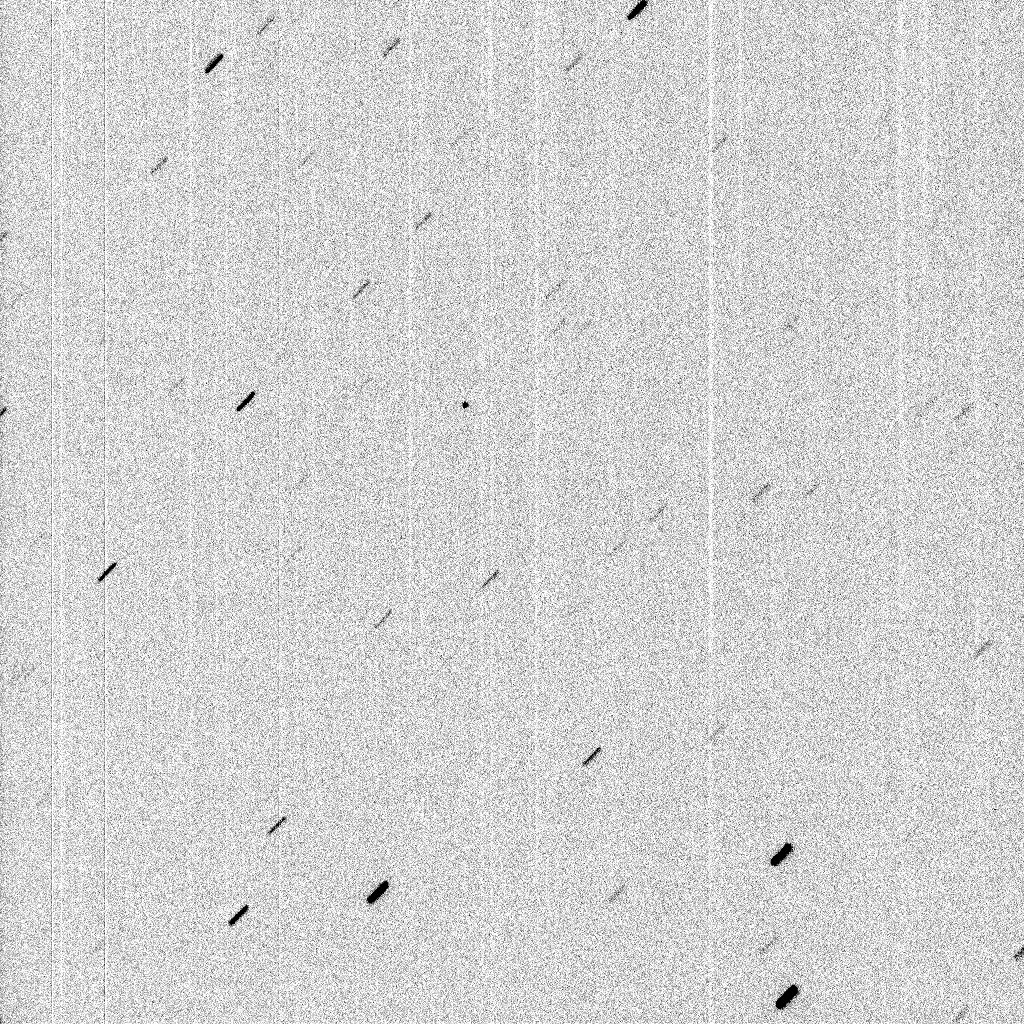
\includegraphics[width=\textwidth]{images/StreakPoint00.jpg}
    \end{subfigure}
    \hfill
    \begin{subfigure}{.3\textwidth}
        \centering
        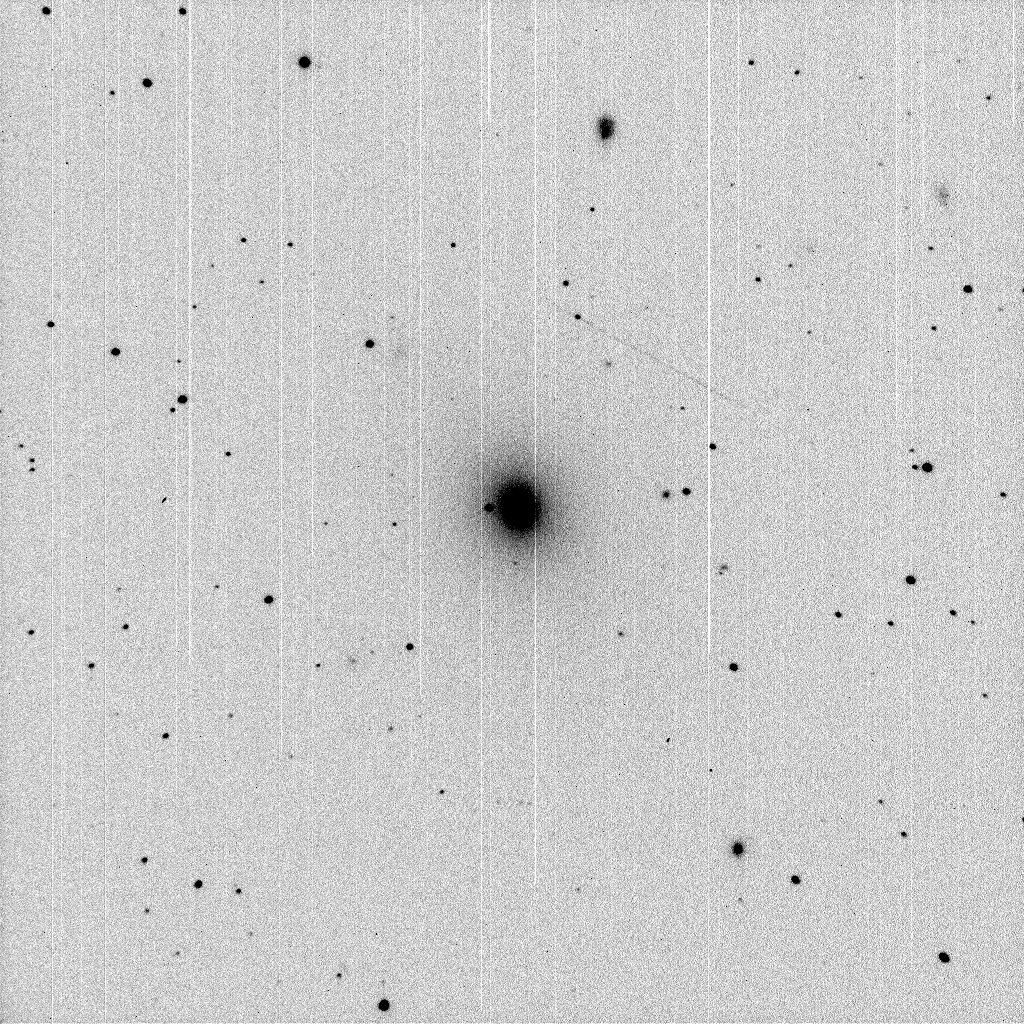
\includegraphics[width=\textwidth]{images/galaxypoints.jpg}
    \end{subfigure}
    \hfill
    \begin{subfigure}{.3\textwidth}
        \centering
        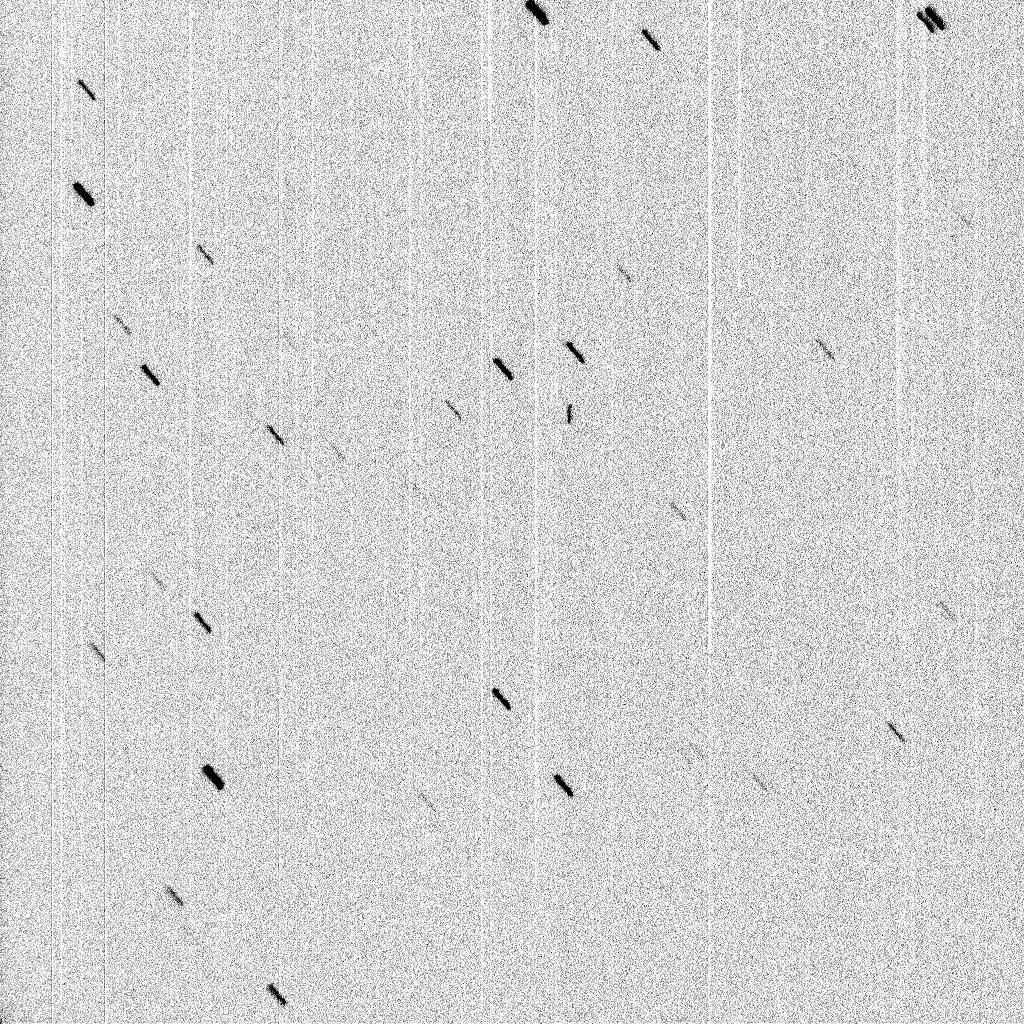
\includegraphics[width=\textwidth]{images/StreakStreak2.jpg}
    \end{subfigure}
    \hfill
    \caption{Examples of some images acquired by AGO70. }
    \label{fig:ago70images}
\end{figure}


%AGO70 has a very thin 700 mm primary parabolic mirror, which is supported by the gravity actuator. The mirror is placed at a focal length of 2962 mm. The telescope is equipped with FLI Proline PL1001 Grade 1 CCD camera and has a 28.5' x 28.5' field of view. Acquired images have a resolution of 1024x1024 pixels and contain values ranging from 0 to 65 535. 

\section{FITS format}
All images acquired from AGO70 are in the format of Flexible Image Transform System (FITS) files. It's an open standard digital format, which is very common for storing astronomical data. This data format will be used within this thesis. The structure of the FITS file is made up of two parts: header and data block \cite{fits}.

A header is a readable data structure that contains multiple keyword/value pairs. It is used for storing image metadata such as size, coordinates, and origin. With astronomical data, the header is very useful in providing photometric and spatial calibration information such as exposure time, readout noise, RADEC coordinates, etc \cite{fits}. An example of the FITS header of the image acquired by AGO70 is shown in the Figure \ref{img:fitsheader}. 

\begin{figure}[h]
    \centering
    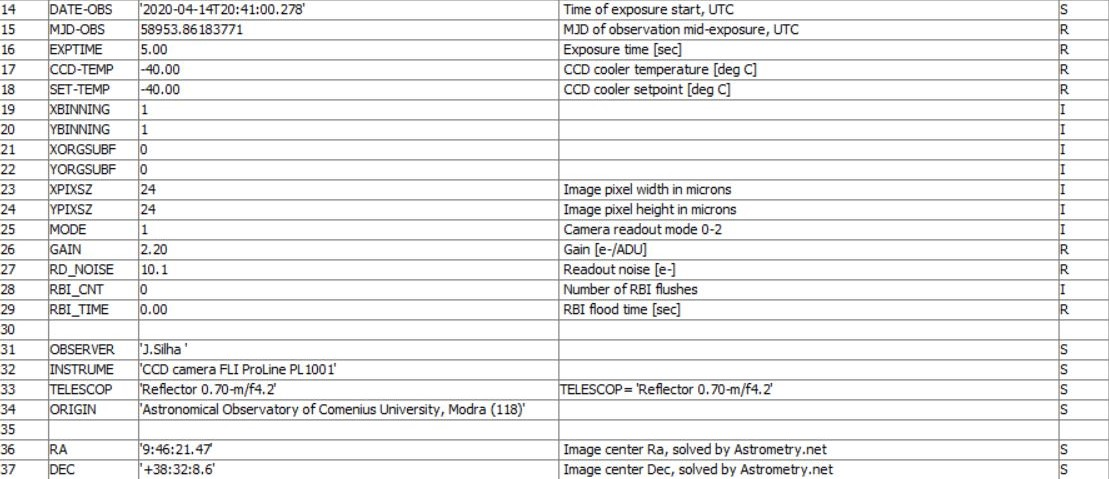
\includegraphics[width=.9\textwidth]{images/fitsheader2.JPG}
    \caption{The FITS header of the image from AGO70.}
    \label{img:fitsheader}
\end{figure}

The data block of the FITS file can store an N-dimensional array of arbitrary size. The data array usually represents an array of image pixel values or tabular data \cite{fits}.
\section{Features} \label{sec:features}
Depending on the relative position and dynamics between the observer
and the object of interest, signals from RSOs can appear differently. The most common shape is a point and streak, which will be explained in greater detail in this section. 

Moreover, other objects like galaxies, nebulas, and comets are present in the universe and can also appear in images. Their profile is significantly different from points and streaks and has more diffuse features. However, for the purpose of this thesis, we will solely focus only on galaxies and more specifically - elliptical galaxies. 
% toto neviem ci tam budem davat lebo tam chcem opisat aj galaxie
%Note, that other types of features exist. Diffuse sources like galaxies or comet tails are less common but cannot be forgotten. However, for this thesis, they are not relevant and we will solely focus only on point-like and streak-like features.   

\subsection{Point}

The shape of the point source of the light on the CCD image is defined by the point spread function - PSF. As the light is passing through the atmosphere, the point on the CCD image is smeared. The smearing effect, also called seeing, is the dominant feature of the PSF. 
Under good optic and tracking conditions, PSF is usually circularly symmetric and can be approximated using a central Gaussian core. The measure used to express the angular size of the PSF is called FWHM - full width at half maximum \cite{romanishin2006introduction}. It measures the diameter of the Gaussian core in half of its maximum amplitude as can be seen in the Figure \ref{img:fwhm0}.  

\begin{figure}[h]
    \centering
    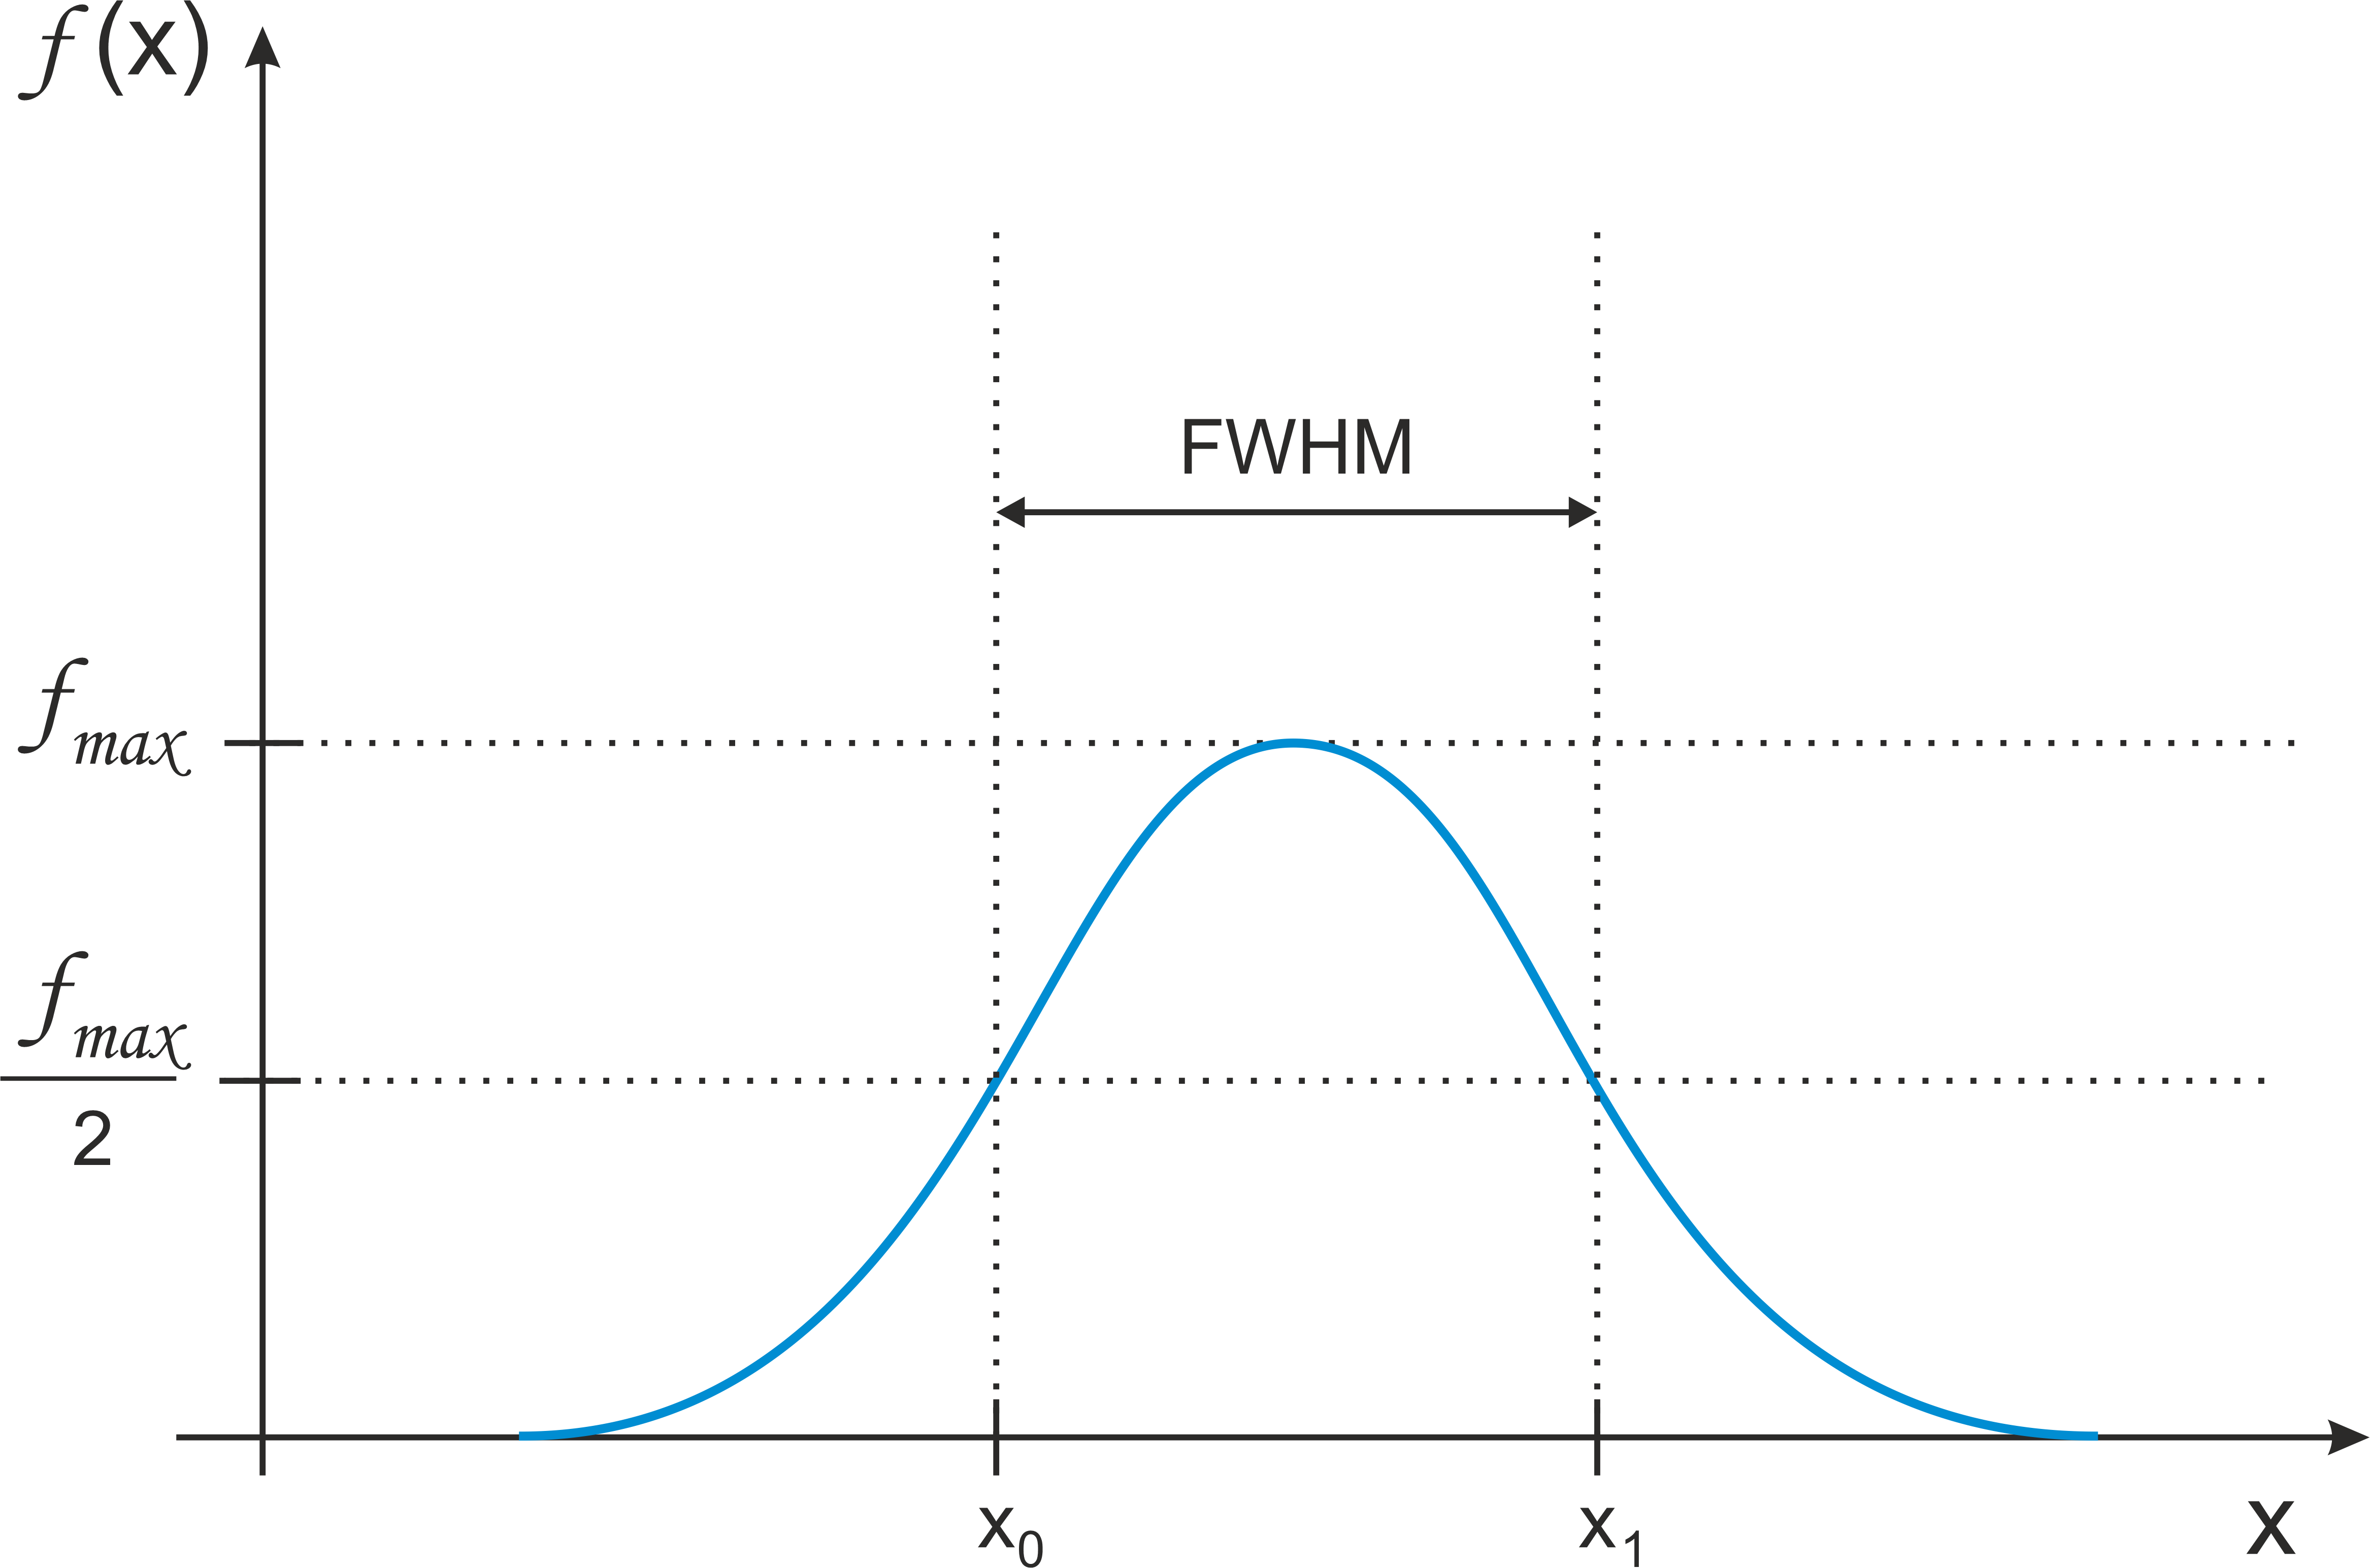
\includegraphics[width=0.5\textwidth]{images/fwhm.png}
    \caption{FWHM shown on the Gaussian curve. }
    \label{img:fwhm0}
\end{figure}

All objects that appear as points on the image, follow the PSF, and therefore all have the same FWHM and shape. However, brighter stars appear bigger on the image and this is caused by the intensity of the pixels belonging to the star \cite{romanishin2006introduction}. This phenomenon is explained in the Figure \ref{img:fwhm01}.


Another important feature of the PSF is that there is no defined edge. The intensity of the function is slowly fading until it blends with the background.


\begin{figure}[H]
    \centering
    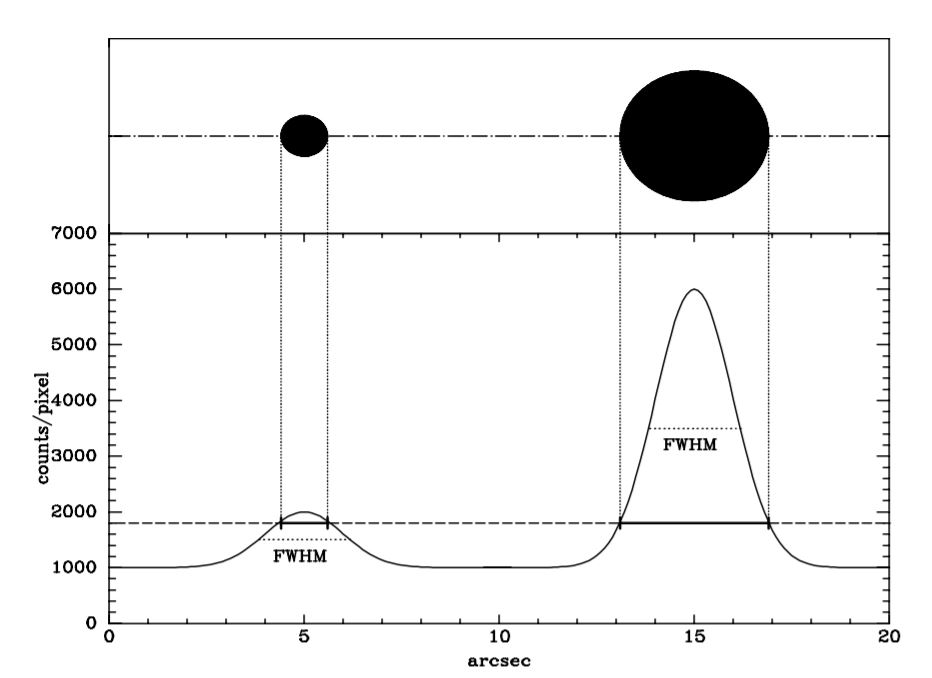
\includegraphics[width=0.7\textwidth]{images/fwhmstars.JPG}
    \caption[Comparison of faint and bright star with the same FWHM and shape]
    {
    The image shows two stars with the same FWHM, but their appearance on the frame (black dots on top of the image) differs significantly. The bright star (right) has flux five times bigger than the faint star (left). 
    On the plot in the bottom part of the image, we can observe the dashed line, which marks 1800 counts/pixel. This means that pixels below, with low intensity, are considered dark, while pixels above are considered brighter or white.  
    First, let's consider a faint star (left) which consists of a few bright pixels, but overall has a very low intensity of pixels. Low-intensity pixels appear black as they are below the dashed line. On the image, the faint star will appear smaller than the brighter star, because only the peak of the PSF will be distinguishable from the dark background. 
    Now consider a bright star (right), which has an overall very high intensity. On the image, the bright star will appear much bigger, because the majority of the PSF is above the dashed line.  
    
    Source: \cite{romanishin2006introduction}.
    
    }
    \label{img:fwhm01}
\end{figure}


\subsection{Streak}

A streak on the image, which resembles a line, can be described by its length, orientation, brightness, and width. 
Streak is approximated using multiple point-spread functions (Gaussian PSFs) moving at a constant rate in one direction and forming a line. PSFs are connected and also overlap each other to form a flat top of the streak-like shape. This function is referred to as PSF-Convolution Trail Function. % citacia

Let's situate a coordinate system on the streak. The direction in which the streak has the highest variance is the $x'$ axis and perpendicular to it is the $y'$ axis. This coordinate system is not consistent with the $(x,y)$ coordinate system of the image. This is because the streak has its orientation $\theta$ and doesn't necessarily need to be aligned with the image coordinate system. 
In this coordinate system, the length of the streak $L$ is measured on the $x'$ axis at the half-height of the function. The projection of the streak signal on the $y'$ axis creates a perpendicular profile of the streak and the width $\sigma$ of the PSF is measured at half-width. This is illustrated in the Figure \ref{img:line0}. 
The flux $f$ of the streak at any point situated in the new orthogonal coordinate system $(x',y')$ can be expressed as:

\begin{equation}
    f(x',y') = b(x',y') + \frac{\Phi}{L} \cdot \frac{1}{\sqrt{2 \pi \sigma^2}} \cdot \int_{-L/2}^{+L/2} 
    exp \left(  
        - \frac{1}{2 \sigma^2} \cdot \left[ (x' - l)^2 + (y')^2 \right]
    \right) \,dl
\end{equation}

where $\Phi$ is the total photometric flux in the streak and $b(x',y')$ is the background flux at the same point \cite{thesisNagy}. 


\begin{figure}[h]
    \centering
    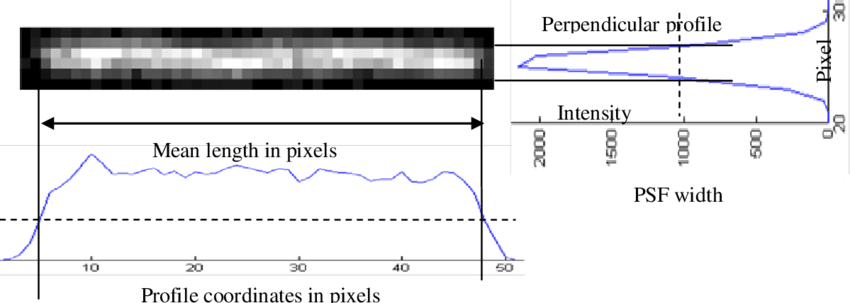
\includegraphics[width=0.7\textwidth]{images/line.png}
    \caption[Length and width of the streak on the image]
    {Length and width of the streak explained on the image.
    Image source: \cite{articleStreaks}.}
    \label{img:line0}
\end{figure}

\subsection{Galaxy}
According to \cite{hubble} galaxies can be classified into 3 categories based on their visual appearance:
\begin{itemize}
    \item Elliptical 
    \item Spiral 
    \item Lenticular
\end{itemize}

In this thesis, we will only focus on the elliptical galaxies, which in the case of modeling and using ellipticity of 1 can also be a good approximation of spiral and lenticular galaxy shapes to be used for the training purposes.

The main characteristic of an elliptical galaxy is that its profile resembles ellipses on the images. They are highly concentrated and the light going from the center fades smoothly and rapidly away. This creates a smooth diffuse profile with an undefined edge. Another interesting feature of elliptical galaxies is that with increasing exposure time of the image, the diameter of the galaxy is steadily increasing but the shape stays roughly the same \cite{hubble}.

Elliptical galaxies are denoted with the letter "E". In full notation "E" is followed by a number representing their degree of ellipticity, which is defined as follows: 

\begin{equation}
E = \frac{(a-b)}{a}
\end{equation}

where $a$ is the major diameter and $b$ is the minor \cite{hubble}. 

\section{Scenarios} \label{sec:scenarios}

In this section, we will explain different scenarios happening during the image capture, that affect how the object appears in the image. Scenarios depend on the mode of tracking (sidereal, object) and the relative velocity between the moving object of interest and the telescope. 

\subsection{Point-like stars, point-like objects}
This is a typical scenario occurring in astronomical images and is shown in the Figure \ref{fig:pointpoint1}. The angular velocity of the moving object of interest is so small that during the exposure time their position on the image doesn't seem to move. The speed is so slow that they don't cross more than one pixel, which leads to the appearance of the object as a point. This applies to both, objects of interest as well as stars. 

This scenario commonly happens in an asteroid field, small solar body system field, and can also appear in space-debris observations when high cadence and low exposure time is used. 

\begin{figure}[!h]
    \centering
    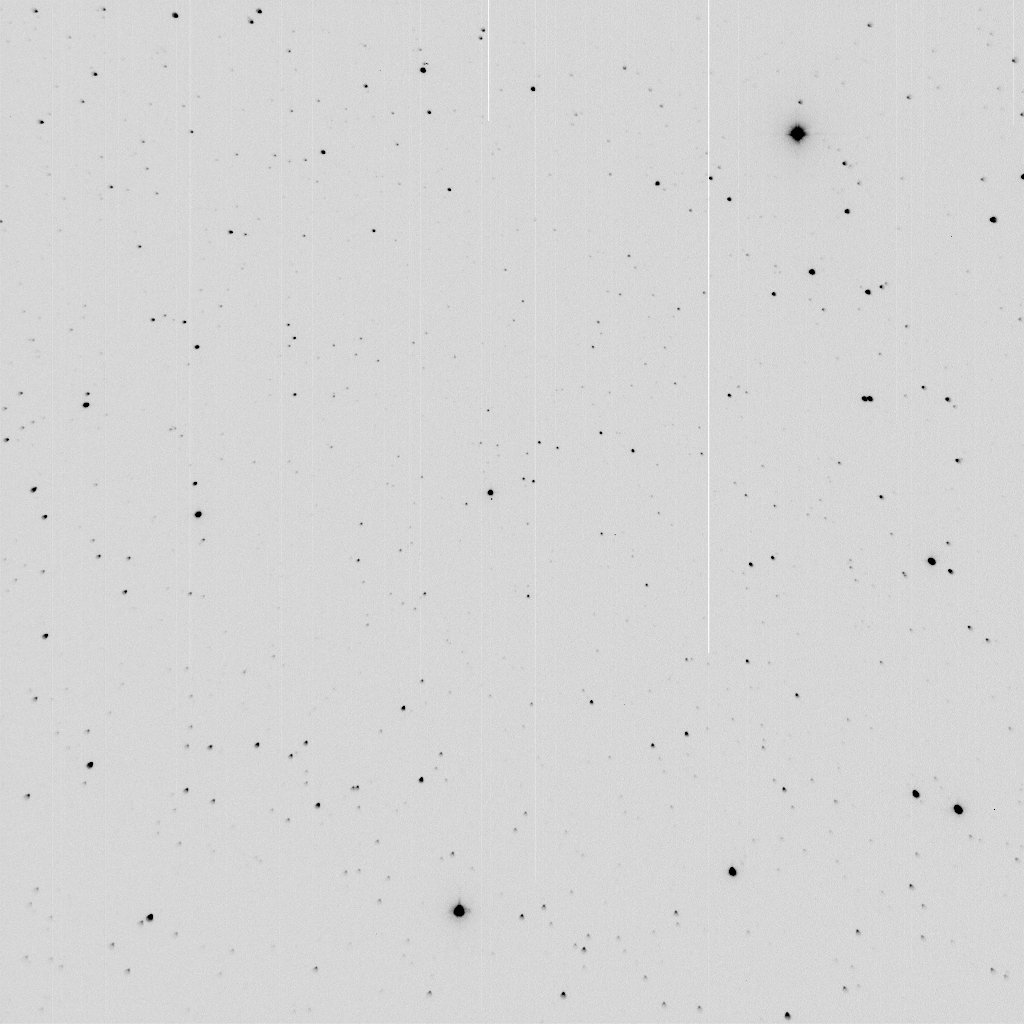
\includegraphics[width=.4\textwidth]{images/PointPoint.png}
    \caption{An example of point-point scenario.}
    \label{fig:pointpoint1}
\end{figure}

\subsection{Point-like stars, streak-like objects}
In ground-based images, stars appear as points, due to slow relative dynamics between the observer. If the exposure time on the image was longer stars would appear as streaks too, as a result of the motion of the Earth. 
During sidereal tracking, the telescope is moving to compensate for the Earth's motion and this results in point-like stars remaining in the same place on images.
In space-based images, stars appear as points if the camera is fixed.


Regarding moving objects, if the exposure time is long enough that the object is crossing more than one pixel, they appear as streaks. This commonly happens when the object is moving with high velocity. %If the exposure time is long compared to the angular velocity, it leads to objects appearing as streaks. 

The point-like stars and streak-like object scenario can be observed in the series of images depicted in the Figure \ref{fig:pointstreak0}.

%However if the exposure time is too short for an object to cross more than one pixel it would appear as a point, which is the point-point scenario explained above. 

\begin{figure}[!h]
    \begin{subfigure}{.3\textwidth}
        \centering
        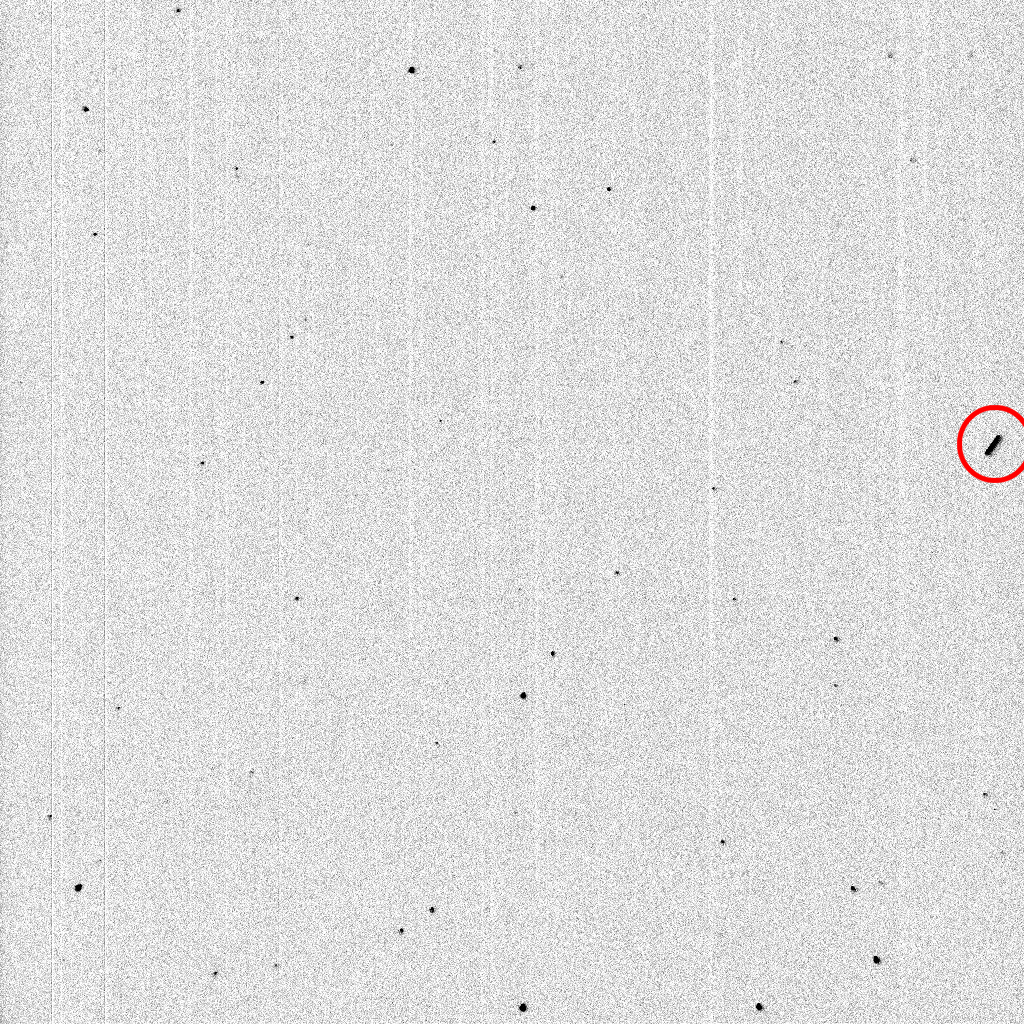
\includegraphics[width=\textwidth]{images/PointStreak1.png}
        \label{fig:pointstreak1}
    \end{subfigure}
    \hfill
    \begin{subfigure}{.3\textwidth}
        \centering
        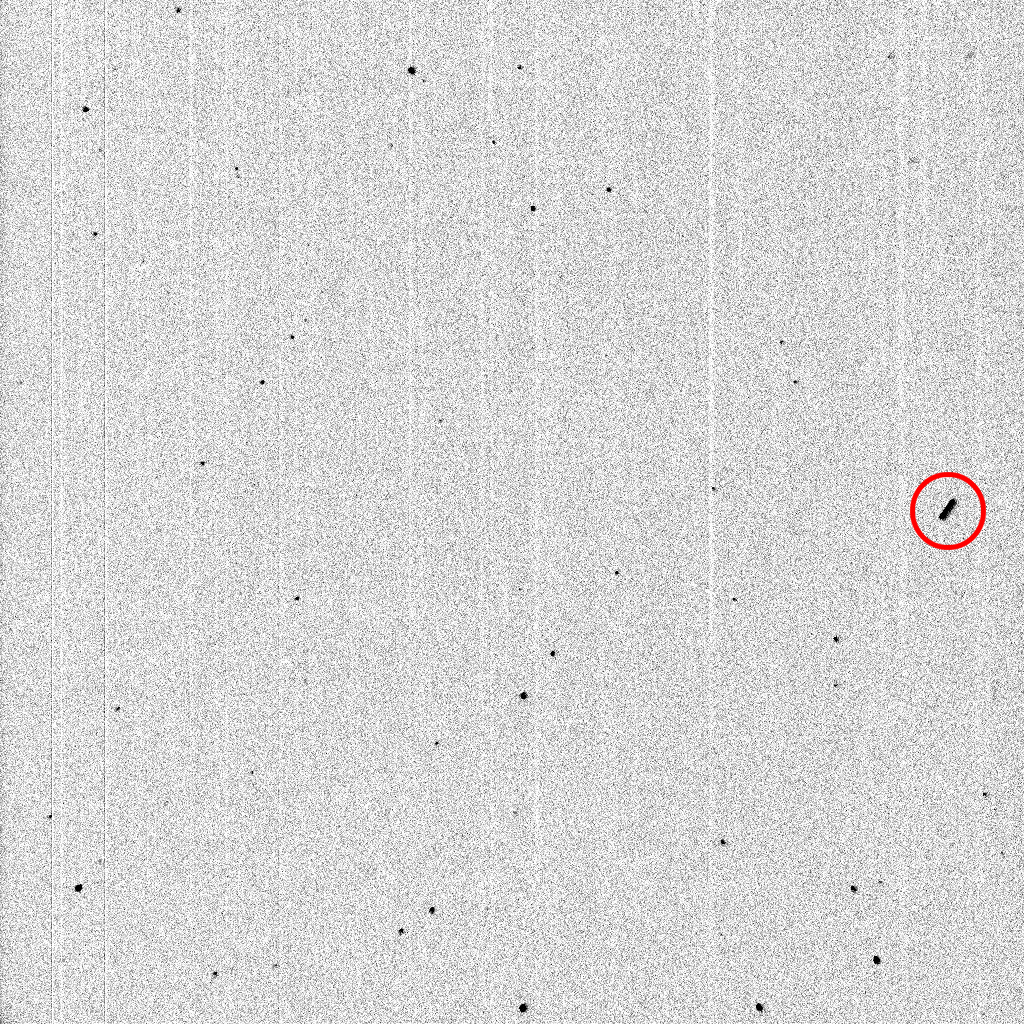
\includegraphics[width=\textwidth]{images/PointStreak2.png}
        \label{fig:pointstreak2}
    \end{subfigure}
    \hfill
    \begin{subfigure}{.3\textwidth}
        \centering
        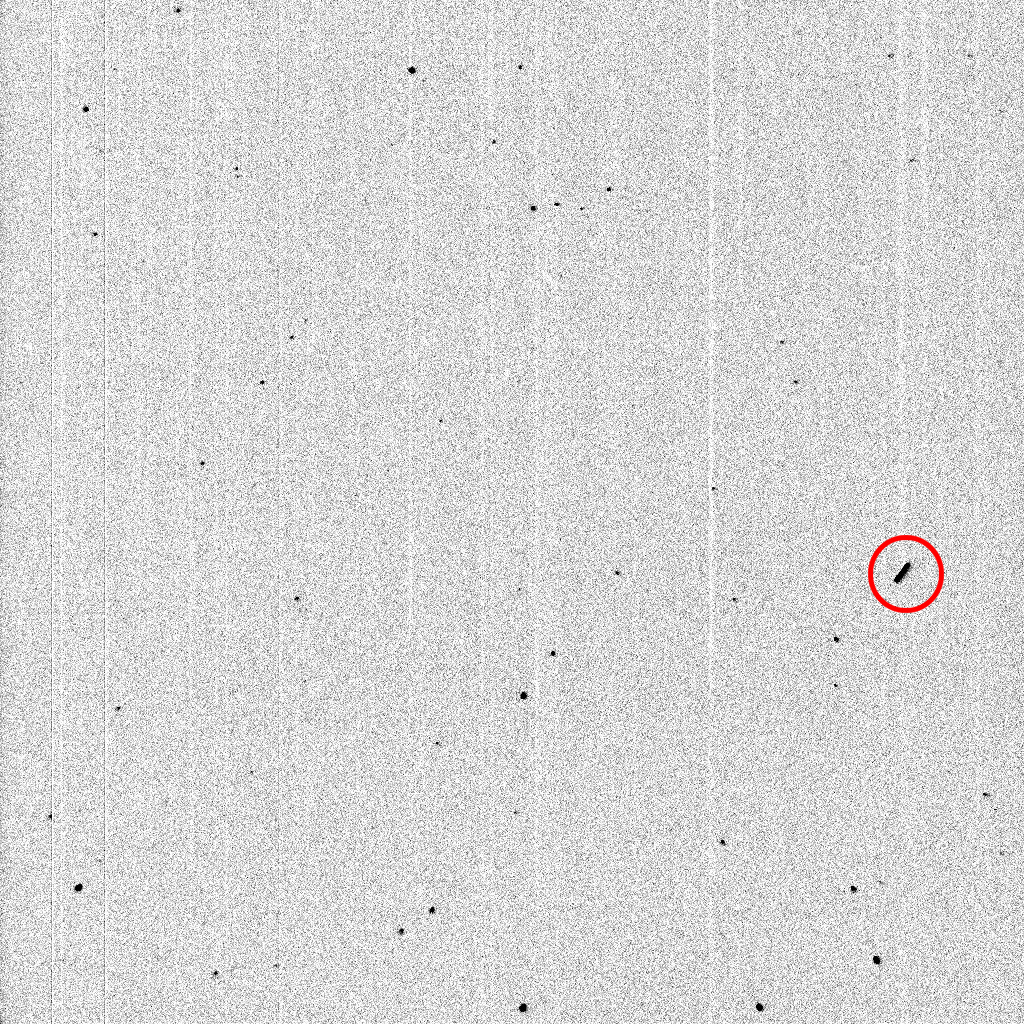
\includegraphics[width=\textwidth]{images/PointStreak3.png}
        \label{fig:pointstreak3}
    \end{subfigure}
    \hfill
    \caption{An example of series of images capturing a streak-like object and point-like stars. }
    \label{fig:pointstreak0}
\end{figure}

\subsection{Streak-like stars, point-like objects}
When the telescope is in object tracking mode, the focus is aimed at the moving object. Thus telescope is following the object matching its speed and direction. The moving object, therefore, appears as a point while stars appear as streaks. All stars will have the same length and direction of the streak-like shape. An example of one point-like object and otherwise streak-like stars are shown in the Figure \ref{fig:streakpoint0}. 

If there are more moving objects present on the frame, they can either appear as points or streaks. In case the other moving objects are moving at a similar speed and direction as the tracked object, they will also appear as points. This scenario happens when a telescope is tracking a cluster of objects. Otherwise, if other objects have different speeds and directions, they will appear as streaks but with different lengths and directions as streaks created by stars. 
This applies to both, space- and ground-based images. All these effects can influence the performance of segmentation or recognition algorithms.

\begin{figure}[!h]
    \begin{subfigure}{.3\textwidth}
        \centering
        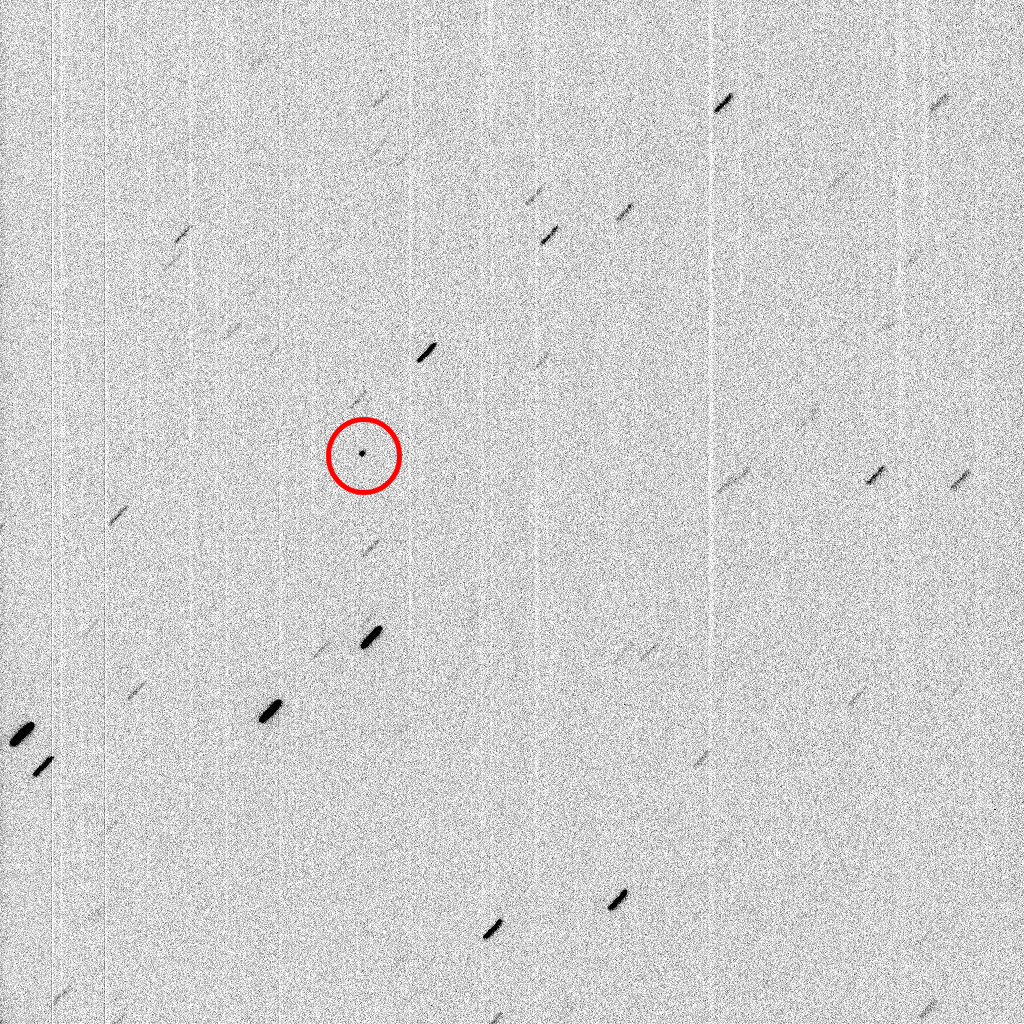
\includegraphics[width=\textwidth]{images/StreakPoint1.png}
        \label{fig:streakpoint1}
    \end{subfigure}
    \hfill
    \begin{subfigure}{.3\textwidth}
        \centering
        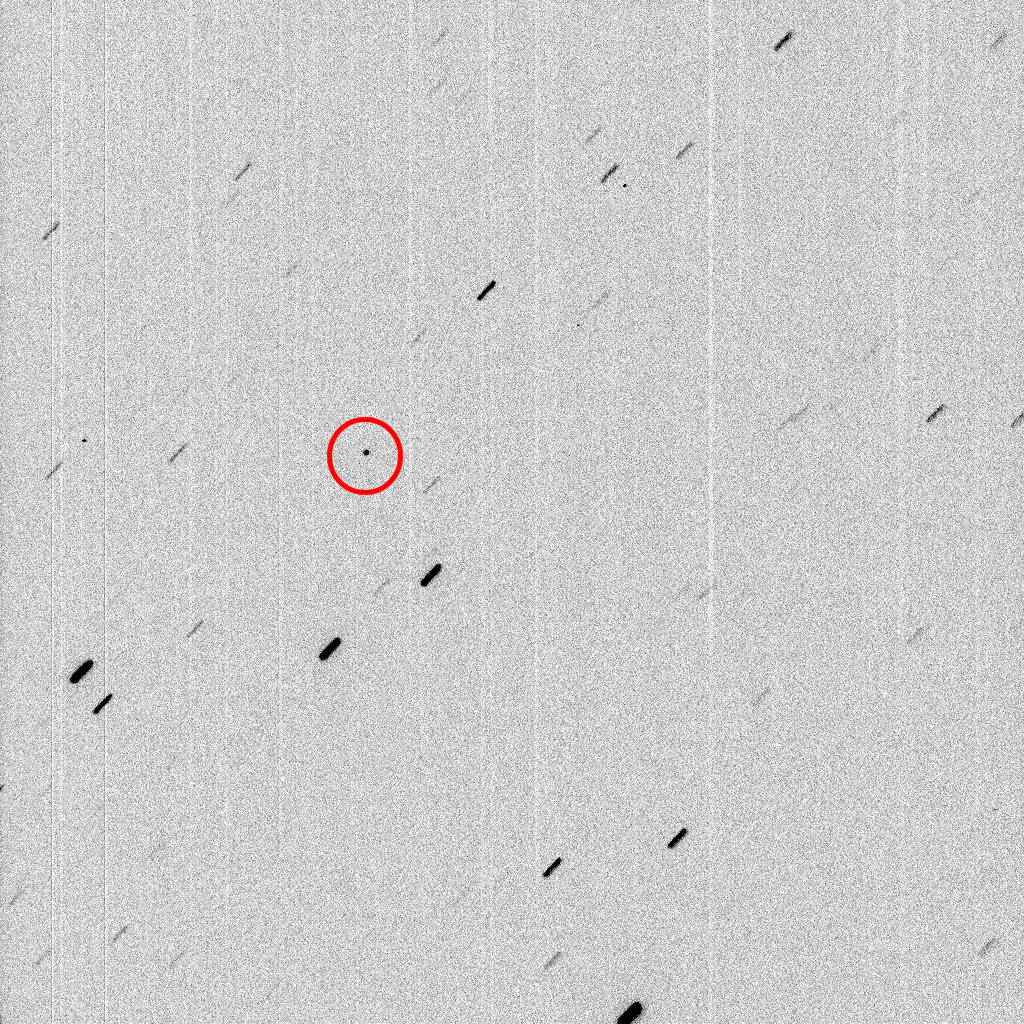
\includegraphics[width=\textwidth]{images/StreakPoint2.png}
        \label{fig:streakpoint2}
    \end{subfigure}
    \hfill
    \begin{subfigure}{.3\textwidth}
        \centering
        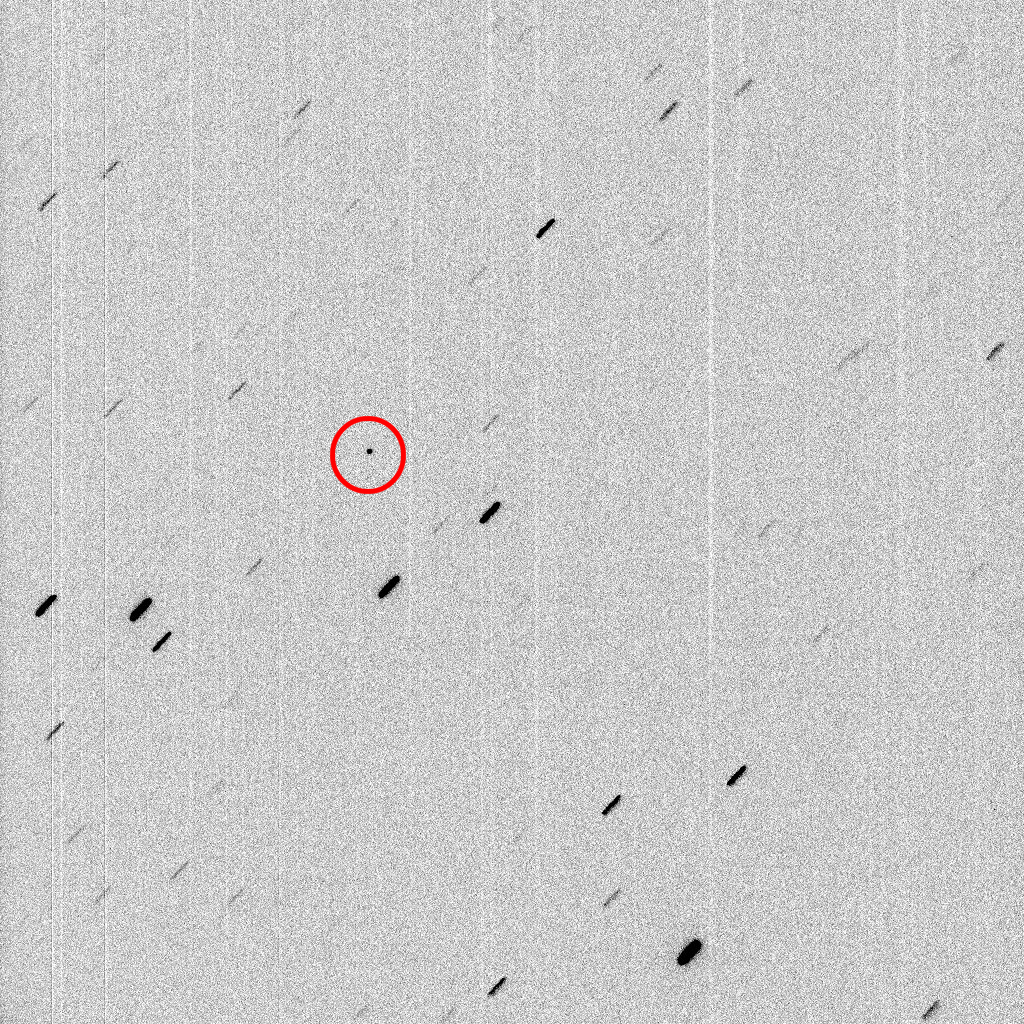
\includegraphics[width=\textwidth]{images/StreakPoint3.png}
        \label{fig:streakpoint3}
    \end{subfigure}
    \hfill
    \caption{An example of series of images capturing a streak-like stars and one point-like object. }
    \label{fig:streakpoint0}
\end{figure}

\subsection{Streak-like stars, streak-like objects}
This is a common scenario happening during the survey of the sky, when stars nor objects are being tracked, which is depicted in the Figure \ref{fig:streakstreak0}. When taking an image of the sky field during the survey, unknown objects can appear randomly, leaving streak-like features of different lengths and directions on the image. 
Stars appear as streaks in ground-based observations due to the motion of Earth and long exposure time. However streak-like stars can also be caused by the motion of the telescope in both ground and space-based observations. 

\begin{figure}[!h]
    \begin{subfigure}{.3\textwidth}
        \centering
        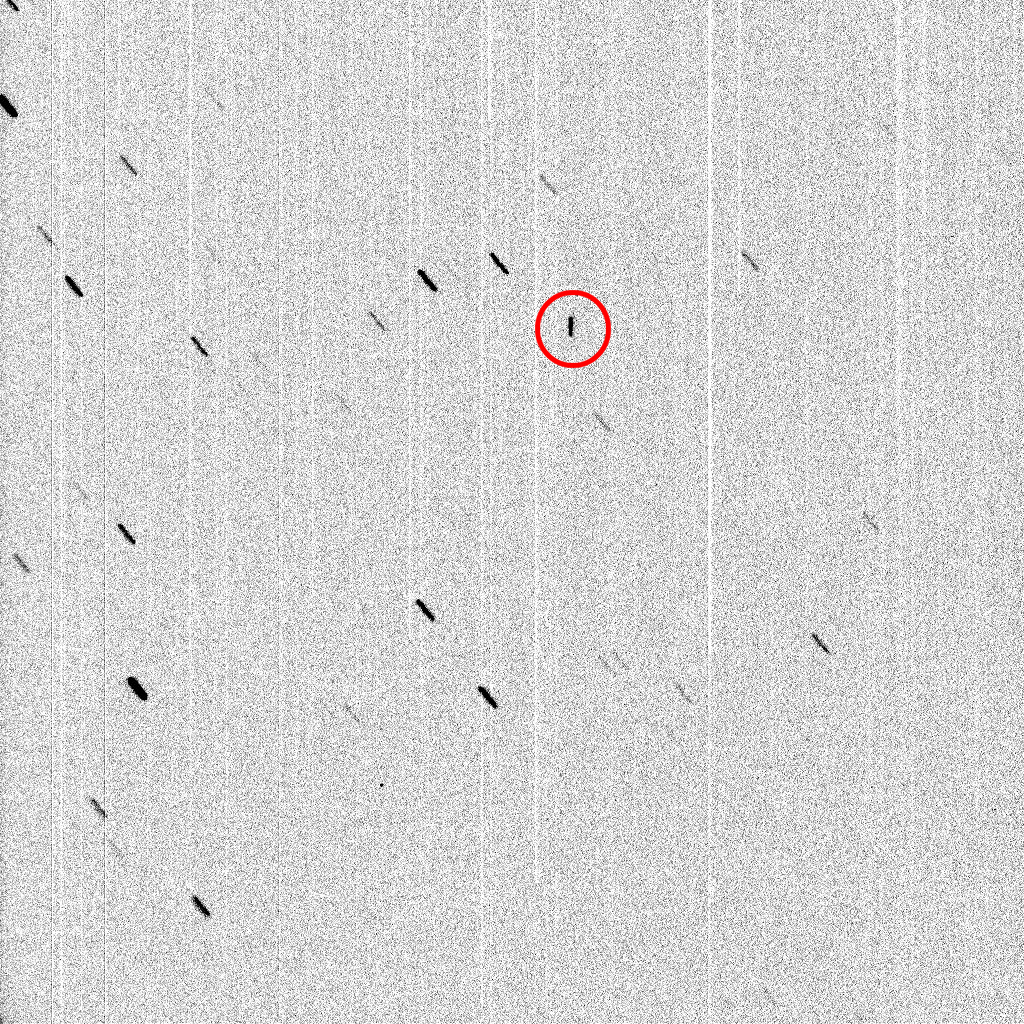
\includegraphics[width=\textwidth]{images/StreakStreak1.png}
        \label{fig:streakstreak1}
    \end{subfigure}
    \hfill
    \begin{subfigure}{.3\textwidth}
        \centering
        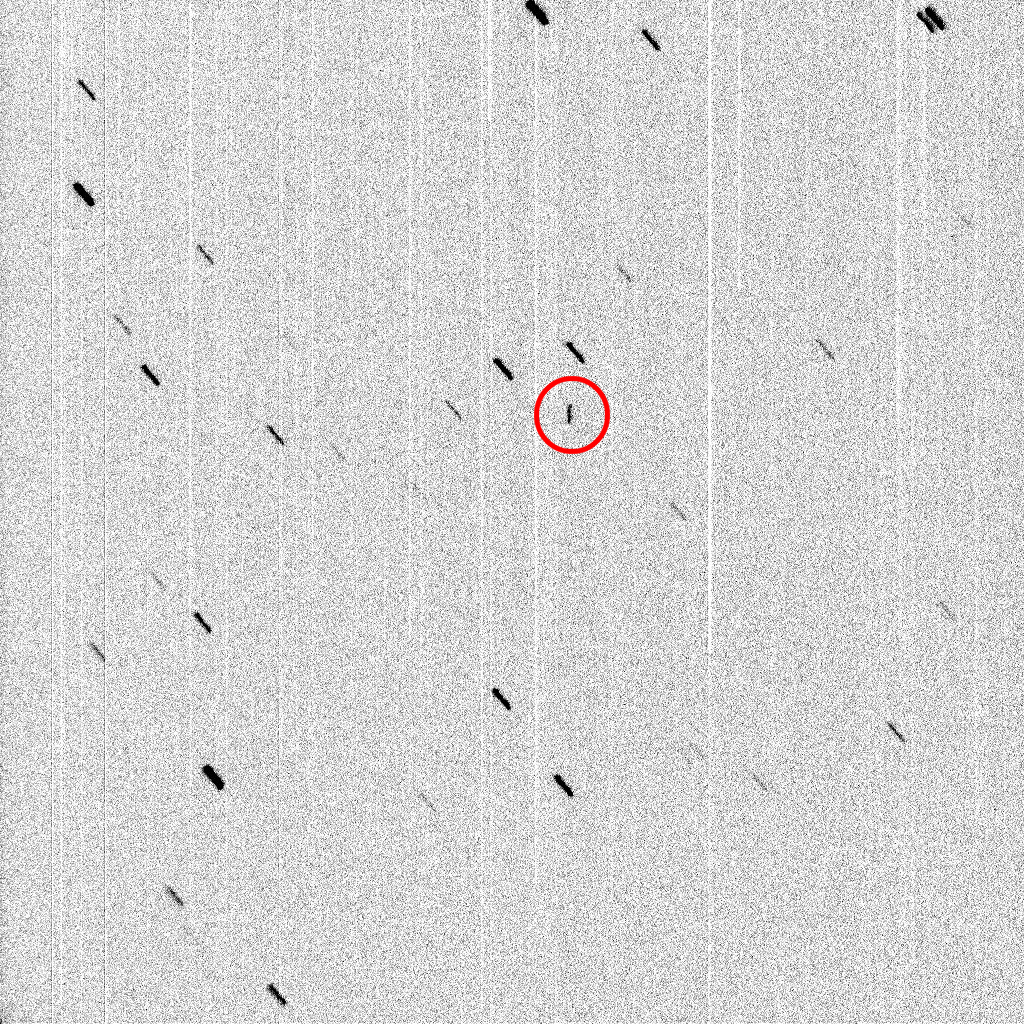
\includegraphics[width=\textwidth]{images/StreakStreak2.png}
        \label{fig:streakstreak2}
    \end{subfigure}
    \hfill
    \begin{subfigure}{.3\textwidth}
        \centering
        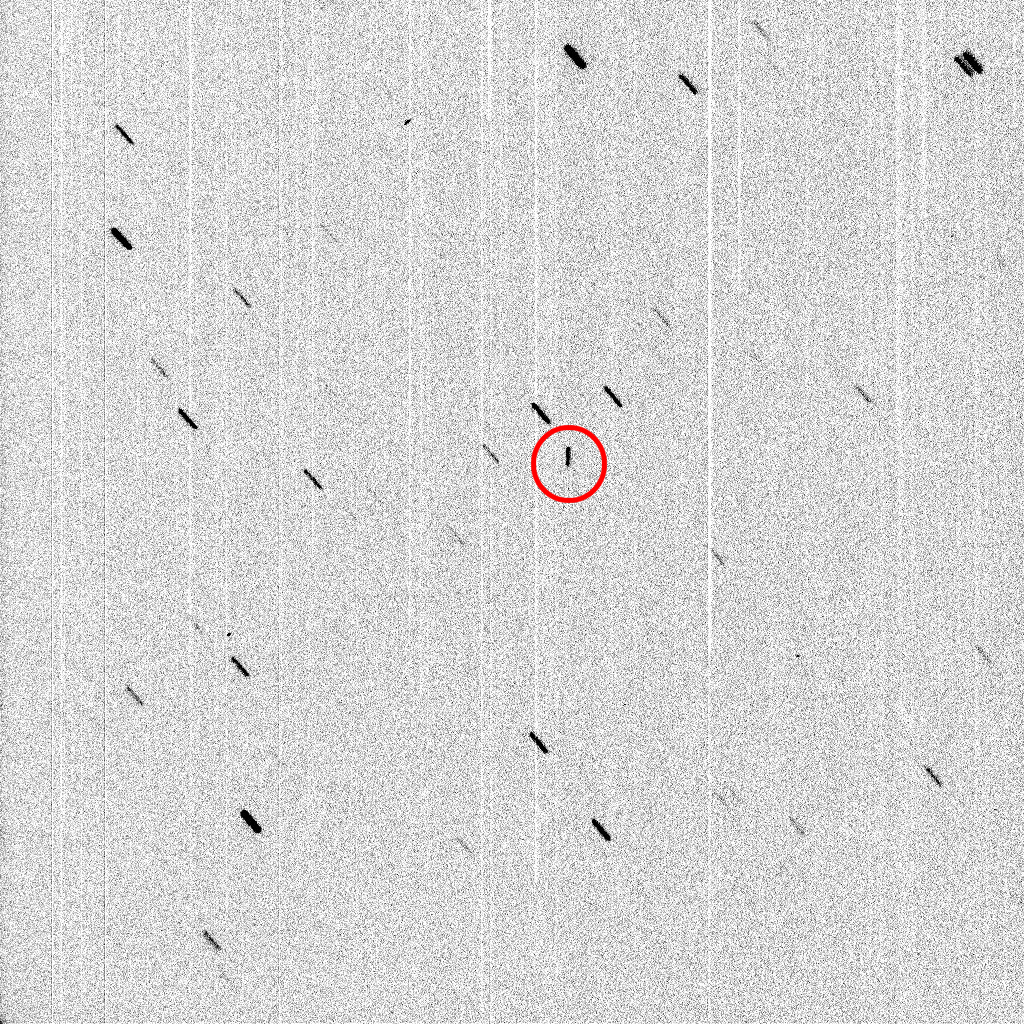
\includegraphics[width=\textwidth]{images/StreakStreak3.png}
        \label{fig:streakstreak3}
    \end{subfigure}
    \hfill
    \caption{An example of series of images capturing a streak-like stars and one streak-like object. }
    \label{fig:streakstreak0}
\end{figure}

\subsection{Supported defects and noises}
To make images realistic, defects and noises that corrupt real astronomical images were added to the generator. 
This includes noises such as Gaussian noise and Poisson noise and defects like hot pixels and cosmic rays. We are aware that some noises and defects are missing. However, the data generator was not the primary focus of the thesis and was only a secondary tool to generate images for training purposes. Yet to make up for missing noises, we added the option to use real BIAS, DARK and FLAT FIELD frames in the generation. These real frames already include readout noise, bias voltage, dark current, dead columns, dust rings, vignette, and others (more info in Section \ref{sec:defects}). 

\subsubsection{Gaussian noise}
Gaussian noise is used to simulate the sky background noise. It is applied to each frame separately to keep the randomness in the images. The user can define the $mean$ and standard deviation ($std$) of the noise.

\subsubsection{Poisson noise}
Poisson noise is applied to each generated object to simulate the photons falling onto the chip. In the configuration file, the user can define if he wants to apply the Poisson noise using the $applyPoisson$ boolean parameter. 

\subsubsection{Hot pixels}
In the generation of hot pixels on the image, the user can set their $count$ and $brightness$. In generated series, hot pixels are static and stay at the same position in all frames. 

\subsubsection{Cosmic rays}
In the configuration file, the user can set the number of generated cosmic rays with $count$, as well as their $brightness$. In Section \ref{sec:defects} we mentioned three different types of cosmic rays: spots, tracks, and worms. Spots usually have fewer pixels than tracks and worms, which is why the user can define the number of pixels using $spotPixelCount$ for spots and $pixelCount$ for tracks and worms. Cosmic rays are generated randomly for each frame since in the real observations they occur randomly as well.

\subsubsection{BIAS, DARK, FLAT FIELD frames}
When using real frames, the user must define the path to the real images using parameter $dataDir$. Important to note, that the images must have the same dimensions as the generated image, or else it will not work correctly. The same real frames are applied to each frame after all objects are generated. First, we multiply the image with the values from the FLAT FIELD frame, which defines the pixel sensitivity. DARK and BIAS frames are added afterward. DARK frames usually already contain bias voltage, so we don't need to apply the BIAS frame.




\section{Photometric reduction of CCD images} \label{sec:photoreduction}


An image obtained by a telescope using a CCD camera is called a raw image. A raw image is affected by before mentioned defects and noises. Therefore, the image needs to be corrected to a certain level to obtain precise photometric results \cite{articleParimucha}. This process is called image calibration, which contains several steps discussed here below.  

\subsection{Calibration images}
The image calibration consists of three steps: subtraction of BIAS image, subtraction of DARK image and division by FLAT FIELD image.

    %%%%%%%%%%%%%%%%%%%%%%%%%%%% 
    \subsubsection{BIAS frame}
    As mentioned earlier, to solve an issue with negative values in ADC, bias voltage was introduced.
    However, during photometry, the offset bias value needs to be subtracted from the image to achieve correct values. To retrieve the bias values on the pixels, the BIAS frame is created. 
    The aim is to retrieve an image without any residual signal in the pixels originating from the camera. This is achieved by taking an image with a closed shutter and zero exposure time \cite{articleParimucha}.
     
             
    %%%%%%%%%%%%%%%%%%%%%%%%%%%%   
    \subsubsection{DARK frame} 

    DARK frames are introduced to detect dark current in the image. Apart from that, they are also capable of detecting hot and dead pixels on the image. 
    To create a DARK frame, an image is taken with a closed shutter to eliminate photo-electrons from stars and the sky. Values in the pixels are from the dark current and bias voltage. Therefore to obtain a correct DARK frame, bias values need to be subtracted from the DARK frame. 
    As mentioned before, dark current is proportional to chip temperature and exposure time. This implies that in order to have correct dark current values, the DARK frame needs to be taken with the same exposure time as the raw image. The same goes for the temperature of the CCD chip \cite{articleParimucha} \cite{articleCcdOnline} \cite{phy217}. 
    

    %%%%%%%%%%%%%%%%%%%%%%%%%%%%  
    \subsubsection{FLAT FIELD frame} 
    
    Taking an image of the perfectly uniform light source, would not result in an image with the same amount of counts in each pixel. Readout noise, bias voltage, and dark current are all contributing to this fact. However, even without them, the image would not be uniform. The main reason is the sensitivity of each pixel. Due to the manufacturing limitations, no two pixels convert the light photons into electrons the same way \cite{articleCCDartifacts} \cite{phy217}.
    
    The solution to this problem is by taking a FLAT FIELD frame, which corrects pixel to pixel sensitivity. As mentioned before, the frame is created by taking a picture of an evenly illuminated field. One of the most common ways is to take an image of the twilight sky.
    Similarly, as with the DARK frame, this FLAT FIELD frame contains values from bias voltage as well as dark current. To get a single correct FLAT FIELD frame, these values need to be subtracted.
    Another great feature of the FLAT FIELD frame is that it can also detect dust particles on the filters and lenses. These manifest as dark rings on the image. They are the same with different exposure times but vary from filter to filter. However, they also differ from time to time as some particles can be shifted, eliminated, or added. 
    Furthermore, flat fielding can clear dimming on the edge of the image. This is also called vignetting and is caused by out-of-focus obstructions in the light path \cite{articleParimucha} \cite{phy217}.
    
    After taking the FLAT FIELD frame, signal values are arbitrary, since it only means how bright the source of illumination was. The important part is the differences in the signal across the chip. FLAT FIELD frame is therefore normalized in a way that the average signal in each pixel is 1 \cite{phy217}.
    %% najst citaciu tohto
    
        
    %%%%%%%%%%%%%%%%%%%%%%%%%%%%  
    \subsubsection{MASTER frame}
    
    Due to the nature of reading the image from the CCD chip, every calibration image contains readout noise, which can cause issues during the calibration process. To minimize the noise, multiple calibration images are taken, which are then reduced to one MASTER frame. 
    The MASTER frame is created by taking average or median values of the pixel from the multiple calibration images (BIAS, DARK, FLAT FIELD).
    After the process, we have MASTER BIAS, MASTER DARK, and MASTER FLAT FIELD frames (shown in the Figure \ref{fig:masterframes}), and these are later used in photometric reduction \cite{articleParimucha}.
   
   
   
    \begin{figure}[!h]
    \centering
        \begin{subfigure}[t]{.3\textwidth}
            \centering
            
\includegraphics[width=\textwidth]{images/biasframe.jpg}
            \caption{MASTER BIAS frame.}
            \label{fig:biasframe}
        \end{subfigure}
        \hfill
        \begin{subfigure}[t]{.3\textwidth}
            \centering
            
\includegraphics[width=\textwidth]{images/dark90s.jpg}
            \caption{MASTER DARK frame with exposition time of 90 seconds.}
            \label{fig:darkframe}
        \end{subfigure}
        \hfill
        \begin{subfigure}[t]{.3\textwidth}
            \centering
            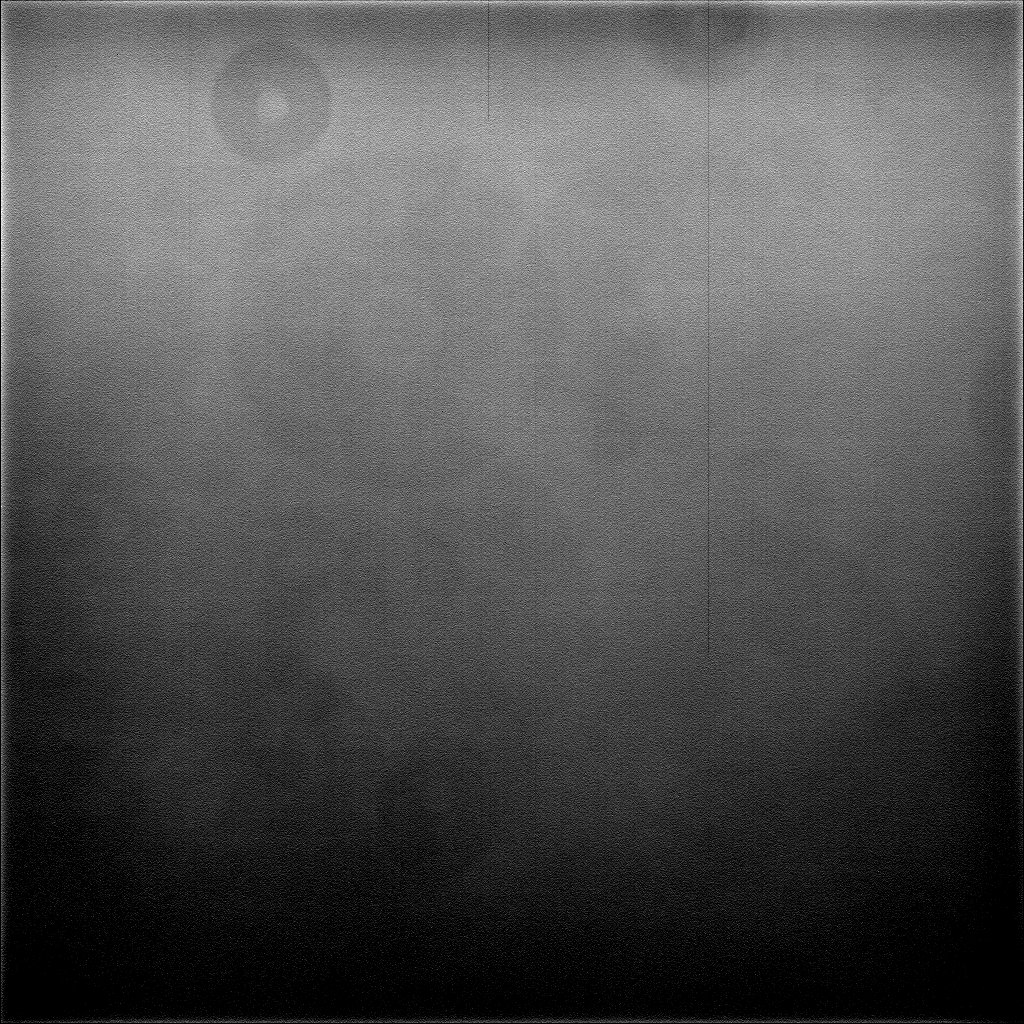
\includegraphics[width=\textwidth]{images/flatframe.jpg}
            \caption{MASTER FLAT FIELD frame.}
            \label{fig:flatframe}
        \end{subfigure}
        \hfill
        \caption{Examples of MASTER frames acquired by AGO in Modra.}
        \label{fig:masterframes}
    \end{figure}



\subsection{Formal definition}

The intensity of the raw image at the pixel $(x,y)$, with exposure time $t$ and temperature of CCD chip $T$ can be generally written as
\[ I(x,y,t,T) = b(x,y,T) + d(x,y,t,T) + i(x,y,t,T) f(x,y,t_f,T) \]

where $b(x,y,T)$ is the intensity of BIAS frame. Exposure time is ommited since the BIAS frame is taken with exposure time of zero. Intensity of DARK frame is denoted as $d(x,y,t,T)$. $f(x,y,t_f,T)$ is the response factor of FLAT FIELD frame, taken with exposure time $t_f$ \cite{articleParimucha}.

The intensity of the real object, which we want to obtain is denoted as $i(x,y,t,T)$. 
All the images are dependent on temperature $T$, which can be omitted from the equation since the CCD chip is cooled down and images are usually taken with the same temperature \cite{articleParimucha}.

To get the real intensity of the object the previous equation becomes
\[
i(x,y,t) = \frac{ I(x,y,t) - b(x,y) - d(x,y,t)}{f(x,y,t_f)}
\]


% \chapter{Proposed method}


\section{Convolutional neural network}

Many of the approaches, described in the Section \ref{sec:spacerecognition}, that uses NN for the classification of objects use already extracted features from the image. These features are obtained from the database but the process of the extraction is not explicitly defined in the articles. Another common approach was to use a predefined set of features, which are then measured using traditional methods. For this reason, the majority of approaches choose to use MLP when designing the architecture of their network.

In \cite{Burke2019}, authors used one region-based network, which performed the task of object localization and classification. The convolutional subnetwork extracted the features from the image that it considered important, therefore no predefined features were needed. In our work we are following the same concept. We propose a convolutional neural network that classifies images based on features extracted from them using convolutional layers.

%However as explained in \cite{Burke2019}, it proved to be beneficial to use only one network for classification, and object localization and let the network extract features it needs as well. In our work, we decided to follow the same concept. We are using a convolutional neural network to extract the features from images and classify them into various classes. 

%In this section, we will describe the architecture of the network, we designed specifically for this task. To compare the performance of our network to state-of-the-art networks, we will also deploy the ResNet network. 

In this section, we will describe two CNN architectures: LeNet and ResNet. The former network was an inspiration for the architecture we designed specifically for this thesis, which will be explained in greater detail in the next chapter. The latter is used to compare the performance of our network to state-of-the-art networks. 


\subsection{LeNet}

LeNet \cite{lenet5} is one of the first successful applications of CNN in computer vision. The model was designed to recognize handwritten digits. The model achieved impressive results, matching the performance of SVM.

The structure of the network (Figure \ref{img:lenet}) could be grouped into two parts: convolutional and dense block. 

The convolutional block is made up of two convolutional layers, each followed by a subsampling layer. Both convolutional layers use 5x5 kernel and sigmoid activation. As for the subsampling layer, it operates with a 2x2 kernel with a stride of 2 and performs an average pooling operation. Before passing the output volume to the dense block, it must be flattened to a 1D vector, which is the aim of the third convolutional layer. As this last layer performs convolution with a 5x5 kernel on the input volume with a spatial size of 5x5, the output is a one-dimensional vector.  

The dense block consists of two fully-connected layers. The first layer contains 84 neurons that are connected to each node in the flattened vector from the previous layer. The last layer has 10 neurons, which represent the number of classes (digits from 0 to 9). After the last fully-connected layer, softmax activation is used to produce class scores. 

\begin{figure}[h]
    \centering
    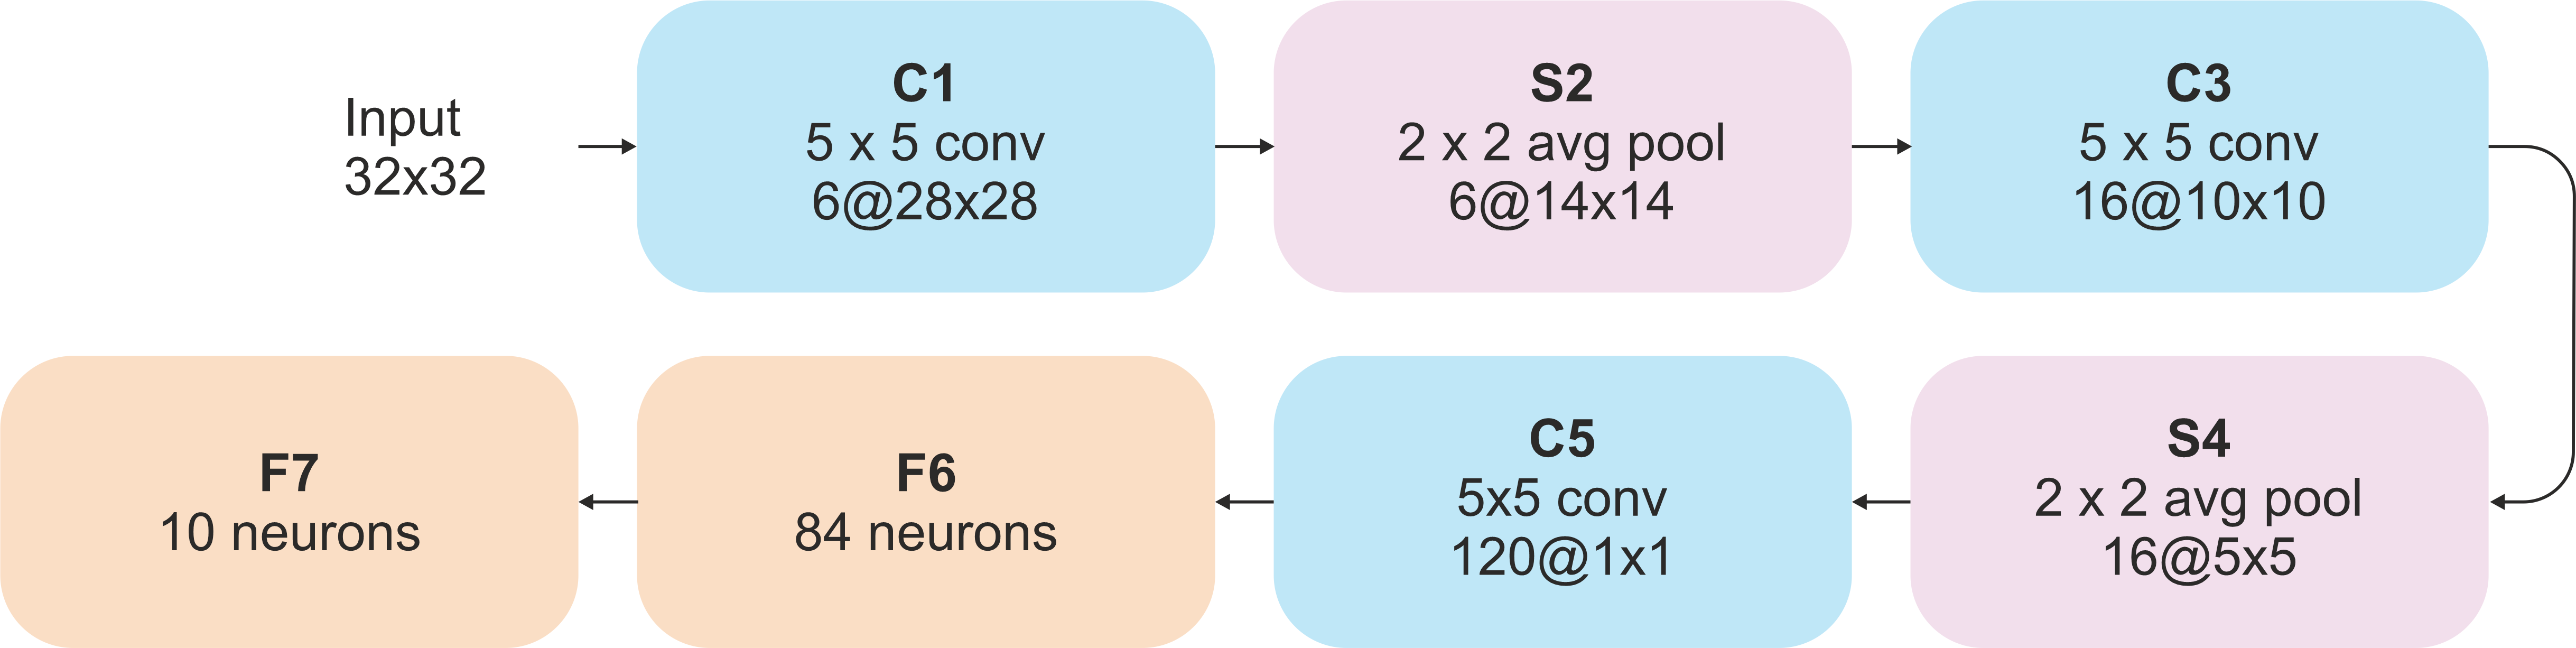
\includegraphics[width=.8\textwidth]{images/lenet.png}
    \caption{The LeNet architecture.}
    \label{img:lenet}
\end{figure}

\subsection{ResNet}

Residual neural network \cite{resnet2015} is a specific type of neural network that is constructed using residual blocks, which contain special residual connections. These blocks allow the network to be significantly deeper while also reducing the problem of vanishing gradient. Even with the increased depth, the residual network proved to be easier to optimize. After winning first place in ILSVRC \cite{ILSVRC} in 2015, the ResNet has become the default choice for using CNNs in practice. This is one of the reasons why we have decided to use it, to compare our network to state-of-the-art models.  

The topology of the residual block (Figure \ref{img:resblock0}) consists of two 3x3 convolutions, each followed by batch normalization and RELU activation. The main feature of the residual block is the residual connection, which adds the block input with the output directly before the last RELU activation. To be able to do the addition, the spatial size of the two convolutional layers needs to match the size of the input. The number of feature maps also needs to be the same, but this issue can be easily solved with a 1x1 convolution performed on the input. 

The concept of residual connections is based on the idea that stacking the layers to make the network deeper shouldn't reduce the performance, since we could just stack layers that don't change the value of the input data and we would get the same result. 
We will explain this using the Figure \ref{img:resblock0}. Let's assume that the mapping we want the network to learn is $f(x)$ with the input to the block denoted as $x$. With the residual block, the network only needs to learn the residual mapping $f(x) - x$, since the input $x$ will be added to the output. If the block needs to learn the identity mapping $f(x) = x$, it could simply just output zeros. This way, the block outputs the same data it received and therefore doesn't degrade the performance of the network with a deeper topology. 

\begin{figure}[h]
    \centering
    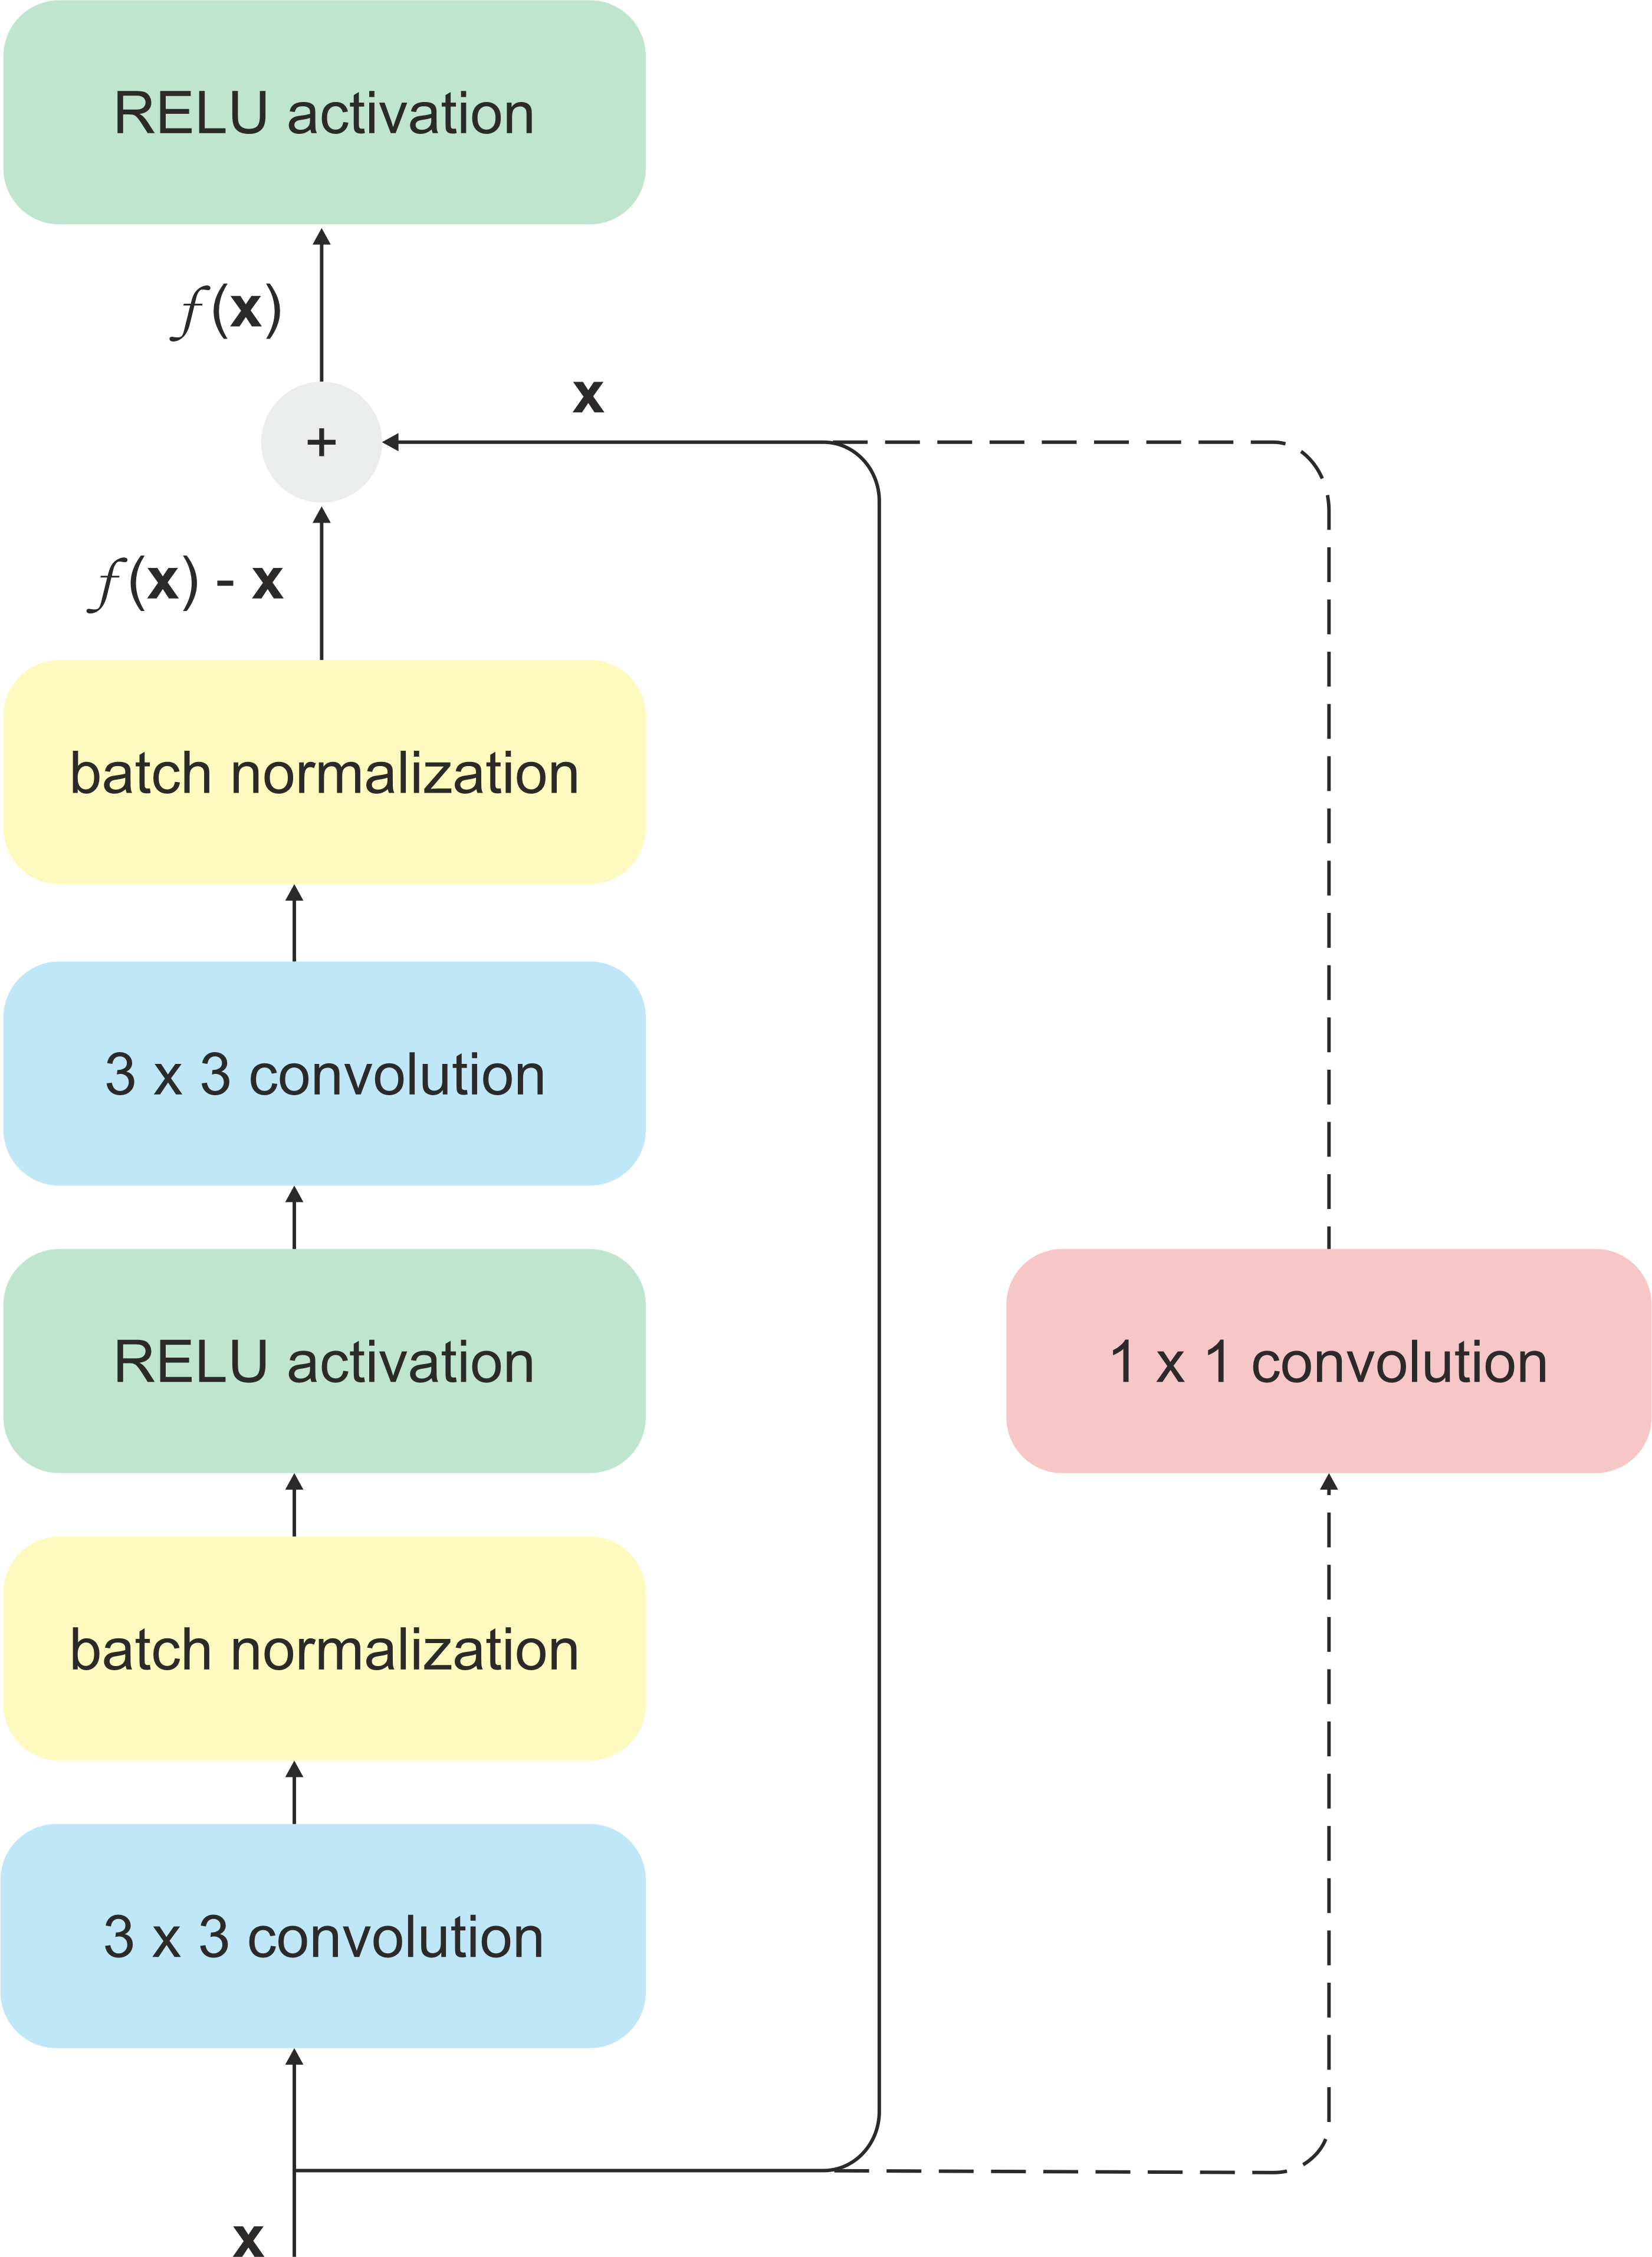
\includegraphics[width=0.4\textwidth]{images/residualblock.png}
    \caption{The structure of Resnet residual block.}
    \label{img:resblock0}
\end{figure}

By changing the number of filters and residual blocks, we can create different versions of ResNet models (ResNet-18, ResNet-152). In our work we are using ResNet-18 (Figure \ref{img:resnet18}) which consists of 18 layers. 


\begin{figure}[h]
    \centering
    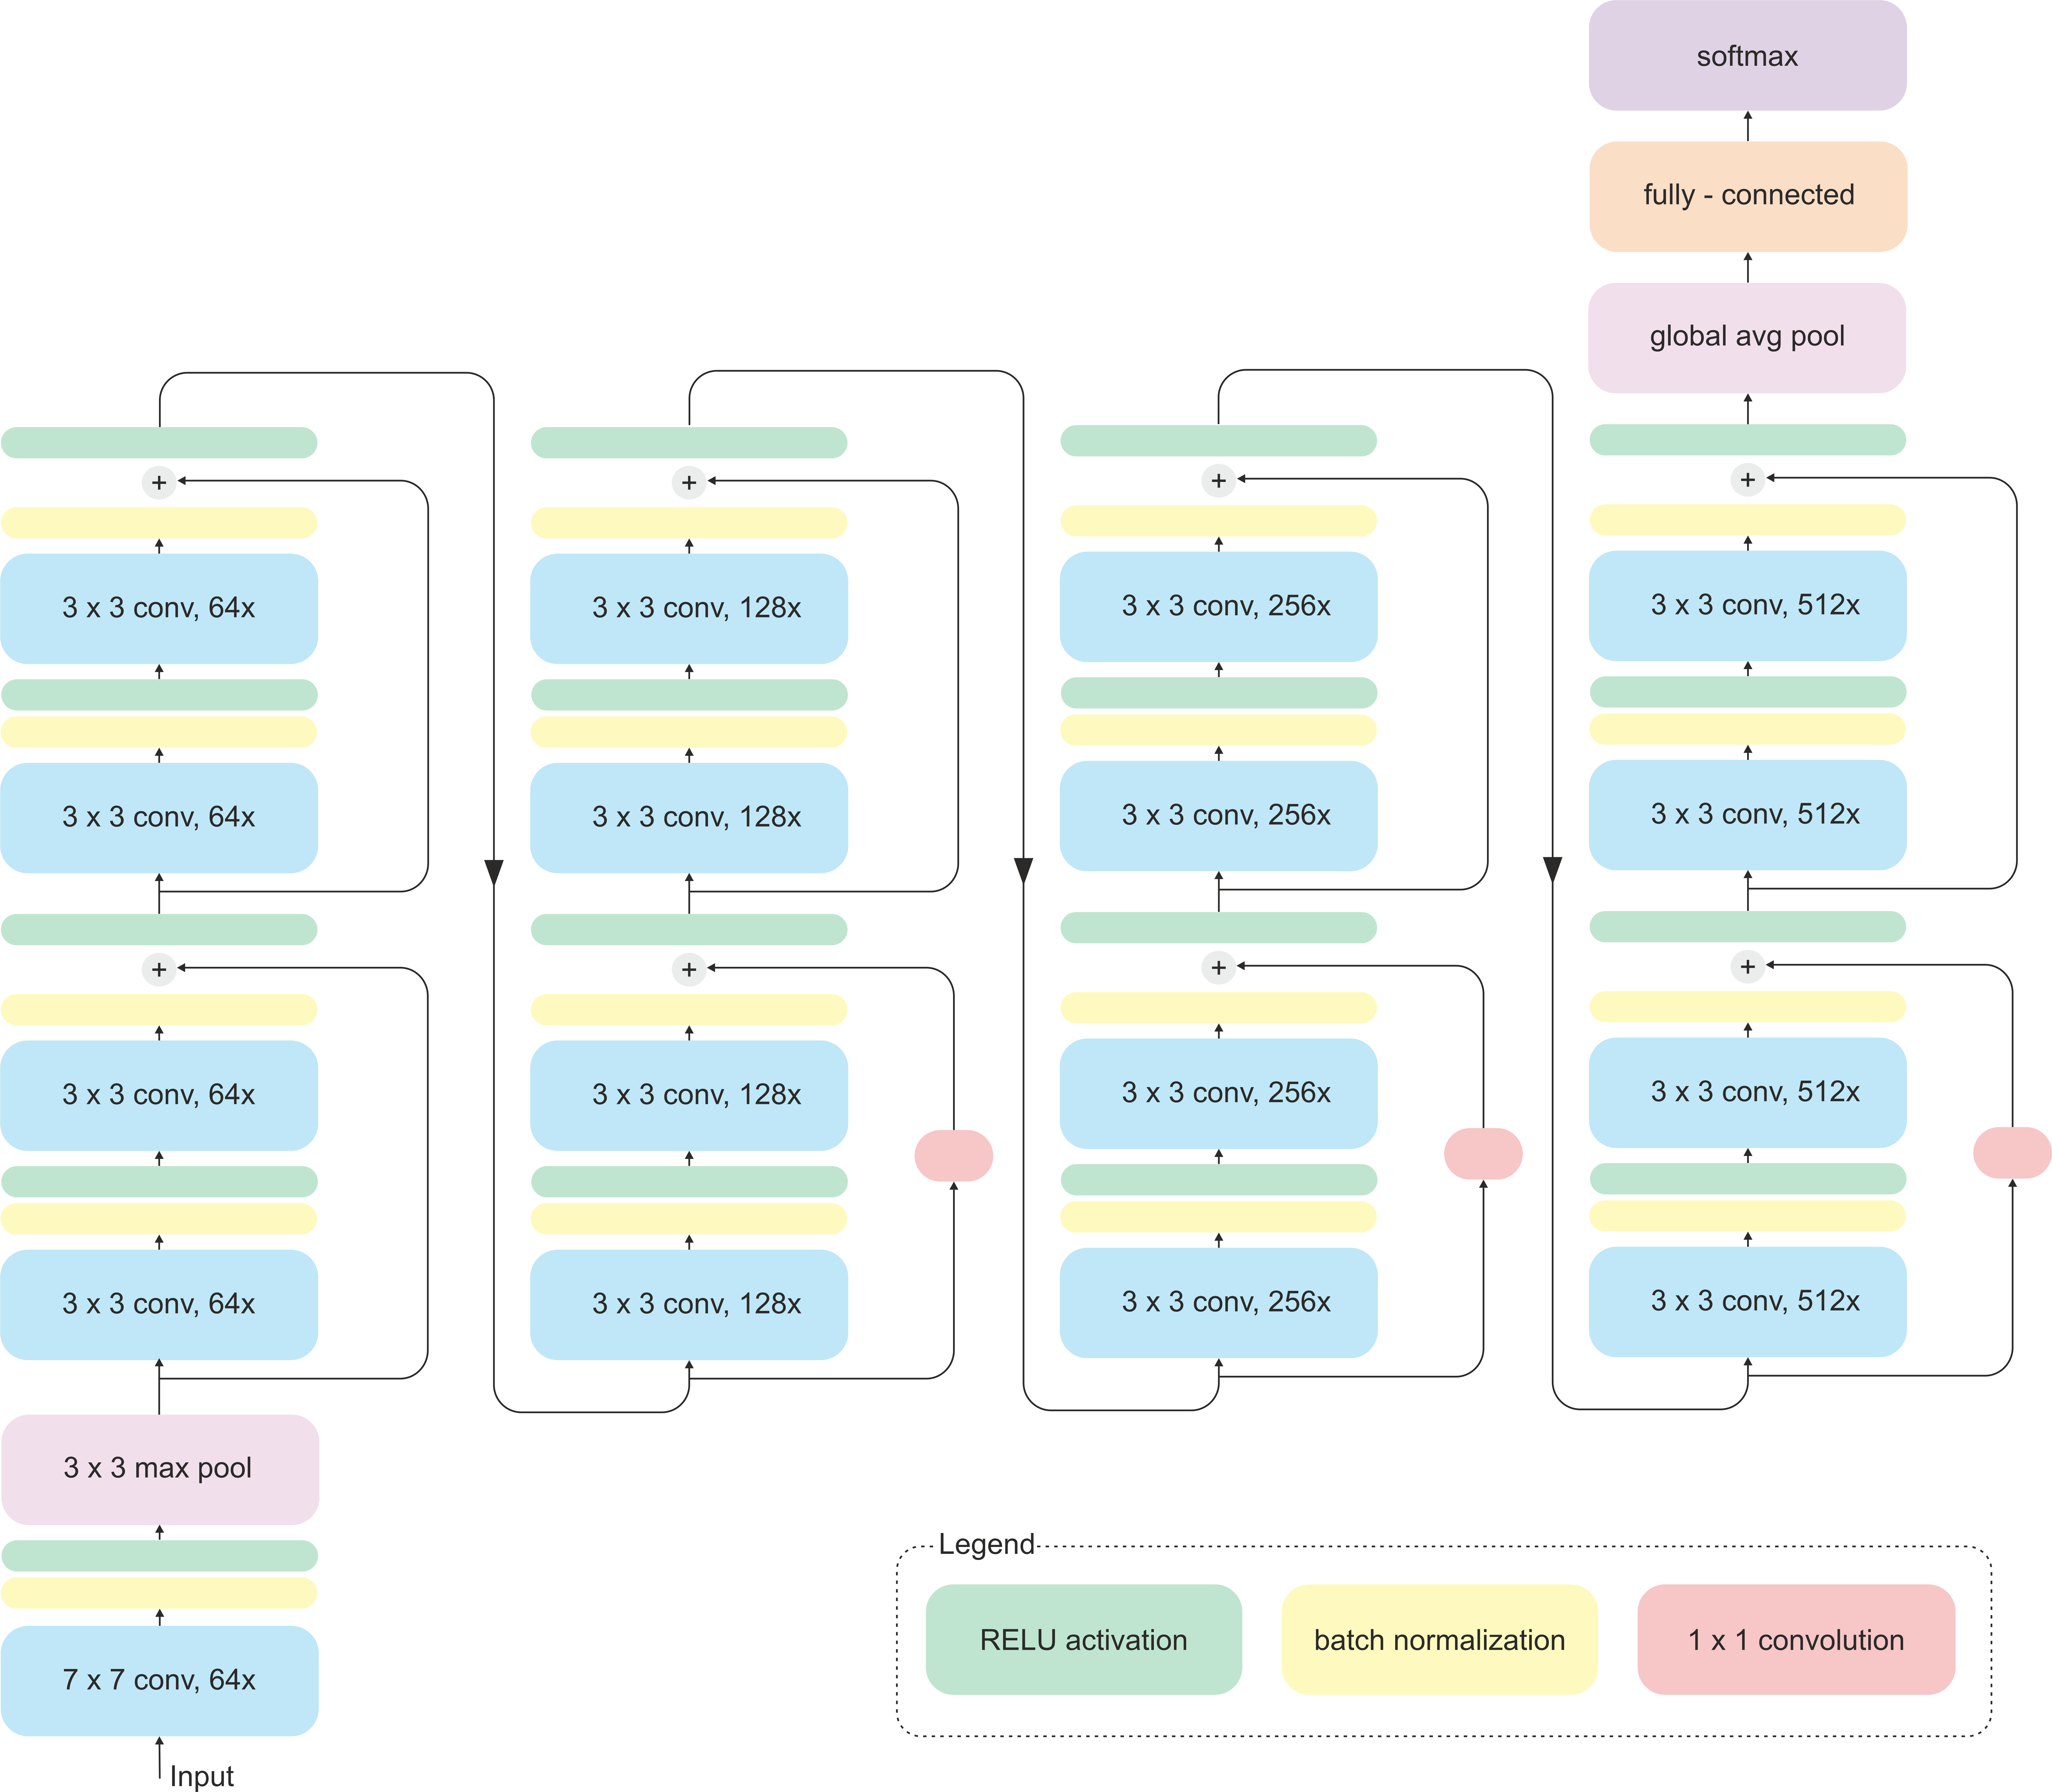
\includegraphics[width=0.8\textwidth]{images/resnet18.png}
    \caption{The ResNet-18 architecture.}
    \label{img:resnet18}
\end{figure}

\section{Data generator} \label{sec:sdgenerator}

For the training purposes of the network, we are developing a data generator. More specifically we are using the starGen and extending it to fit the needs of our thesis. The generator script is depicted in the Figure \ref{img:starGenActiviyDiagram}. 
In the beginning, the script reads the configuration file, which contains the general settings as well as settings for each generated object. The script generates multiple series and each series contains an arbitrary number of frames. The script supports the generation of stars, moving objects, clusters, and galaxies. Stars and galaxies are static in each frame, while clusters and moving objects move in consecutive frames. To make the images as realistic as possible, the script adds Gaussian and Poisson noise. It also supports defects such as hot pixels and cosmic rays. Other defects and noises are supported in a form of adding real BIAS, DARK and FLAT FIELD frames to the generated image. Other features of starGen include saving positions to TSV files, saving images in a form of FITS and PNG files, and plotting the images in the environment. It also includes the option to read the positions and brightness values of objects from the TSV file. 

\begin{figure}[h]
    \centering
    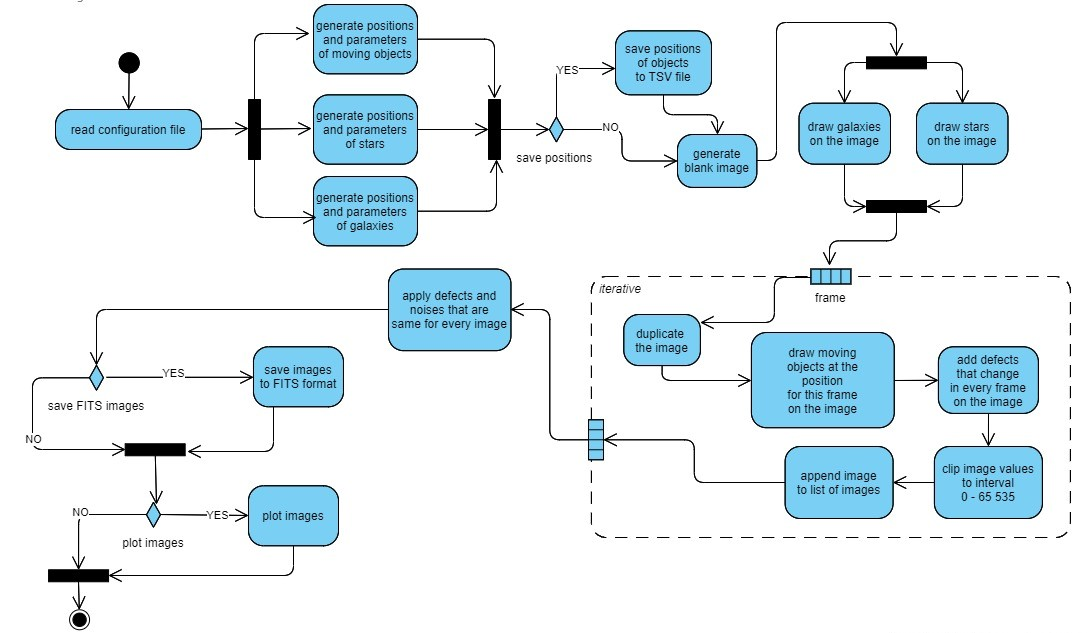
\includegraphics[width=\textwidth]{images/starGen2.jpg}
    \caption{Activity diagram of starGen script.}
    \label{img:starGenActiviyDiagram}
\end{figure}


\subsection{General settings}
General settings include image settings and also parameters of the generation itself. 
The script allows the user to set the number of generated series, the number of frames in the series, and the resolution of the generated image. Lots of parameters are binary indicators, that allow the user to choose whether he wants to save the images, plot the images and save the positions of objects. The user also defines the destination, where files are saved.  In case the positions of objects are read from the TSV file, the user is required to define the path to the file. For this approach to work, the number of frames in one series is not adjustable by the user but is determined by the file. 


\subsection{Supported objects}
As already mentioned, the generator supports multiple astronomical objects like stars, galaxies, moving objects, and clusters of moving objects. In this section, we will explain the parameters of each object. 

Note that all number parameters defined by the user are defined in the form of a range, where the user defines the minimum and maximum possible value and the script chooses a specific value from this interval. 

\subsubsection{Stars}
The generator allows user to define the number of generated stars using $count$, their maximal $brightness$, and $fwhm$ of their profile. Stars can be generated either as a point source, where the PSF is Gaussian or as a streak source, which consists of multiple overlapping Gaussians. This is determined by parameter $method$. In case the user chooses the stars to appear as streaks, additional parameters such as their rotation $alpha$ and $length$ need to be set. The rotation $alpha$ is anticlockwise and the values range from 0 to 360 degrees. The length of the streak is measured as half-length and the unit is $\sigma$ of the Gauss function. During one series, stars are static and they stay in the same position. All generated stars have the same $fwhm$, $alpha$ and $length$, while the $brightness$ differs. 

\subsubsection{Moving objects}
Similar to stars user can define the number of moving objects with parameter $count$, their $brightness$, $fwhm$, $method$ of appearance, with the same additional parameters $alpha$ and $length$. However, moving objects are not static and they change positions in consecutive frames. To adjust how much they move in frames, the additional parameter $speed$ was defined. The value of the $speed$ parameter is described as the percentage of the image traveled by the object in one series and it is used in the following manner: 

\begin{equation}
    \Delta = \frac{dim \cdot speed}{frames} 
\end{equation}

where $\Delta$ defines the traveled distance in pixels between two consecutive frames, $dim$ is the smaller dimension of the image, and $frames$ is the number of frames in one series. 

The direction in which the object moves is controlled by the rotation $alpha$ even if the moving object is a point source. The script supports generation of multiple moving objects and each will have different $brightness$, $fwhm$, $alpha$, $length$ and $speed$. 


\subsubsection{Clusters of moving objects}
Clusters are very similar to moving objects and have the same set of parameters. The only difference is that with moving objects when multiple objects are generated each object has different motion parameters ($speed$, $alpha$, and $length$). A cluster object allows multiple objects to have the same motion parameters and move the same way. The number of objects in one cluster is specified with the $objectCountPerCluster$ parameter and each object in the cluster has the same motion. The script supports the generation of multiple clusters with the parameter $count$.   

\subsubsection{Galaxies}
Similar to other objects, the script allows to generate multiple galaxies specifying their number by $count$. Elliptical galaxies have an inner core that is very bright, small, and concentrated. The outer part is larger in the area and the brightness is rapidly fading away from the core. The user can define the brightness of the inner core using the $brightness$ parameter. The brightness of the outer area is calculated using $brightnessFactor$ which defines the percentage of the $brightness$ and is used in the following manner: 

\begin{equation} \label{eq:brightnessGalaxy}
    b_a = brightnessFactor \cdot b_c
\end{equation}

where $b_a$ is the brightness of the outer area, and $b_c$ is the brightness of the core. 
Another parameters include $sigmaX$ and $sigmaY$ that define the variance of the outer area in x, y direction, and $sigmaFactor$ that describes the percentage of the variances for the inner core which is calculated as follows: 

\begin{equation} \label{eq:sigmaGalaxy}
    \begin{split}
        sigmaX_c = sigmaFactor \cdot sigmaX \\
        sigmaY_c = sigmaFactor \cdot sigmaY
    \end{split}
\end{equation}
where $sigmaX_c$, $sigmaY_c$ are variance of the inner core of the galaxy in the x,y direction. 
Lastly, the galaxy has its rotation which is defined by $alpha$ and contains values from 0 to 180 degrees. 


\subsection{Supported defects and noises}
To make images realistic, defects and noises that corrupt real astronomical images were added to the generator. 
This includes noises such as Gaussian noise and Poisson noise and defects like hot pixels and cosmic rays. We are aware that some noises and defects are missing. However, the data generator was not the primary focus of the thesis and was only a secondary tool to generate images for training purposes. Yet to make up for missing noises, we added the option to use real BIAS, DARK and FLAT FIELD frames in the generation. These real frames already include readout noise, bias voltage, dark current, dead columns, dust rings, vignette, and others (more info in Section \ref{sec:defects}). 

\subsubsection{Gaussian noise}
Gaussian noise is used to simulate the sky background noise. It is applied to each frame separately to keep the randomness in the images. The user can define the $mean$ and standard deviation ($std$) of the noise.

\subsubsection{Poisson noise}
Poisson noise is applied to each generated object to simulate the photons falling onto the chip. In the configuration file, the user can define if he wants to apply the Poisson noise using the $applyPoisson$ boolean parameter. 

\subsubsection{Hot pixels}
In the generation of hot pixels on the image, the user can set their $count$ and $brightness$. In generated series, hot pixels are static and stay at the same position in all frames. 

\subsubsection{Cosmic rays}
In the configuration file, the user can set the number of generated cosmic rays with $count$, as well as their $brightness$. In Section \ref{sec:defects} we mentioned three different types of cosmic rays: spots, tracks, and worms. Spots usually have fewer pixels than tracks and worms, which is why the user can define the number of pixels using $spotPixelCount$ for spots and $pixelCount$ for tracks and worms. Cosmic rays are generated randomly for each frame since in the real observations they occur randomly as well.

\subsubsection{BIAS, DARK, FLAT FIELD frames}
When using real frames, the user must define the path to the real images using parameter $dataDir$. Important to note, that the images must have the same dimensions as the generated image, or else it will not work correctly. The same real frames are applied to each frame after all objects are generated. First, we multiply the image with the values from the FLAT FIELD frame, which defines the pixel sensitivity. DARK and BIAS frames are added afterward. DARK frames usually already contain bias voltage, so we don't need to apply the BIAS frame.






% \chapter{Software design} \label{chap:softwaredesign}

In our work, we are implementing a system that can recognize the following astronomical objects present in the image: 

\begin{itemize}
    \item point source
    \item streak source
    \item streak source that is cut due to being on the edge of the image
    \item elliptical galaxy
    \item cosmic ray
    \item hot pixel
\end{itemize}

As mentioned before, the task of object recognition includes object localization and classification. Because we are using types of astronomical objects, that were not discussed in approaches in \ref{sec:spacerecognition}, we first want to access the possibility of using a neural network to correctly classify our objects into classes. For this reason, we omitted the object localization task. 

The designed network is thoroughly trained on a large amount of synthetic data. Data from real observations are later used to fine-tune the model. The performance of our network is also compared to the state-of-the-art ResNet-18 model. 


\section{Input data} \label{sec:inputdata}

Input data to our network are images in a form of FITS files. Each image contains only one astronomical object as depicted in the Figure \ref{fig:fitsreal3}. The size of the image is 50x50 pixels, as it was mentioned in \cite{Andreon2000} that it is the optimal size of the image for one object to be classified. 
Pixel values of the image are stored in 16 bits, which means that values range from 0 to 65 535. Although the images are in FITS format, we are only making use of the data block and the header is empty. 

In our work, we are using synthetic images as well as real ones. 
However, real images provided by the telescope in AGO have a resolution of 1024x1024 and capture the whole starfield. For us to be able to use these images, we needed to manually cut out 50x50 windows from them with just one astronomical object present. Some examples of such cutouts are shown in the Figure \ref{fig:fitsreal3}.  


\begin{figure}[!h]
   \centering
    \begin{subfigure}{.2\textwidth}
        \centering
        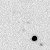
\includegraphics[width=\textwidth]{images/point.png}
        \label{fig:fitsreal3a}
        \caption{Point.}
    \end{subfigure}
    %\hfill
    \begin{subfigure}{.2\textwidth}
        \centering
        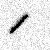
\includegraphics[width=\textwidth]{images/line2.png}
        \label{fig:fitsreal3b}
        \caption{Streak.}
    \end{subfigure}
    %\hfill
    \begin{subfigure}{.2\textwidth}
        \centering
        
\includegraphics[width=\textwidth]{images/cutline.png}
        \label{fig:fitsreal3c}
        \caption{Cut Streak.}
    \end{subfigure}
    %\hfill
    
    \vspace*{4mm}
    
    \begin{subfigure}{.2\textwidth}
        \centering
        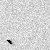
\includegraphics[width=\textwidth]{images/cosmicray.png}
        \label{fig:fitsreal3d}
        \caption{Cosmic ray.}
    \end{subfigure}
    %\hfill
    \begin{subfigure}{.2\textwidth}
        \centering
        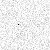
\includegraphics[width=\textwidth]{images/hotpixel.png}
        \label{fig:fitsreal3e}
        \caption{Hot pixel.}
    \end{subfigure}
    %\hfill
    \begin{subfigure}{.2\textwidth}
        \centering
        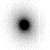
\includegraphics[width=\textwidth]{images/galaxy.png}
        \label{fig:fitsreal3f}
        \caption{Galaxy.}
    \end{subfigure}
    %\hfill
    \caption{Examples of 50x50 pixel cutouts from real images.}
    \label{fig:fitsreal3}
\end{figure}

\section{Recognition system}

%	ake classy tam budu (samostatny dataset, trainer, tester)
% potom opiseme nejaku strukturu siete
% ze ju programuje v pytorchi a mozno povedat ze aku verziu cudy a nejake packages
% mozno class diagram 
% programovacie prostredie python, pytorch, verzia cudy
% parametre mojho pocitaca na ktory to deploynem


%outline:
%uvod
%    - ze je to skript v pythone
%    - ze pouzivam nejake packages zname
%    - ze je to deploynute tam a tam
%project structure
%    - kazdu triedu opisat 
%    - class diagram
%    - deklaraciu CNN

The system is implemented in Python in a form of Jupyter notebook. The network is implemented using Pytorch library with Cuda 11.3. Other useful packages include: numpy, scipy, matplotlib, sklearn, astropy, etc. 


\subsection{Deployment}
The training of the network is running on the desktop computer with Microsoft Windows 10 Pro operating system. The hardware consists of the following:
\begin{itemize}
    \item Intel(R) Core(TM) i7-6700 CPU @ 3.40GHz, 3401 MHz, with 4 cores and 8 logical processors 
    \item NVIDIA GeForce GTX 1050 Ti
    \item 16GB of RAM memory
\end{itemize}

\subsection{Project structure}

As mentioned before the system is written in the Jupyter notebook. This allows us to train multiple times, without having to load the data every time. It is also easier to configure the parameters of the network and see the progress in real-time. 

The structure of the notebook is divided into multiple cells to allow us to run the specific cell we need without having to run redundant operations. To improve the quality of the script we have created multiple helpful classes, depicted in the Figure \ref{img:networkClass}: 

\begin{itemize}
    \item \textbf{MyDataLoader} \\
    The class loads all training, validation, and testing data from folders and parses them into the Dataset class. It uses the name of the folders to assign labels to each image.
    
    \item \textbf{FITSDataset} \\
    The class implements torch.utils.data.Dataset class and loads FITS images into tensors. It also provides an option to pre-process data before loading them into tensors. 
    
    \item \textbf{DataAugmentation} \\
    Implements data augmentation techniques explained in the Section \ref{sec:parametersNetwork}. 
    
    \item \textbf{MyCNN} \\
    Contains a declaration of each layer of the convolutional neural network. Implements torch.nn.Module class. 
    
    \item \textbf{EarlyStopping} \\
    Performs the early stopping technique described in the Section \ref{sec:parametersNetwork}. 
    
    \item \textbf{Visualizer} \\
    Plots the evolution of loss and accuracy during training. The plotted images are saved as JPEG files in the defined destination folder. 
    
    \item \textbf{Trainer} \\
    The class implements the training and validation of the network. It contains methods for forward and backward pass of the network. It stores the training and validation loss and observes its progress for the early stopping algorithm. 
    
    \item \textbf{Tester} \\
    Evaluates the network using testing data. It outputs the accuracy, recall, and precision of the trained model as well as plots confusion matrices. Moreover, it saves images that were wrongly classified during evaluation. 
\end{itemize}

\begin{figure}[h]
    \centering
    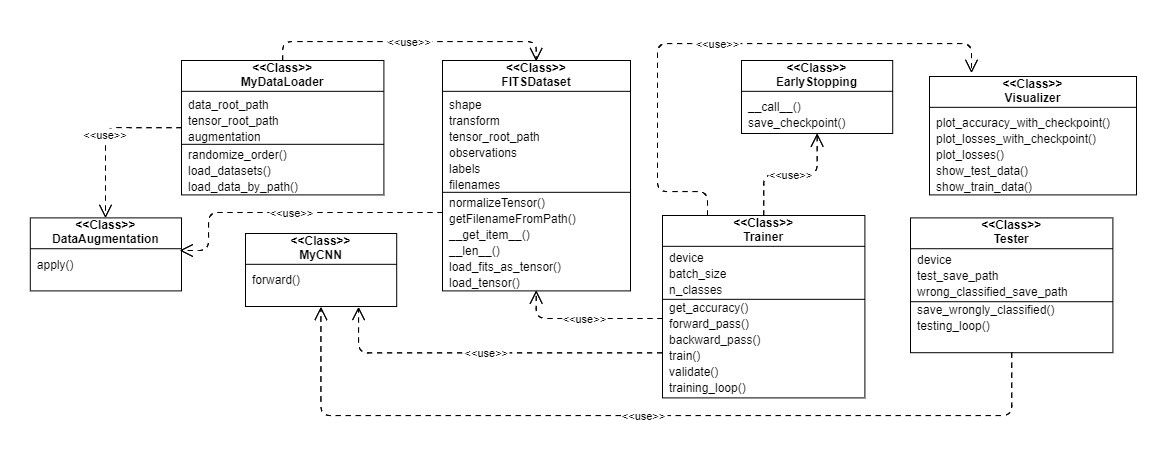
\includegraphics[width=\textwidth]{images/classDiagramNetwork.png}
    \caption{Class diagram of the recognition system.}
    \label{img:networkClass}
\end{figure}


\section{Data generator} \label{sec:sdgenerator}

For the training purposes of the network, we are developing a data generator. More specifically we are using the starGen and extending it to fit the needs of our thesis. The generator script is depicted in the Figure \ref{img:starGenActiviyDiagram}. 
In the beginning, the script reads the configuration file, which contains the general settings as well as settings for each generated object. The script generates multiple series and each series contains an arbitrary number of frames. The script supports the generation of stars, moving objects, clusters, and galaxies. Stars and galaxies are static in each frame, while clusters and moving objects move in consecutive frames. To make the images as realistic as possible, the script adds Gaussian and Poisson noise. It also supports defects such as hot pixels and cosmic rays. Other defects and noises are supported in a form of adding real BIAS, DARK and FLAT FIELD frames to the generated image. Other features of starGen include saving positions to TSV files, saving images in a form of FITS and PNG files, and plotting the images in the environment. It also includes the option to read the positions and brightness values of objects from the TSV file. 

\begin{figure}[h]
    \centering
    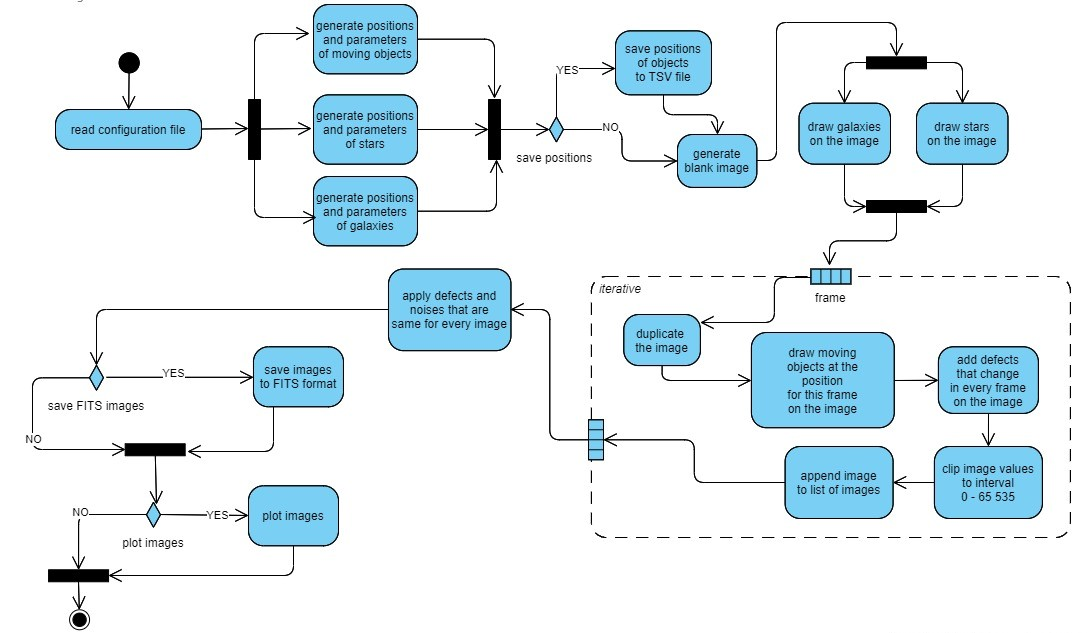
\includegraphics[width=\textwidth]{images/starGen2.jpg}
    \caption{Activity diagram of starGen script.}
    \label{img:starGenActiviyDiagram}
\end{figure}


\subsection{General settings}
General settings include image settings and also parameters of the generation itself. 
The script allows the user to set the number of generated series, the number of frames in the series, and the resolution of the generated image. Lots of parameters are binary indicators, that allow the user to choose whether he wants to save the images, plot the images and save the positions of objects. The user also defines the destination, where files are saved.  In case the positions of objects are read from the TSV file, the user is required to define the path to the file. For this approach to work, the number of frames in one series is not adjustable by the user but is determined by the file. 


\subsection{Supported objects}
As already mentioned, the generator supports multiple astronomical objects like stars, galaxies, moving objects, and clusters of moving objects. In this section, we will explain the parameters of each object. 

Note that all number parameters defined by the user are defined in the form of a range, where the user defines the minimum and maximum possible value and the script chooses a specific value from this interval. 

\subsubsection{Stars}
The generator allows user to define the number of generated stars using $count$, their maximal $brightness$, and $fwhm$ of their profile. Stars can be generated either as a point source, where the PSF is Gaussian or as a streak source, which consists of multiple overlapping Gaussians. This is determined by parameter $method$. In case the user chooses the stars to appear as streaks, additional parameters such as their rotation $alpha$ and $length$ need to be set. The rotation $alpha$ is anticlockwise and the values range from 0 to 360 degrees. The length of the streak is measured as half-length and the unit is $\sigma$ of the Gauss function. During one series, stars are static and they stay in the same position. All generated stars have the same $fwhm$, $alpha$ and $length$, while the $brightness$ differs. 

\subsubsection{Moving objects}
Similar to stars user can define the number of moving objects with parameter $count$, their $brightness$, $fwhm$, $method$ of appearance, with the same additional parameters $alpha$ and $length$. However, moving objects are not static and they change positions in consecutive frames. To adjust how much they move in frames, the additional parameter $speed$ was defined. The value of the $speed$ parameter is described as the percentage of the image traveled by the object in one series and it is used in the following manner: 

\begin{equation}
    \Delta = \frac{dim \cdot speed}{frames} 
\end{equation}

where $\Delta$ defines the traveled distance in pixels between two consecutive frames, $dim$ is the smaller dimension of the image, and $frames$ is the number of frames in one series. 

The direction in which the object moves is controlled by the rotation $alpha$ even if the moving object is a point source. The script supports generation of multiple moving objects and each will have different $brightness$, $fwhm$, $alpha$, $length$ and $speed$. 


\subsubsection{Clusters of moving objects}
Clusters are very similar to moving objects and have the same set of parameters. The only difference is that with moving objects when multiple objects are generated each object has different motion parameters ($speed$, $alpha$, and $length$). A cluster object allows multiple objects to have the same motion parameters and move the same way. The number of objects in one cluster is specified with the $objectCountPerCluster$ parameter and each object in the cluster has the same motion. The script supports the generation of multiple clusters with the parameter $count$.   

\subsubsection{Galaxies}
Similar to other objects, the script allows to generate multiple galaxies specifying their number by $count$. Elliptical galaxies have an inner core that is very bright, small, and concentrated. The outer part is larger in the area and the brightness is rapidly fading away from the core. The user can define the brightness of the inner core using the $brightness$ parameter. The brightness of the outer area is calculated using $brightnessFactor$ which defines the percentage of the $brightness$ and is used in the following manner: 

\begin{equation} \label{eq:brightnessGalaxy}
    b_a = brightnessFactor \cdot b_c
\end{equation}

where $b_a$ is the brightness of the outer area, and $b_c$ is the brightness of the core. 
Another parameters include $sigmaX$ and $sigmaY$ that define the variance of the outer area in x, y direction, and $sigmaFactor$ that describes the percentage of the variances for the inner core which is calculated as follows: 

\begin{equation} \label{eq:sigmaGalaxy}
    \begin{split}
        sigmaX_c = sigmaFactor \cdot sigmaX \\
        sigmaY_c = sigmaFactor \cdot sigmaY
    \end{split}
\end{equation}
where $sigmaX_c$, $sigmaY_c$ are variance of the inner core of the galaxy in the x,y direction. 
Lastly, the galaxy has its rotation which is defined by $alpha$ and contains values from 0 to 180 degrees. 


\subsection{Supported defects and noises}
To make images realistic, defects and noises that corrupt real astronomical images were added to the generator. 
This includes noises such as Gaussian noise and Poisson noise and defects like hot pixels and cosmic rays. We are aware that some noises and defects are missing. However, the data generator was not the primary focus of the thesis and was only a secondary tool to generate images for training purposes. Yet to make up for missing noises, we added the option to use real BIAS, DARK and FLAT FIELD frames in the generation. These real frames already include readout noise, bias voltage, dark current, dead columns, dust rings, vignette, and others (more info in Section \ref{sec:defects}). 

\subsubsection{Gaussian noise}
Gaussian noise is used to simulate the sky background noise. It is applied to each frame separately to keep the randomness in the images. The user can define the $mean$ and standard deviation ($std$) of the noise.

\subsubsection{Poisson noise}
Poisson noise is applied to each generated object to simulate the photons falling onto the chip. In the configuration file, the user can define if he wants to apply the Poisson noise using the $applyPoisson$ boolean parameter. 

\subsubsection{Hot pixels}
In the generation of hot pixels on the image, the user can set their $count$ and $brightness$. In generated series, hot pixels are static and stay at the same position in all frames. 

\subsubsection{Cosmic rays}
In the configuration file, the user can set the number of generated cosmic rays with $count$, as well as their $brightness$. In Section \ref{sec:defects} we mentioned three different types of cosmic rays: spots, tracks, and worms. Spots usually have fewer pixels than tracks and worms, which is why the user can define the number of pixels using $spotPixelCount$ for spots and $pixelCount$ for tracks and worms. Cosmic rays are generated randomly for each frame since in the real observations they occur randomly as well.

\subsubsection{BIAS, DARK, FLAT FIELD frames}
When using real frames, the user must define the path to the real images using parameter $dataDir$. Important to note, that the images must have the same dimensions as the generated image, or else it will not work correctly. The same real frames are applied to each frame after all objects are generated. First, we multiply the image with the values from the FLAT FIELD frame, which defines the pixel sensitivity. DARK and BIAS frames are added afterward. DARK frames usually already contain bias voltage, so we don't need to apply the BIAS frame.











%%% useful webpages
% https://ml-cheatsheet.readthedocs.io/en/latest/regularization.html#data-augmentation
% https://d2l.ai/chapter_computational-performance/index.html

% \chapter{Implementation}
\label{chap:implementation}

This chapter focuses on the implementation aspects of the KSA Dashboard. 

\section{Parser}
\label{sec:parser}

To make the product extendable, parser service defines a common interface for all security scanner parsers and provides a common definition of vulerabilty and misconfiguration using Golang structures. Listing~\ref{lst:parser-interface} shows a code snippet of the definition. Golang does not support objects and classes in the traditional sense. Instead, it uses interfaces: any structure that implements the methods of the interface is considered to satisfy that interface.

\begin{lstlisting}[language=Go, caption={[A common interface for parsers] A common interface for parsers.}, label={lst:parser-interface}]
    /* Parser defines a common interface 
    for all security scanner parsers */
    type Parser interface {
        Parse(filePath string) ([]Vulnerability, 
            []Misconfiguration, error)
        GetResults() interface{}
        GetVulnerabilities() []Vulnerability
        GetMisconfigurations() []Misconfiguration
    }
\end{lstlisting}

We parse the JSON reports using the standard Go module \lstinline{encoding/json}. However, the structure of those reports varies significantly and sometimes is very complex. Some reports, like the ones produced by Kube-bench for instance, are missing some fields. Kube-bench does not specify the severity of its findings, neither it specifies the target. In this case we have to use default values: we set severity to \textbf{HIGH}, for example. Additionally, Kube-bench sets status to \textbf{WARN} for manual checks and those have to be remapped onto \textbf{MANUAL} to be consistent with the Prowler's notation.

Go's \lstinline{net/http} library is used to expose a number of endpoints for other services to use. As the server creates a new goroutine for each incoming HTTP request, we have to be careful with our data. Instances of our parsers are static and shared by those goroutines. That is why each instance has a mutex, that is locked whenever a critical operation is performed on the data and unlocked afterwards.

In order to extend the Parser with a new tool, there are three things to be considered:
\begin{enumerate}[noitemsep]
    \item A new implementation of the parser interface (see Listing~\ref{lst:parser-interface}) should be defined. It must have \lstinline{Parse()} method, which would define parsing process for the scanner.
    \item This implementation should be added to the parser initialization inside the main function.
    \item Parser should be added to the database.
\end{enumerate}
\section{Aggregator}
\label{sec:aggregator}

Aggregator service defines a common interface for all security scanner runners and provides a common interface for job tracking. Listing~\ref{lst:runner-interface} shows a code snippet of the definition.

\begin{lstlisting}[language=Go, caption={[A common inteface for runners] A common inteface for runners.}, label={lst:runner-interface}]
    /* Runner defines a common interface 
    for all security scanner runners */
    type Runner interface {
        Run() error
        GetStatus() JobStatus
        CleanUp() error
        Watch(*sql.DB) (int, string)
    }
    
    type JobRunner struct {
        clientset   kubernetes.Interface
        namespace   string
        jobName     string
        scannerName string
        fileName    string
    }
\end{lstlisting}

Aggregator uses Kubernetes API to create and delete jobs and watch for their completion. Each runner is provided with the same Kubernetes clientset. It is a set of generated Go clients that allow us to interact with the Kubernetes API programmatically. It handles authentication, API requests, version negotiation, and resource management. Runner then defines a job as a Golang struct and sends it to the Kubernetes API for creation.

To extend Aggregator with a new scanner, the following steps should be considered:
\begin{enumerate}[noitemsep,nosep]
    \item If the scanner does not provide a Docker image, a custom Docker image should be defined and built.
    \item A new Runner implementation should be created. \lstinline{Run()} method should define and run the Kubernetes job for the scanner.
    \item Runner should be initiated inside the main Go function.
\end{enumerate}
\section{Dashboard}
\label{sec:dashboard}

KSA dashboard is, perhaps, the most complex component of all. We are using NextJS framework for the development. The application's code is broken down into 10 custom ReactJS components and defines 8 new types. We mostly use client components, only the API components run on the server side of the NodeJS application. The whole user experience is based on the \lstinline{useEffect} and \lstinline{useState} React functions, that reload data from the backend upon changes in the selected filters or search query. Additionally, community-made Lucide React icons are used to enhance user experience.

Figure~\ref{img:ksa-dashboard-ui} displays the dashboard interface. Top side of the dashboard is reserved for the filters, action buttons and search panel. Upon selecting the scanner and item type (Vulnerability or Misconfiguration), user are able to choose from the available reports to load the items. When ``All scanners'' is selected, dashboard fetches and displays misconfigurations or vulnerabilites from the latest reports (if such exist) generated by all scanners. First button on the action bar triggers a new scan for the selected scanner. Second button allows to download a JSON report, which includes all of the displayed items. Third and fourth buttons delete or resolve all of the filtered items, respectively. That is, users are able to filter items by a keyword and then delete or resolve all of them at once. This is very useful when, for instance, we are bound by a specific Java version by the contract with the customer. Therefore, we, perhaps, would want to mark all of the vulnerabilites which are filtered by the ``Java'' keyword as resolved.

\begin{figure}[!hbt]
	\begin{center}
		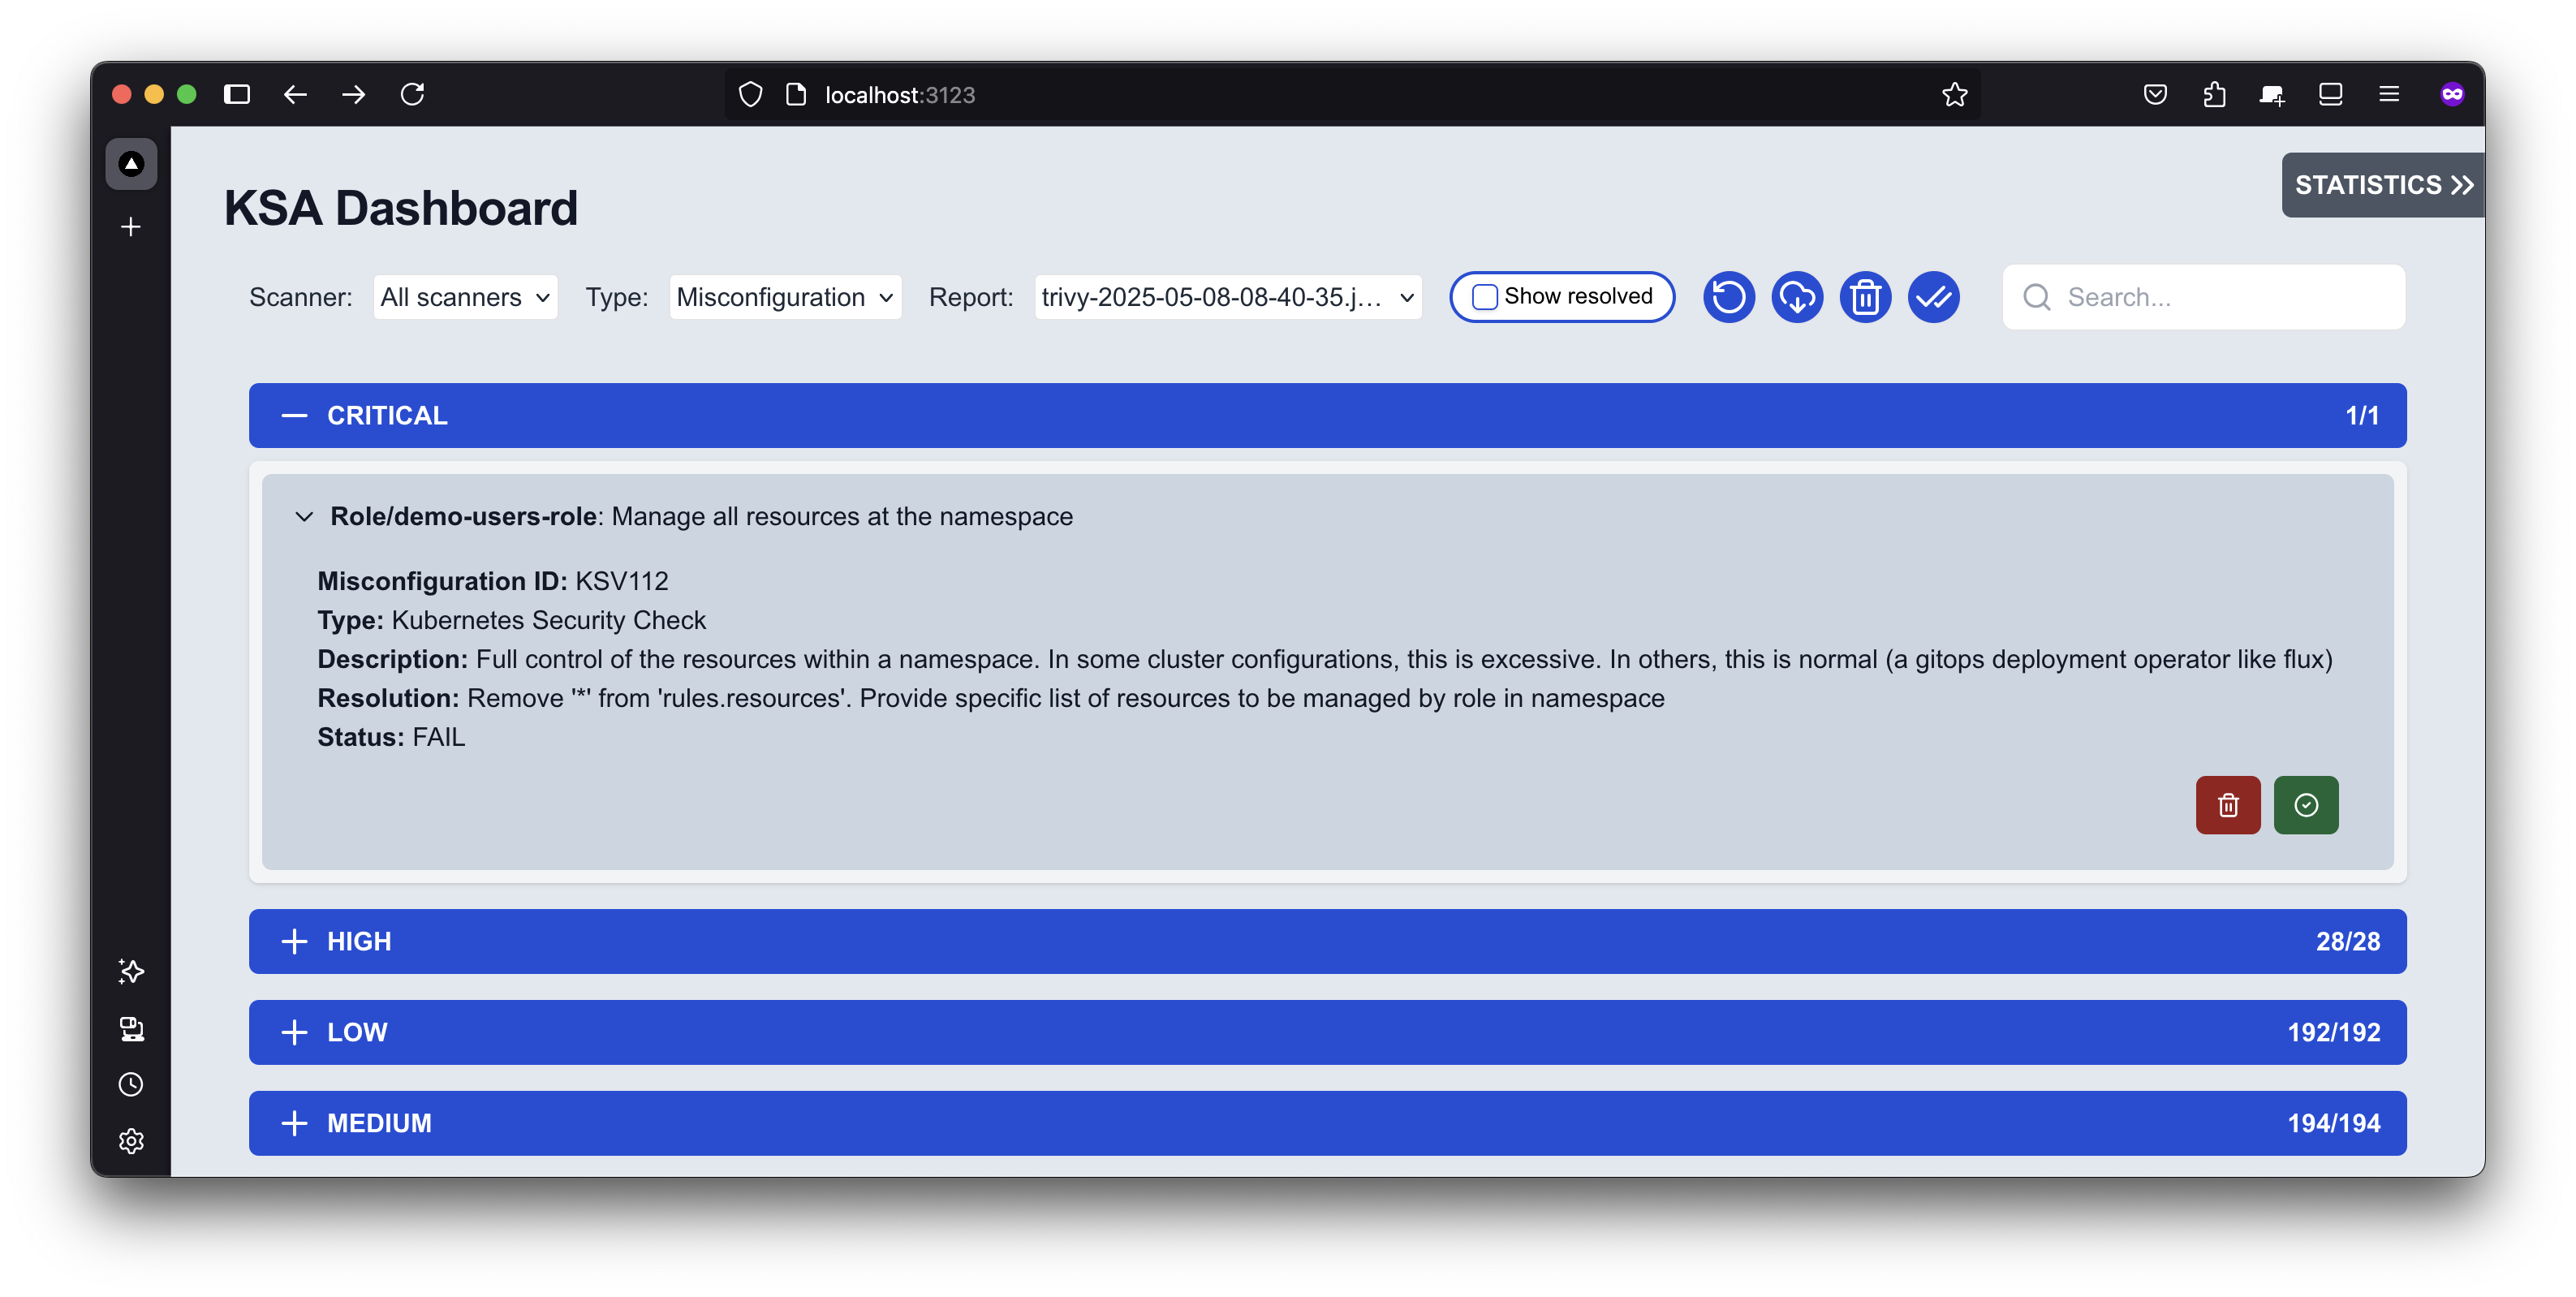
\includegraphics[width=0.9\textwidth]{images/ksa-dashboard-ui.png}
        \caption{User interface of the KSA dashboard.}
		\label{img:ksa-dashboard-ui}
	\end{center}
\end{figure}

The space below the panel is occupied by the list of the security threats. They are collapsed under different categories. Each item can be then also opened to examine the details, such as misconfiguration identifier, type, description, resolution and status. Item titles usually also include the target resource, where the misconfiguration was found.

In the top right corner of the dashboard is a \textbf{STATISTICS} button that provides some information on the most recent scan results in graphical format as shown below in Fig~\ref{img:ksa-dashboard-statistics}.

\begin{figure}[!hbt]
	\begin{center}
		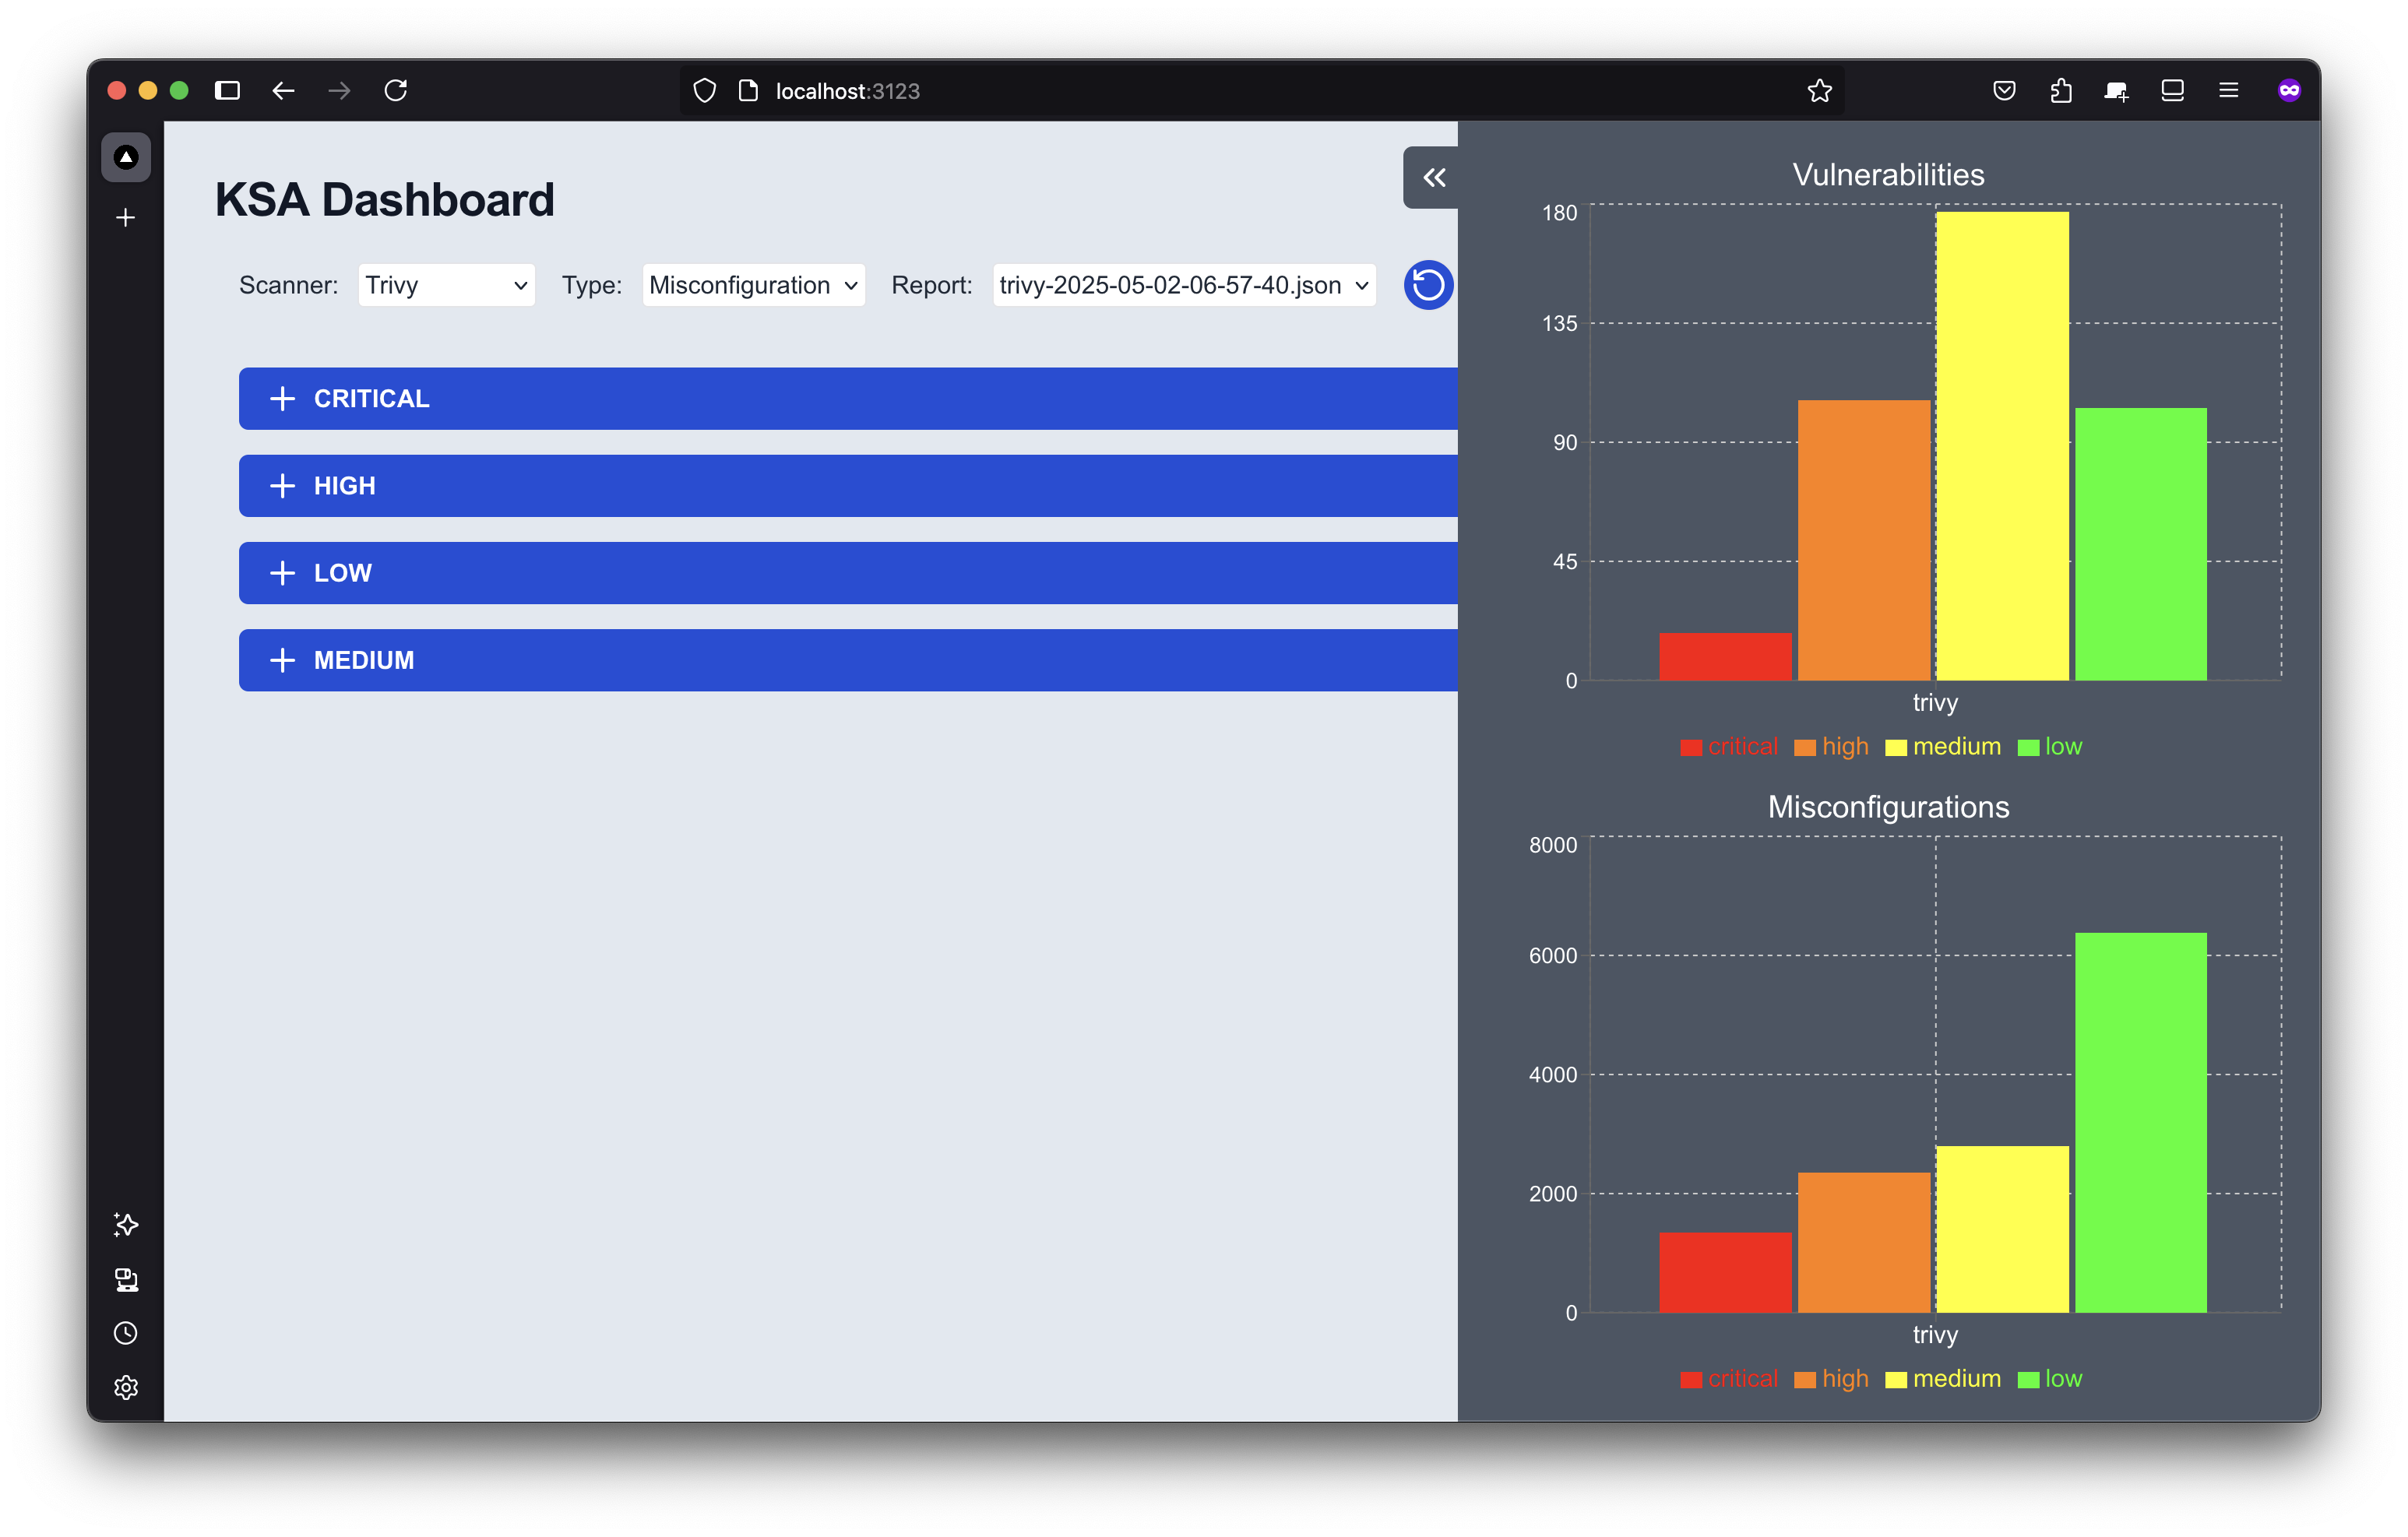
\includegraphics[width=0.9\textwidth]{images/ksa-dashboard-statistics.png}
        \caption{Statistics on the KSA dashboard.}
		\label{img:ksa-dashboard-statistics}
	\end{center}
\end{figure}
% \chapter{Data generation}

In this chapter, we explain how each object in the starGen script is generated. We compare 3D profiles between real and synthetic objects to demonstrate the fidelity of our generator to a real case scenario. We also present examples of each synthetic object and how each parameter affects its appearance. Finally, we explain how synthetic images were generated for the training dataset, and define the parameters used for the generation. 

\subsection{Supported objects}
As already mentioned, the generator supports multiple astronomical objects like stars, galaxies, moving objects, and clusters of moving objects. In this section, we will explain the parameters of each object. 

Note that all number parameters defined by the user are defined in the form of a range, where the user defines the minimum and maximum possible value and the script chooses a specific value from this interval. 

\subsubsection{Stars}
The generator allows user to define the number of generated stars using $count$, their maximal $brightness$, and $fwhm$ of their profile. Stars can be generated either as a point source, where the PSF is Gaussian or as a streak source, which consists of multiple overlapping Gaussians. This is determined by parameter $method$. In case the user chooses the stars to appear as streaks, additional parameters such as their rotation $alpha$ and $length$ need to be set. The rotation $alpha$ is anticlockwise and the values range from 0 to 360 degrees. The length of the streak is measured as half-length and the unit is $\sigma$ of the Gauss function. During one series, stars are static and they stay in the same position. All generated stars have the same $fwhm$, $alpha$ and $length$, while the $brightness$ differs. 

\subsubsection{Moving objects}
Similar to stars user can define the number of moving objects with parameter $count$, their $brightness$, $fwhm$, $method$ of appearance, with the same additional parameters $alpha$ and $length$. However, moving objects are not static and they change positions in consecutive frames. To adjust how much they move in frames, the additional parameter $speed$ was defined. The value of the $speed$ parameter is described as the percentage of the image traveled by the object in one series and it is used in the following manner: 

\begin{equation}
    \Delta = \frac{dim \cdot speed}{frames} 
\end{equation}

where $\Delta$ defines the traveled distance in pixels between two consecutive frames, $dim$ is the smaller dimension of the image, and $frames$ is the number of frames in one series. 

The direction in which the object moves is controlled by the rotation $alpha$ even if the moving object is a point source. The script supports generation of multiple moving objects and each will have different $brightness$, $fwhm$, $alpha$, $length$ and $speed$. 


\subsubsection{Clusters of moving objects}
Clusters are very similar to moving objects and have the same set of parameters. The only difference is that with moving objects when multiple objects are generated each object has different motion parameters ($speed$, $alpha$, and $length$). A cluster object allows multiple objects to have the same motion parameters and move the same way. The number of objects in one cluster is specified with the $objectCountPerCluster$ parameter and each object in the cluster has the same motion. The script supports the generation of multiple clusters with the parameter $count$.   

\subsubsection{Galaxies}
Similar to other objects, the script allows to generate multiple galaxies specifying their number by $count$. Elliptical galaxies have an inner core that is very bright, small, and concentrated. The outer part is larger in the area and the brightness is rapidly fading away from the core. The user can define the brightness of the inner core using the $brightness$ parameter. The brightness of the outer area is calculated using $brightnessFactor$ which defines the percentage of the $brightness$ and is used in the following manner: 

\begin{equation} \label{eq:brightnessGalaxy}
    b_a = brightnessFactor \cdot b_c
\end{equation}

where $b_a$ is the brightness of the outer area, and $b_c$ is the brightness of the core. 
Another parameters include $sigmaX$ and $sigmaY$ that define the variance of the outer area in x, y direction, and $sigmaFactor$ that describes the percentage of the variances for the inner core which is calculated as follows: 

\begin{equation} \label{eq:sigmaGalaxy}
    \begin{split}
        sigmaX_c = sigmaFactor \cdot sigmaX \\
        sigmaY_c = sigmaFactor \cdot sigmaY
    \end{split}
\end{equation}
where $sigmaX_c$, $sigmaY_c$ are variance of the inner core of the galaxy in the x,y direction. 
Lastly, the galaxy has its rotation which is defined by $alpha$ and contains values from 0 to 180 degrees. 


\section{Generated data}
%We have shown how each object is generated and examples of images with just one object. 

The starGen script can generate full-frame series of images with multiple various objects and defects. With the right settings of the configuration file, the system can produce various scenarios mentioned in the Section \ref{sec:scenarios}. Examples of such generated images are shown in the Figure \ref{fig:stargenfullframe}. 

\begin{figure}[!h]
\centering
    \begin{subfigure}[t]{.4\textwidth}
        \centering
        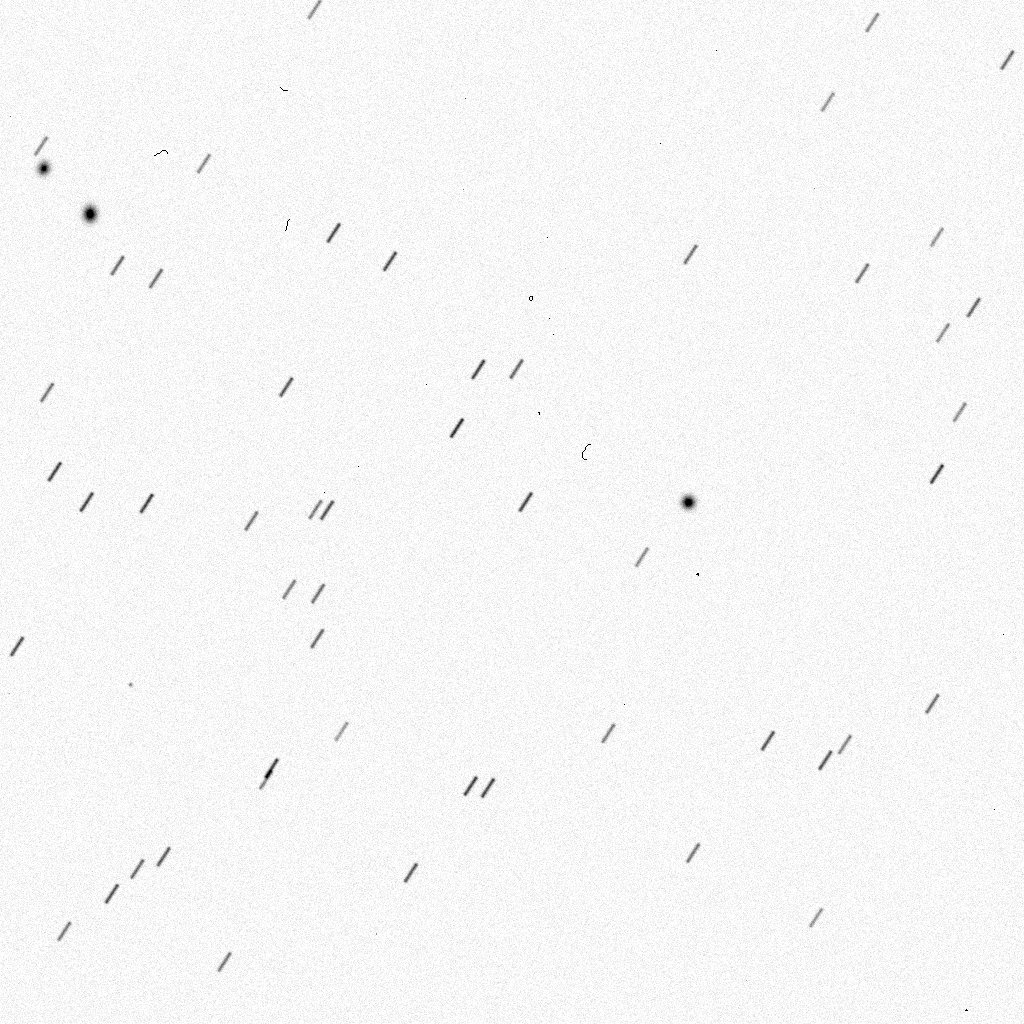
\includegraphics[width=\textwidth]{images/fullframestargen1.jpg}
    \end{subfigure}
    \begin{subfigure}[t]{.4\textwidth}
        \centering
        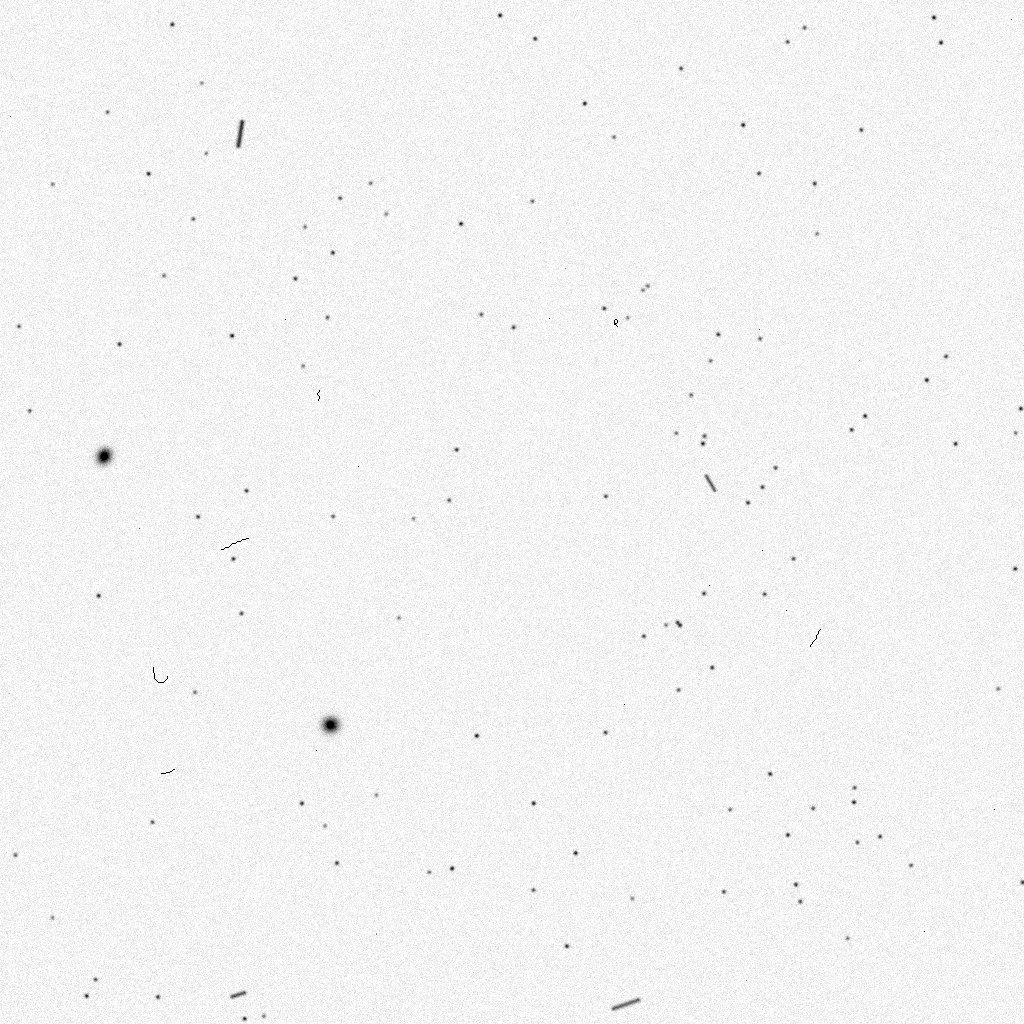
\includegraphics[width=\textwidth]{images/fullframestargen2.jpg}
    \end{subfigure}

    \caption{Synthetic images with a resolution of 1024x1024 generated by starGen.}
    \label{fig:stargenfullframe}
\end{figure}


However, when training the network, we need a 50x50 image with only one object present. To achieve this, we can generate full-frame images and cut out a 50x50 window with one object or we can use starGen to generate images of a given size with just one object. As it was easier to configure the parameters of each object we have decided to generate 50x50 images with one object and produce the training and validation set of data for the network.

Images were generated in 4 iterations, where each iteration represented a degree of brightness of objects. We have generated the following iterations:
\begin{enumerate}
    \item Objects with high brightness (HB)
    \item Objects with medium brightness (MB)
    \item Objects with low brightness (LB)
    \item Objects with very low brightness (VLB)
\end{enumerate}

In the Table \ref{table:bright} we show the brightness range of objects for each iteration. The iteration contains a training and validation set, with objects of the defined brightness. Each iteration could be used independently to train the network. However in our case, after generating all iterations we have merged them together to create the dataset that contains various brightness of objects. 

{\renewcommand{\arraystretch}{1.2}
\begin{table}[h]
\centering
    \begin{tabular}{|l|l|l|}
    \hline
     & \textbf{point, streak, cut streak, galaxy} & \textbf{hot pixels, cosmic rays} \\ \hline
    \textbf{HB}     & <40 000, 60 000>  & <60 000, 65 535> \\ \hline
    \textbf{MB}     & <10 000, 40 000>  & <50 000, 60 000> \\ \hline
    \textbf{LB}     & <2 000, 10 000>   & <10 000, 50 000> \\ \hline
    \textbf{VLB}    & <500, 2 000>      & <2 000, 10 000>  \\ \hline
    \end{tabular}
\caption{Brightness range of generated objects for each iteration.}
\label{table:bright}
\end{table}}


Generating data for the training set, we aimed to have a robust dataset that covers all possible scenarios. For this reason images for the streak, cut streak, and galaxy classes were generated using the Cartesian product of some parameters rather than just choosing randomly from an interval. With streaks, for each $length$ of the streak and each rotation $alpha$, we have generated one image with randomly selected $brightness$ and $fwhm$ from the interval. For both $length$ and $alpha$ the numbers from the interval were selected using an increment of 1. 
%For the length we have selected numbers ranging from 1 to 10 and rotation alpha from 0 to 180 degrees. This gave us a total of 1800 images. 
The same process was followed for cut streaks. 
With galaxies, the Cartesian product of standard deviations $sigmaX$ and $sigmaY$ was used. And for each $sigmaX$ and $sigmaY$ two images were generated, where the other parameters like $alpha$, $brightness$, $brightnessFactor$ and $sigmaFactor$ were selected randomly from the interval. Both standard deviations were selected from the interval with an increment of 0.1. 
%The selected standard deviations were numbers from 1.5 to 4.5 with an increment of 0.1. 
Points, hot pixels, and cosmic rays don't have a lot of parameters to configure, therefore values of parameters were chosen randomly from the interval. However with cosmic rays, for each type, we have generated the same amount of images to keep the dataset balanced. 

Data for the validation set were generated by randomly choosing the value of the parameters from the interval. To preserve the balance of the dataset, each object has the same amount of generated images.

Parameters for each object that were used during the generation of images are depicted in the Table \ref{table:params}. The parameter $brightness$ is not shown in the table since it depends on the data iteration, while the other parameters in the table stay fixed for each iteration. These parameters apply to both the training and validation set. 

{\renewcommand{\arraystretch}{1.2}
\begin{table}[h]
\centering
    \begin{tabular}{|l|l|}
    \hline
    \textbf{Object} & \textbf{Parameters} \\ \hline
    \textit{point} & fwhm = <3.5, 4> \\ \hline
    \textit{streak, cut streak} & \begin{tabular}[c]{@{}l@{}}fwhm = <3.5, 4>\\ length = <1, 10>\\ alpha = <0, 180>\end{tabular} \\ \hline
    \textit{galaxy} & \begin{tabular}[c]{@{}l@{}}alpha = <0, 180>\\ sigmaX = <1.5, 4.5>\\ sigmaY = <1.5, 4.5>\\ brightnessFactor = <0.6, 0.8>\\ sigmaFactor = <0.2, 0.4>\end{tabular} \\ \hline
    \textit{hot pixels} &  \\ \hline
    \textit{cosmic rays} & \begin{tabular}[c]{@{}l@{}}pixelCount = <5, 30>\\ spotPixelCount = <2, 15>\end{tabular} \\ \hline
    \end{tabular}
\caption{Parameter intervals used for the generation of objects.}
\label{table:params}
\end{table}}


To make the generated data look realistic we added various noises. Gaussian noise was applied to each image with $std$ of 100 and $mean$ 200. We also applied Poisson noise to each object. And finally, we used both real DARK and FLAT FIELD frames on our images. Note, that we didn't use the BIAS frame, since the DARK frame we are using already contains the BIAS frame. We have obtained these master frames with a resolution of 1024x1024 pixels, and used the $windowCutter.py$ script to cut 50x50 images. We mentioned in Section \ref{sec:photoreduction} that the DARK frame changes significantly with different exposure times. To account for this, we are using four DARK frames with exposure times of 5, 60, 90, and 360 seconds. For each of these frames, the above-mentioned process of generating objects was used and therefore increasing the amount of data four times, for both training and validation sets.

To sum up, the generated training set for one iteration contains 1800 images for each class, multiplied by 4 DARK frames giving a total of 7200 images per class. After adding all iterations together, the training set consists of 28 800 images per class and a total of 172 800 images. 

For one iteration of the validation set, 1000 images per class were generated. Multiplying by 4 DARK frames gives a total of 4000 images per class. Merging iterations together results in 16 000 images per class for a total of 96 000 images.

% \chapter{Research} \label{chap:research}

\section{Kubernetes security automation}
\label{sec:kubernetes-security-automation}

This section introduces the reader to the topic of the security automation inside the Kubernetes cluster. We discuss different security tools, their place in the cloud Infrastructure and examine their usage patterns. Additionally, we explain why were the specific tools chosen for our research.

\subsection{Overview}

Kubernetes security scanners and operators provide an array of defensive capabilties. Most of them act in the form of informator. That is, they do not perform any remediatory actions, but only provide user with information about the cluster security status. Nevertheless, there are some solutions on the market that are capable of resolving some of the security issues automatically. This, on the other hand, introduces another layer of concern: can we really trust a third-party system to introduce modifications to our infrastructure? That the former type is the most abundant and is the focus of this paper. Automatic remediation can be then implemented as a part of CI/CD pipeline based on the scan results. This ensures that it is compliant with the company's policies and is tailored to the company's needs.

One of the ways to classify Kubernetes security scanners is by the scan target. Here we can roughly divide them into three groups: configuration file scanners, cluster scanners and container image scanners. Most of the tools, however, can be put into multiple different groups. Cluster scanners usually are able to perform container image scanning as well and it is a part of the full cluster scan. Cluster scanners detect misconfigurations in the cluster infrastructure and its essential components. They look for, among other things, containers running with extensive privilages, exposed sensitive workloads and plaintext secrets. Container image scanners look for known vulnerabilities inside the images. Configuration file scanners perform a scan of the cluster configuration files. For large infrastructure with a number of applications deployed there might be over several tens of thousands lines of configuration and such scanners aim to detect any known misconfigurations by going through theese lines.

Cluster security scanners can be further classified by the execution point. Again, there is usually more than one way to run a scan, but here are a few options: run a scanner tool as a container, run it from a remote machine connected to the cluster, run it is an operator, which can perform scan automatically on a regular basis. To always keep cluster up-to-date with the most recent security patches the best solution would be to either install an operator or integrate a security scanner tool into your CI/CD pipeline.

\subsection{Selection Criteria}

To perform our assessment we have chosen from a variety of Kubernetes security scanners. Though the area is still relatively new, there is a variety of tools with different purposes available on the market. We made our choice based on the following criteria:
\begin{itemize}
\item \textbf{free-to-use} \\
We do include some proprietary tool testing further in our research as an additional comparison, however, for the main part we only use free tools. Kubernetes itself is distributed under Apache License 2.0, which means it is inherently free to use. The ability to adopt these tools without financial constraints enables wider adoption, thus, contributing to the community-driven innovations. Finally, this research not being funded, we could only afford to work with openly distributed software.
\item \textbf{open-source} \\
Again, we are sticking to the open-source nature of the Kubernetes. By selecting open-source tools, this research ensures that each tool's codebase is transparent and can be reviewed by security experts. This transparency increases trust in the tools' effectiveness, as the community can spot, disclose, and even patch any vulnerabilities in the software. Another advantage is the customization of the open-source software as the companies can adapt the tools to their specific Kubernetes security needs.
\item \textbf{designed with cloud in mind} \\
Designed to be used in the Kubernetes environment specifically, these tools should offer features like scanning container images for vulnerabilities, but also monitoring network policies, securing Kubernetes configuration files, or identifying misconfigurations within clusters. Tools built specifically for Kubernetes are more efficient, as they are optimized to address the distinct aspects of the platform, making security management more effective.
\item \textbf{has an active community support} \\
Tools with active communities tend to have more frequent updates, faster response times for bug fixes, and a wide range of contributors who bring diverse insights to improve functionality and security. The world of the software security is changing rapidly and an active community means that the tool is up-to-date with the most recent events. A thriving community also means that users can easily access support on the community forums.
\end{itemize}

Based on the aforementioned criteria we ended up choosing and testing the following tools:
\begin{itemize}[noitemsep]
\item Trivy
\item Kube-bench
\item Prowler
\item Kubescape
\end{itemize}

In the next chapters we closely examine each selected tool and explain how it is matches our selection criteria. Additionally, we compare them to each other and highlight their strong and weak sides.

\subsection{Trivy}
Trivy is an Aqua Security open source project with a vast array of use cases. It supports multiple scan targets and includes multiple scanners. Among the supported targets are:
\begin{itemize}[noitemsep]
    \item Container Image
    \item Filesystem
    \item Git Repository 
    \item Virtual Machine Image
    \item Kubernetes
\end{itemize}
Trivy includes scanners for:
\begin{itemize}[noitemsep]
    \item OS packages and software dependencies in use (SBOM)
    \item Known vulnerabilities (CVEs)
    \item IaC issues and misconfigurations
    \item Sensitive information and secrets
    \item Software licenses
\end{itemize}

According to the Trivy official Gihub page \cite{trivy-github}, it can be installed on the local machine using any of the popular package mangager or by downloading a binary from the Github Releases. It can also be ran as a Docker container or Kubernetes Operator. Furthermore, Trivy can be integrated into GitHub Actions or installed as a Visual Studio Code plugin. Aqua Security uploads each new release as a Docker image into the Dockerhub repository. There is a variety of supported configuration parameters for Trivy Kubernetes scanning feature. Users can specify which scanners to include, which namespaces to skip, which nodes to scan and the format of the output. An example of a Trivy misconfiguration scan command executed against the default Kubernetes context, which would output a short summary of findings and skip \textbf{dev-system} namespace, is included below (see Listing~\ref{lst:trivy-k8s}).

\begin{center}
    \begin{lstlisting}[language=bash, caption={[An example of a Trivy Kubernetes scan command] An example of a Trivy Kubernetes scan command.}, label={lst:trivy-k8s}]
    $ trivy k8s \
        --scanners=misconfig \
        --report=summary \
        --exclude-namespace=dev-system
    \end{lstlisting}
\end{center}

Since Kubernetes is listed as a natively supported target and Trivy can scan for both vulnerabilities and misconfigurations, Trivy is well-suited for our research. It is also open source and available for free. Presently, Trivy's Github repository has over 2800 issues, with a little over than 150 of them being open, repository's commit history shows active development with a bi-monthly minor release cycle and yearly major release cycle. Thus, we can assume an active community and developer support.

\subsection{Kube-bench}
Kube-bench is another open source tool developed by Aqua Security. Their Github page \cite{kube-bench-github} states that it checks whether Kubernetes is deployed securely by running the checks against the CIS Kubernetes Benchmark (see \ref{sss:cis-kubernetes-benchmark}). Kube-bench is designed specifically for Kubernetes. Users can run the it inside a Docker container or deploy it as a Kubernetes job, however, there is still an option to download the binary on the local machine and run it against the desired Kubernetes cluster.

Since kube-bench has a much narrower feature set than Trivy, it is much more simple in usage, but still highly configurable. Configuration can be supplied via a config file or we can pass the configuration parameters directly using one of the 24 flags. An example of a simple scan command targeting \textbf{master}, \textbf{node}, \textbf{etcd}, \textbf{policies} CIS Benchmark categories is provided in Listing~\ref{lst:kube-bench-scan}.

\begin{center}
    \begin{lstlisting}[language=bash, caption={[An example of a Kube-bench scan command] An example of a Kube-bench scan command.}, label={lst:kube-bench-scan}]
    $ kube-bench run \
        --targets master,node,etcd,policies
    \end{lstlisting}
\end{center}

Kube-bench is actively supported by the developers and the community. At the present moment, Kube-bench Github repository has about 500 issues, 10\% of which are currently open. Repository receives updates on a weekly basis and the new version is released monthly.

\subsection{Prowler}

Prowler, as described on the Github page \cite{prowler-github}, is an open source security tool designed to perform Kubernetes security best practices assessments, audits, incident response, continuous monitoring, hardening and forensics readiness, and remediation. It is shipped with a built-in dashboard, which displays scan results in graphical format (see Fig~\ref{img:prowler-dashboard}). However, the dashboard can only read the scan results from the folder on the host machine and the user cannot trigger a new scan directly from the dashboard. Users have to install a separate Prowler App inside the clusters to trigger the scan. According to the documentation \cite{prowler-app-page}, ``it provides a user-friendly interface to configure and run scans, view results, and manage your security findings.''

\begin{figure}[!hbt]
	\begin{center}
		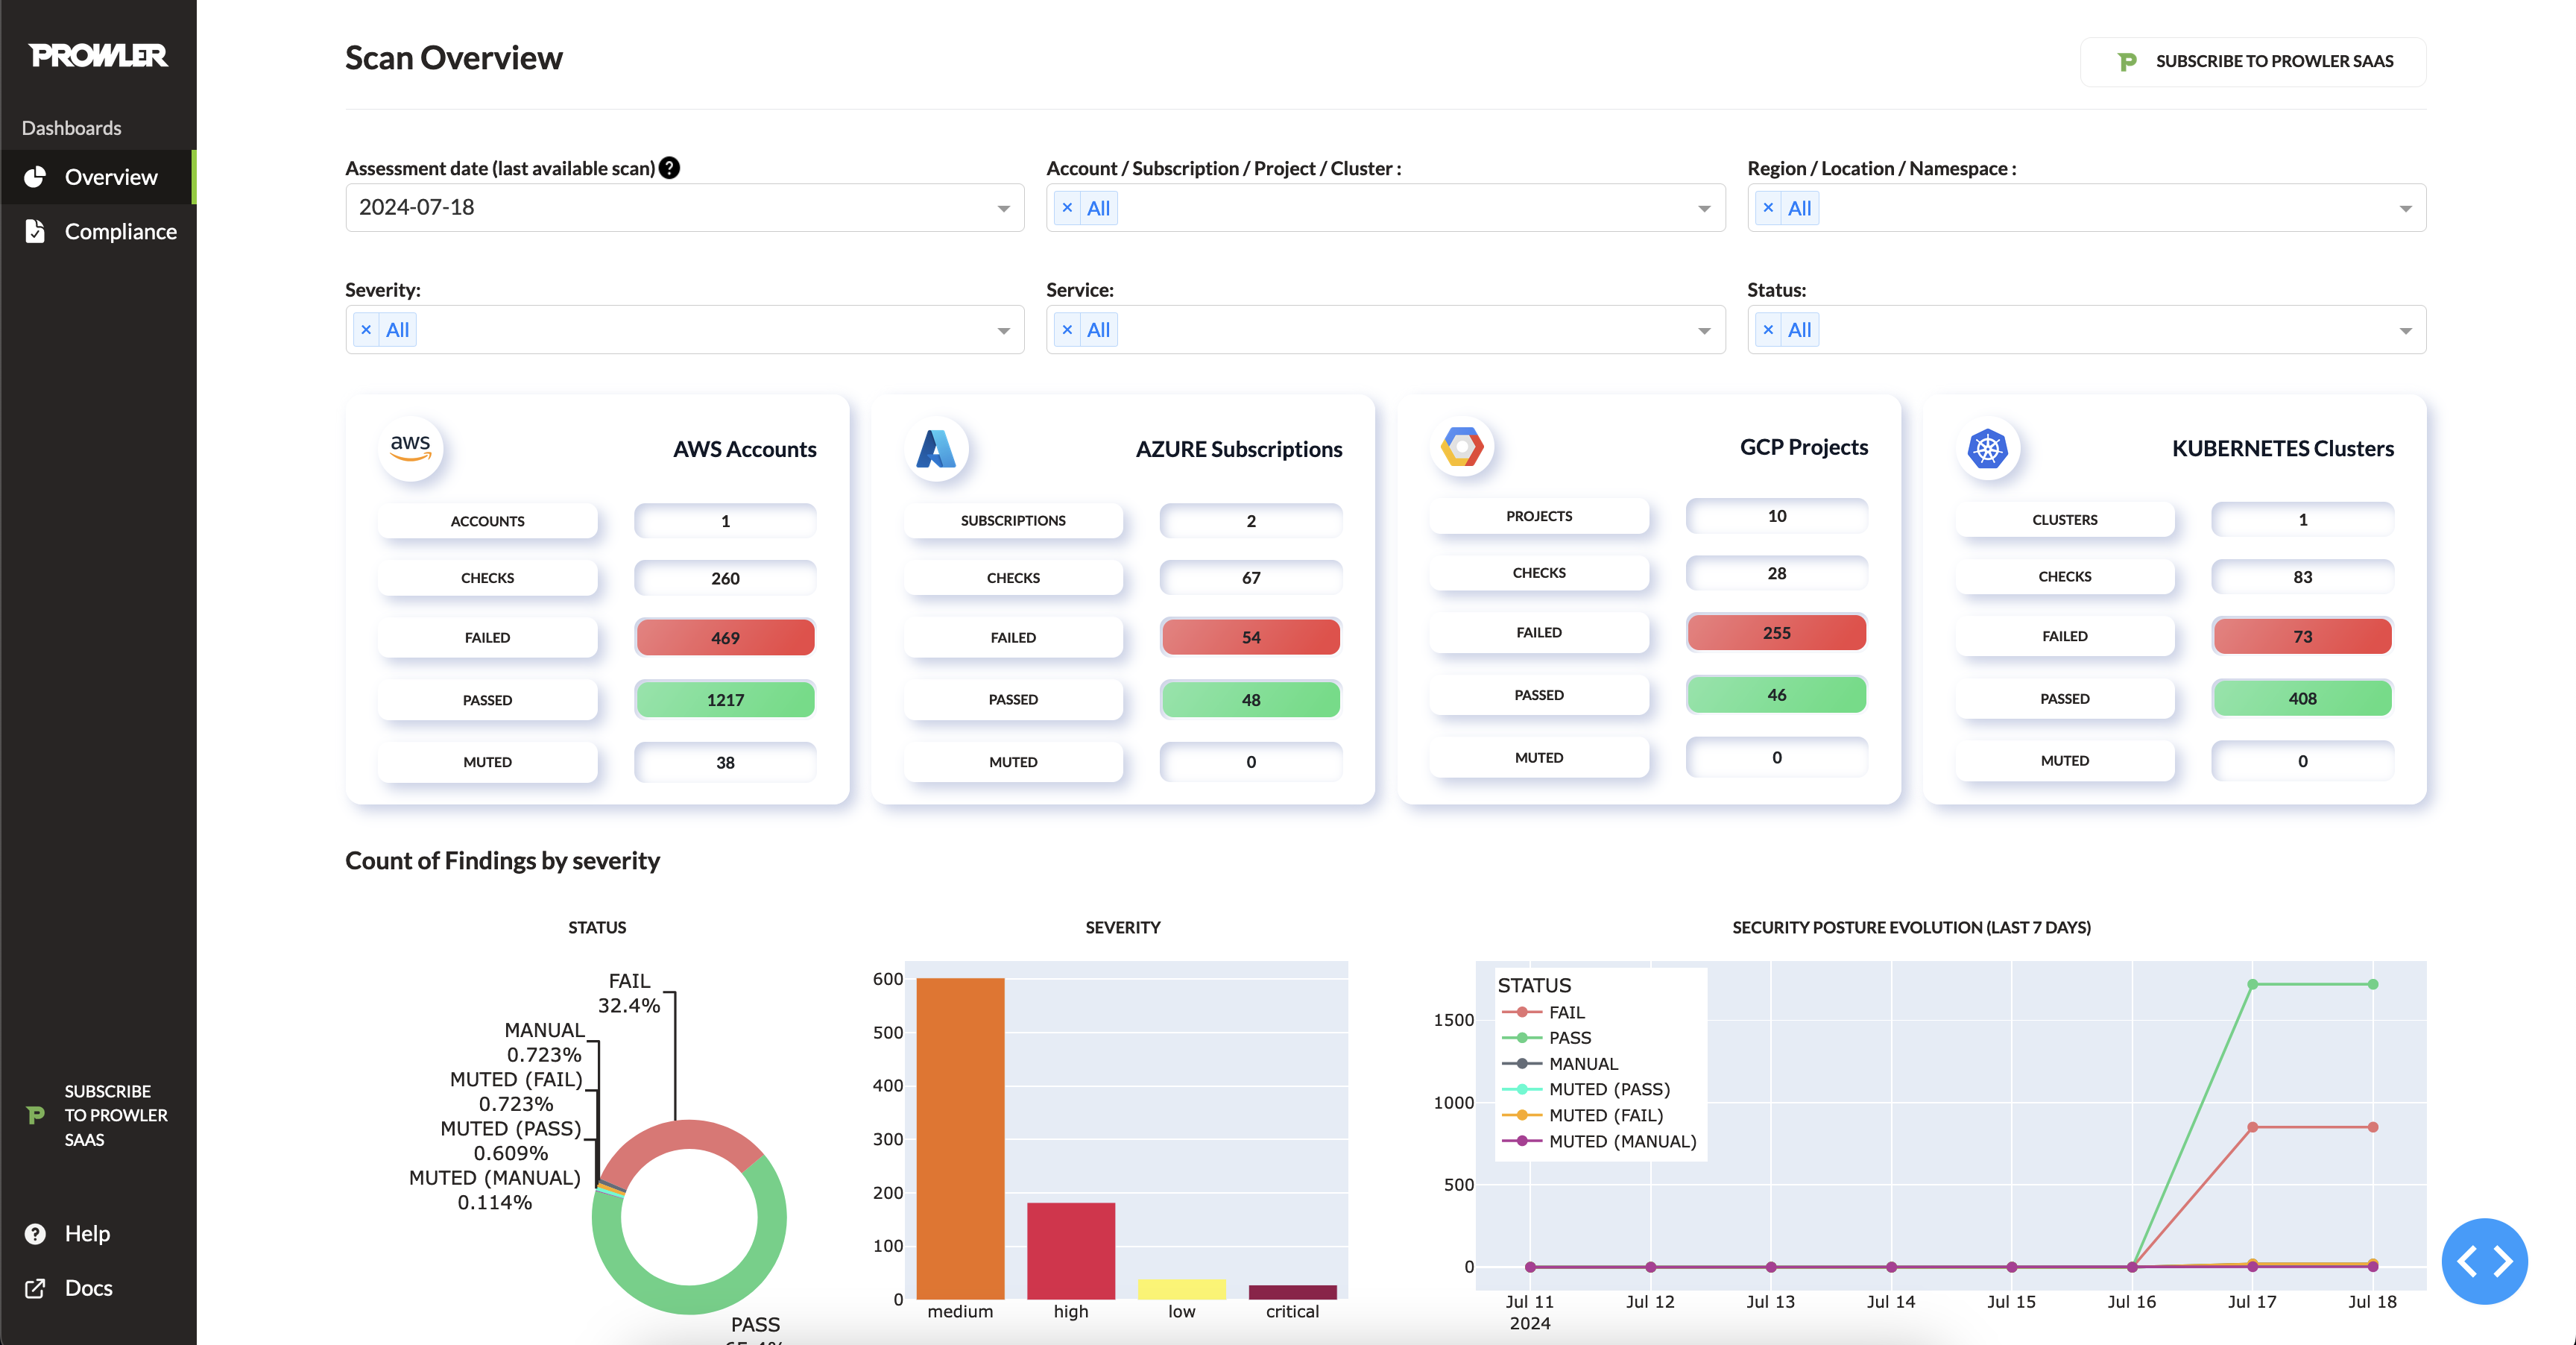
\includegraphics[width=0.85\textwidth]{images/prowler-dashboard.png}
        \caption{Prowler dashboard interface.}
		\label{img:prowler-dashboard}
	\end{center}
\end{figure}

Prowler CLI supports Azure, Google Cloud, AWS and generic Kubernetes providers. It performs a scan against multiple Kubernetes security frameworks to ensure the best coverage. Prowler supports output in CSV or JSON-OCSF format, the latter being an independent open source developed JSON schema by Open Cybersecurity Schema Framework project, which has recently joined the Linux Foundation organization. Again, we configure the Prowler job either via a configuration file or by passing the flags directly in the execution command. Listing~\ref{lst:prowler-command} provides an example on how can a Prowler scan be triggered. This particular execution would output the results in \textbf{json-ocsf} format, including only failed and manual checks.

\begin{center}
    \begin{lstlisting}[language=bash, caption={[An example of a Prowler scan command] An example of a Prowler scan command.}, label={lst:prowler-command}]
    $ prowler kubernetes \ 
        --status FAIL,MANUAL \
        --output-formats json-ocsf
    \end{lstlisting}
\end{center}

There are over a thousand issues in official Prowler Github repository. The development is still in progress and the tool receives regular updates. The project has an active community with operational development support.

\subsection{Kubescape}
Kubescape is an open-source security platform designed to harden the security of a Kubernetes cluster. Kubescape CLI allows users to scan the cluster from the local machine. Kubescape Operator enables image vulnerability scanning as well as continuous and scheduled scanning. Kubescape also offers Github Actions integration for CI/CD pipelines according to the official Github page \cite{kubescape-github}.

Kubernetes cluster is verified against a posture library (available at Github \cite{regolibrary-github}), which is a collection of frameworks each containing a set of controls. By default, the library is comprised of NSA Framework controls, MITRE ATT\&CK Framework controls and CIS Benchmark controls.

Scan configuration is again passed with multiple flags. There are flags allowing to select the namespaces to include into scan, namespaces to exclude from the scan, output format and location. Scanning can be then performed using the command displayed in Listing~\ref{lst:kubescape-command}.

\begin{lstlisting}[language=bash, caption={[An example of a Kube-bench scan command] An example of a Kube-bench scan command.}, label={lst:kubescape-command}]
    $ kubescape scan \
        --format json \
        --output kubescape-scan.json
\end{lstlisting}

Unfortunately, when executed in this mode, Kubescape performs only a few checks. In order to perform complete vulnerability and misconfiguration scan, Kubescape requires Kubescape Operator installed in the cluster. 

Kubescape's repository shows ongoing development with regular update releases.

\subsection{Preliminary Comparison}

This section compares the selected tools based on their declared feature set, ease of installation and execution, scan targets, supported cloud providers and security frameworks. This comparison does not include the analysis of the scan results, performance or any other aspects of execution. A detailed analysis of the generated reports can be found in Chapter~\ref{chap:results}.

We start by comparing the scanners by their feature set. Trivy has the most broad feature set as it is able to scan for vulnerabilities inside the images, perform IaC scan (supporting Terraform, Helm, plain Kubernetes YAML), scan for misconfigurations in Kubernetes resources and generate SBOM. Kube-bench is designed to perform only two tasks: CIS Kubernetes Benchmark checks and Node-level audit, making it very specialized tool. Prowler is able to detect misconfigurations and security threats, perform CIS Benchmark checks and cloud security audit. Kubescape's features include misconfiguration and container vulnerability scanning, RBAC risk analysis and SBOM generation. While all of the scanners can detect Kubernetes misconfigurations, only Trivy and Kubescape have the ability to scan for the vulnerabilities in containers. SBOM generation is a requirement for enterprise-level scanners nowadays, which makes Kubescape and Trivy stand out once again.

When we compare the tools by the supported cloud providers, simplicity of Kube-bench makes it the leader in this category. Since Kube-bench only performs static analysis, this makes it cloud agnostic, meaning that it can be used with any cloud provider as long as the provider offers Kubernetes services. Trivy, Kubescape and Prowler all support the same cloud providers. Kubescape and Trivy both natively support AWS, Azure and GCP. Prowler's focus is AWS, but it also supports Azure and Google Cloud Platform.

All of the presented tools declare full CIS Benchmark coverage, which is the only supported framework for Kube-bench. Trivy additionally declares NSA and MITRE ATT\&CK coverage. Kubescape further extends the set with NIST 800-53 and SOC 2 frameworks, which are more specialized frameworks, the former developed by the U.S. government and focuses on technical and administrative controls, while the latter focuses on the customer data security and compliance. Prowler mixes the CIS Benchmark checks with the four major security and privacy frameworks or regulations relevant to organizations handling sensitive data (PCI-DSS, GDPR, HIPAA, ISO27001).

From the user perspective we can compare the scanners by the ease of installation and execution. Trivy's binary is available for download using most of the popular package managers (like Brew for MacOS and apt-get, yum, pacman and others for various Linux distros). Less secure but more convenient way of installation is by using a script. Additionally, Trivy has a Docker image available in Docker Hub, GitHub Container Registry and AWS Elastic Container Registry. Trivy can be executed against an active Kubernetes context using the binary or installed as an operator inside the cluster for automatic scanning every six hours. Kube-bench can only be run from inside the container. Kube-bench provides a \textbf{job.yaml} file, which can be used to run it inside the cluster as a Kubernetes Job. Kube-bench runs checks specified in controls files that are a YAML representation of the CIS Kubernetes Benchmark checks. Kubescape supports the usual installation channels. Additionally, users are able to download scan artifacts (frameworks) separately. Kubescape Operator can be installed inside the using a Helm chart. Unfortunately, Kubescape Operator must be installed in the cluster for the Kubescape CLI to be able to scan for vulnerabilities. Prowler CLI can be installed only as a Python module, but there are also Docker images available to download from the Docker Hub and AWS Public ECR. Prowler also provides an applciation, which displays scan results in a graphical format. Table~\ref{tab:preliminary-scanner-comparison} summarizes our preliminary comparison findings.

\begin{table}[H]
    \begin{center}
        \begin{tabular}{
            | >{\raggedright\arraybackslash}p{.15\textwidth} 
            | >{\raggedright\arraybackslash}p{.22\textwidth} 
            | >{\raggedright\arraybackslash}p{.15\textwidth} 
            | >{\raggedright\arraybackslash}p{.20\textwidth} 
            | >{\raggedright\arraybackslash}p{.15\textwidth} | }
        \hline
        \textbf{Tool} & \textbf{Features} & \textbf{Cloud support} & \textbf{Frameworks} & \textbf{User experience} \\
        \hline\hline
        Trivy & Vulnerability scan, Misconfiguration scan, IaC scan, SBOM generation, Operator & AWS, Azure, GCP & CIS, NSA, MITRE ATT\&CK & CLI tool \\
        \hline
        Kube-bench & CIS Benchmark audit & cloud agnostic & CIS & Kubernetes Job \\
        \hline
        Prowler & Cloud audit, misconfiguration scan, compliance scan, Operator & AWS, Azure, GCP & CIS, PCI-DSS, GDPR, HIPAA & CLI tool, UI app \\
        \hline
        Kubescape & Operator, misconfiguration scan, vulnerability scan, SBOM generation, RBAC analysis & AWS, Azure, GCP & CIS, NSA, MITRE ATT\&CK, NIST 800-53, SOC 2 & CLI tool \\
        \hline
        \end{tabular}
    \end{center}
    \caption{Kubernetes security scanners preliminary comparison.}
    \label{tab:preliminary-scanner-comparison}
\end{table}
\section{Security Threats Classification}
\label{sec:security-threats-classification}

We propose the following classification of the potential Kubernetes security risks. This is largely based on the security best practices gathered by Aquasec \cite{aquasec-security-best-practices,aquasec-kubernetes-vulnerability-database-misconfigurations}. We group related security threats into common subcategories and convert everything into the table format making it easier to navigate and study.

\begin{table}[H]
    \begin{center}
        \begin{tabular}{ | p{.27\textwidth} | p{.27\textwidth} | p{.40\textwidth} | } 
        \hline
        Category & Subcategory & Description \\ [0.5ex] 
        \hline\hline
        \multirow{5}{*}{} 1. Configuration Vulnerabilities & 1.1 Misconfigured RBAC  & Incorrectly set roles and permissions can lead to unauthorized access.  \\ \cline{2-3} 
                & 1.2 Pod Security Policies & Weak or missing pod security policies can allow privileged containers or insecure configurations.  \\ \cline{2-3} 
                & 1.3 Network Policies  & Inadequate network policies can expose services to unauthorized access.  \\ \cline{2-3} 
                & 1.4 Resource Limits  & Absence of resource limits (CPU, memory) can lead to resource exhaustion.  \\ \cline{2-3} 
                & 1.5 Preemption Policies & Undefined preemption policies/priorities. \\ \hline
        \multirow{3}{*}{} 2. Container Vulnerabilities & 2.1 Base Image Vulnerabilities &  Using container base images with known vulnerabilities. \\ \cline{2-3} 
                & 2.2 Outdated Packages & Containers running outdated software with known exploits. \\ \cline{2-3} 
                & 2.3 Exposed Secrets & Sensitive data (tokens, passwords) exposed in environment variables or volumes. \\ \hline
        \multirow{3}{*}{} 3. Kubernetes API Server Vulnerabilities & 3.1 API Server Exposure &  Unrestricted access to the Kubernetes API server. \\ \cline{2-3} 
                & 3.2 Audit Logging & Lack of or improperly configured audit logging that hinders incident detection and response. \\ \cline{2-3} 
                & 3.3 ETCD Data Exposure & Unsecured etcd exposing sensitive cluster data. \\ \hline
        \multirow{2}{*}{} 4. Network and Communication Vulnerabilities & 4.1 Service Exposure &  Services unnecessarily exposed to the internet. \\ \cline{2-3} 
                & 3.2 Ingress/Egress Controls & Inadequate controls over ingress and egress traffic. \\ \hline
        \multirow{2}{*}{} 5. Runtime and Execution Vulnerabilities & 5.1 Runtime Privileges &  Containers with root or elevated privileges. \\ \cline{2-3} 
                & 5.2 Containers with root or elevated privileges. & Usage of insecure system calls from within containers. \\ \hline
        \end{tabular}
    \end{center}
    \caption{Kubernetes security threat classification.}
    \label{tab:kubernetes-security-threat-classification}
\end{table}
\section{Experimental Environment}
\label{sec:experimental-environment}



% \chapter{Results} \label{chap:results}

In this chapter, we will test the selected models on the testing dataset, which contains 300 real images acquired by AGO70. First, we will test the model trained on the synthetic data from the Section \ref{subsec:finalmodel}. Next, we will test the models that were fine-tuned using real data in the training process. We proposed two approaches and have therefore two different models (Sections \ref{subsec:mergedmodel}, \ref{subsec:fcmodel}), which will be both tested separately. Finally, we will compare the performance of our models to the pre-trained ResNet-18 model. 

To measure the performance of our model we are using the following metrics: 
\begin{equation}
    Accuracy = \frac{TP + TN}{TP + FP + TN + FN}
\end{equation} 
\begin{equation}
    Recall = \frac{TP}{TP + FN}
\end{equation}
\begin{equation}
    Precision = \frac{TP}{TP + FP}
\end{equation}
where TP are true positives, FP are false positives, TN are true negatives and FN are false negatives. 

\section{Model trained on the synthetic data}

The final model from Section \ref{subsec:finalmodel} was evaluated on the testing dataset and has achieved 73.00 \% accuracy, 73.52 \% precision and 73.00 \% recall. 

From the confusion matrix in the Figure \ref{img:confmatrixsyn} we can see that the model has the biggest problem distinguishing between galaxy and streak (more than 30 cases). This is caused by the fact that elliptical galaxies with a high degree of ellipticity resemble streaks and even professionals wouldn't be able to tell the difference just from one image. Another prevalent problem is the misclassification of streaks as points (10 cases) and points as cosmic rays (13 cases). In the Figure \ref{fig:wrongsyn} we show some examples of wrongly classified images, where we can see that these problems are usually caused by small streaks that resembled points (\ref{fig:streakpointmis3}), and points with small fwhm which caused them to look like spots (\ref{fig:pointcosmicmis3}).   

\begin{figure}[h]
    \centering
    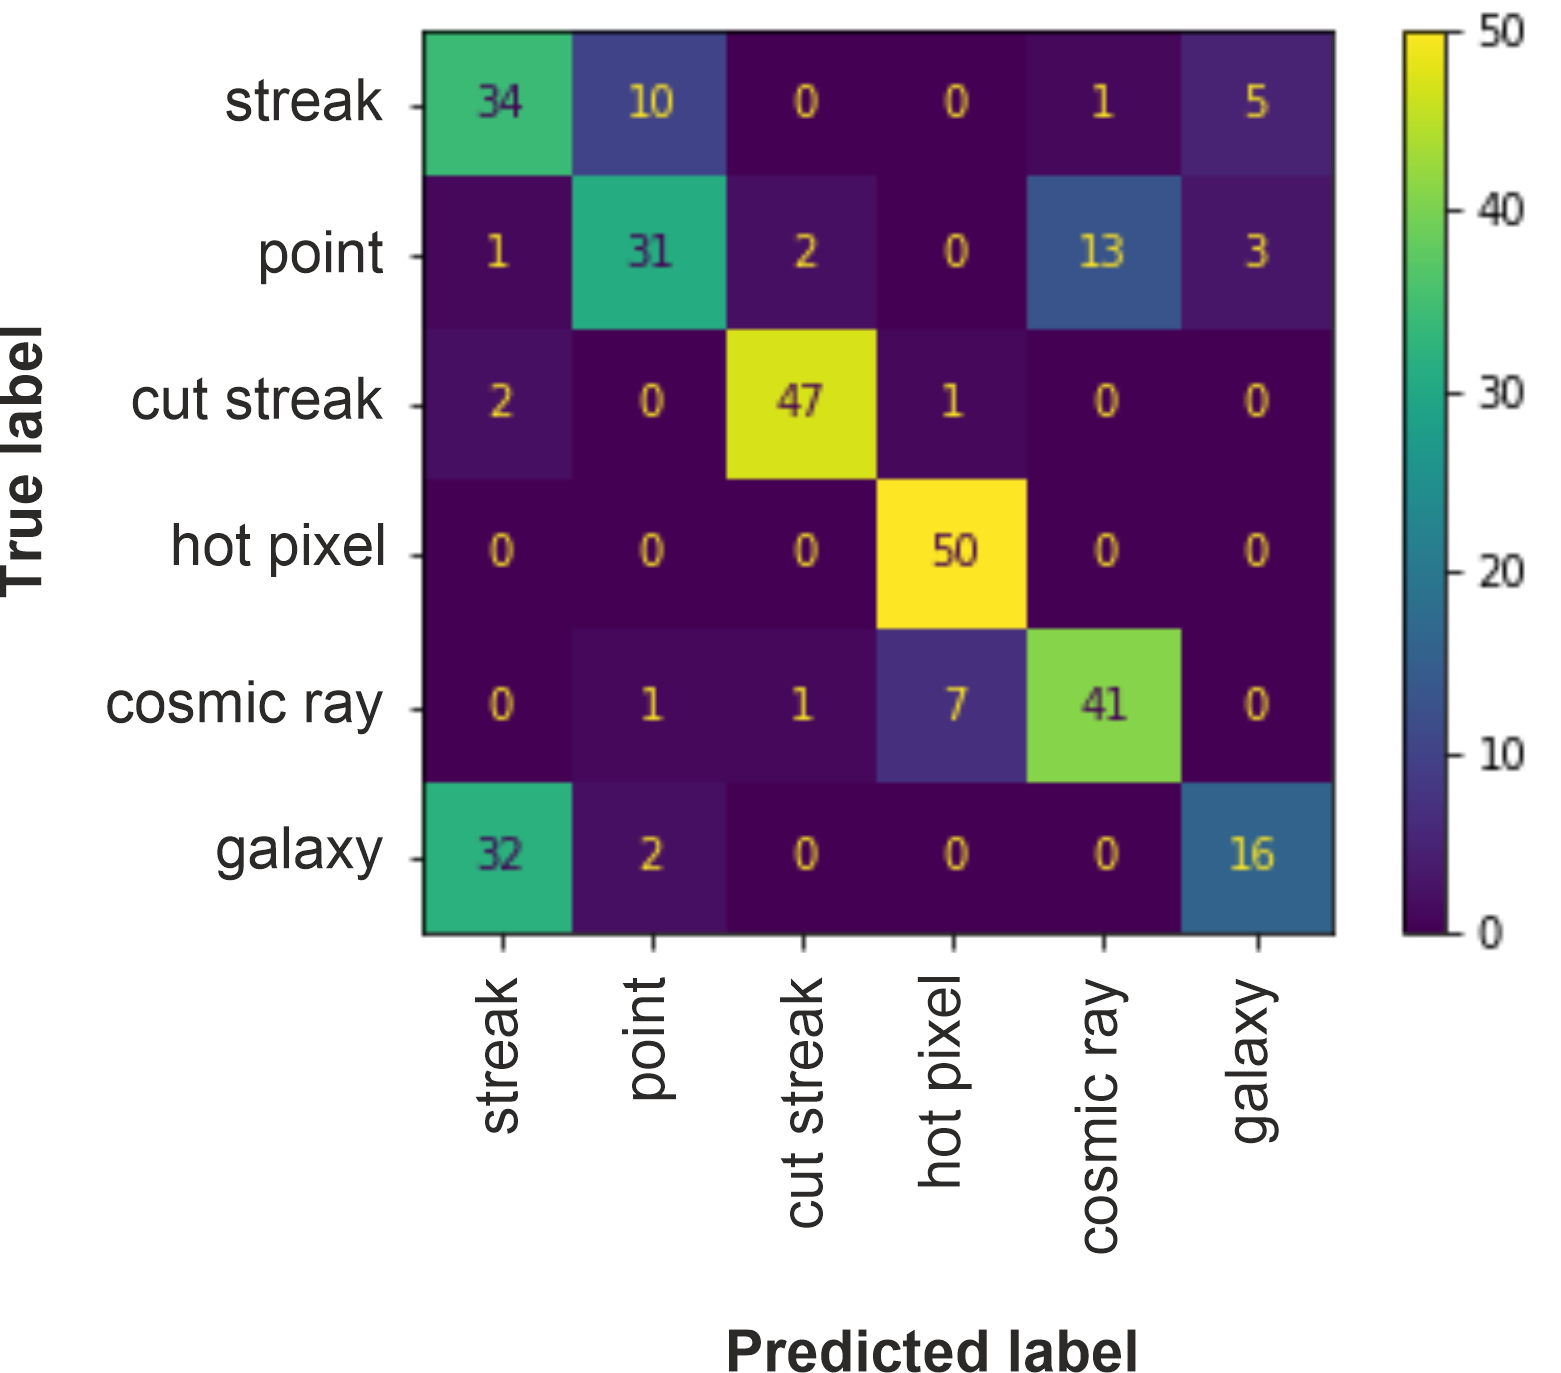
\includegraphics[width=.5\textwidth]{images/confusionmatrix51.png}
    \caption{Confusion matrix from the testing of the final model trained only on synthetic data.}
    \label{img:confmatrixsyn}
\end{figure}

\begin{figure}[!h]
\centering
    \begin{subfigure}[t]{.23\textwidth}
        \centering
        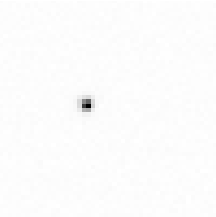
\includegraphics[width=\textwidth]{images/wrongImage8.png}
        \caption{}
        \label{fig:pointcosmicmis3}
    \end{subfigure}
    \begin{subfigure}[t]{.23\textwidth}
        \centering
        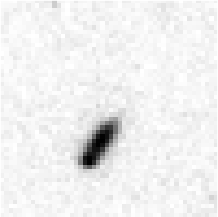
\includegraphics[width=\textwidth]{images/wrongImage18.png}
        \caption{}
    \end{subfigure}
    \begin{subfigure}[t]{.23\textwidth}
        \centering
        
\includegraphics[width=\textwidth]{images/wrongImage34.png}
        \caption{}
    \end{subfigure}
    \begin{subfigure}[t]{.23\textwidth}
        \centering
        \includegraphics[width=\textwidth]{images/wrongImage48.png}
        \caption{}
        \label{fig:streakpointmis3}
    \end{subfigure}

    \caption[Wrongly classified images on the model that trained only with synthetic data.]{Wrongly classified images on the model that trained only with synthetic data. (a) A point misclassified as a cosmic ray, (b) A galaxy misclassified as a streak, (c) A streak misclassified as a galaxy, (d) A streak misclassified as a point. }
    \label{fig:wrongsyn}
\end{figure}



\section{Model trained on the merged data}
% obidva modeli ze dame testovat
% tabulka s vysledkami na provonanie
% vyjadrenie ze ktory je lepsi
% ukazat matice a acc, recall ... 
% tuto asi bude dobre spravit subsubsection a tam kazdy model opisat
% a potom spravit dalsiu kde ich porovnam nejak

% este to porovnat aj s resnetom nejak

On the testing dataset, the model from Section \ref{subsec:mergedmodel} has achieved an accuracy of 87.00 \%, precision of 87.15 \% and recall of 87.00 \%. Of 300 images only 39 were wrongly classified. 

From the confusion matrix in the Figure \ref{img:confmatrixmerged} we can see that the model has classified 14 cases of galaxies as streaks. This could be caused again by the fact that several samples of galaxies have a sharp elliptical shape that resembles a streak (\ref{fig:galaxystreakmis2}). 
Apart from this only a small amount of misclassified images is with streak and galaxy (5 cases), streak and point (4 cases) and cosmic rays and hot pixels (4 cases). Some cases of the wrongly classified images are depicted in the Figure \ref{fig:wrongmerged}. We can see that a cosmic ray which has very few pixels have been classified as a hot pixel (\ref{fig:cosmichotpixelmis}), or a very short streak was predicted as a point (\ref{fig:streakpointmis2}). 

\begin{figure}[h]
    \centering
    \includegraphics[width=.5\textwidth]{images/confusionMatrix13r_0.png}
    \caption{Confusion matrix from the testing of the model trained on merged synthetic and real data.}
    \label{img:confmatrixmerged}
\end{figure}

\begin{figure}[!h]
\centering
    \begin{subfigure}[t]{.23\textwidth}
        \centering
        \includegraphics[width=\textwidth]{images/mwrongImage10.png}
        \caption{}
        \label{fig:galaxystreakmis2}
    \end{subfigure}
    \begin{subfigure}[t]{.23\textwidth}
        \centering
        \includegraphics[width=\textwidth]{images/mwrongImage2.png}
        \caption{}
    \end{subfigure}
    \begin{subfigure}[t]{.23\textwidth}
        \centering
        \includegraphics[width=\textwidth]{images/mwrongImage26.png}
        \caption{}
        \label{fig:streakpointmis2}
    \end{subfigure}
    \begin{subfigure}[t]{.23\textwidth}
        \centering
        \includegraphics[width=\textwidth]{images/mwrongImage28.png}
        \caption{}
        \label{fig:cosmichotpixelmis}
    \end{subfigure}

    \caption[Wrongly classified images on the model that trained with merged synthetic and real data. ]
    {Wrongly classified images on the model that trained with merged synthetic and real data. (a) A galaxy misclassified as a streak, (b) A streak misclassified as a galaxy, (c) A streak misclassified as a point, (d) A cosmic ray misclassified as a hot pixel. }
    \label{fig:wrongmerged}
\end{figure}

\section{Model with fine-tuned fully-connected layers}
The model from Section \ref{subsec:fcmodel} has achieved the accuracy of 89.00 \%, precision of 89.19 \% and recall of 89 \% on the testing dataset. Of 300 images in the testing dataset, only 33 were wrongly classified. 

From the confusion matrix in the Figure \ref{img:confmatrixfc} we can see that the model is suffering from the same problems as the previous ones. This is mostly with the misclassification of streaks and galaxies (19 cases). Other problems are not that frequent and happen only in a few cases. Again, examples of some wrongly classified images are shown in the Figure \ref{fig:wrongfc}.
A point with a small fwhm has fewer pixels and is then misclassified as a cosmic ray (\ref{fig:pointcosmicmis}), while the other point which has a bigger fwhm is wrongly classified as a galaxy (\ref{fig:pointgalaxymis}). We can also see that even though the galaxy in the Figure \ref{fig:galaxylinemis} doesn't necessarily resembles a streak it is still classified as if it is. 

\begin{figure}[h]
    \centering
    \includegraphics[width=.5\textwidth]{images/confusionMatrix14fe.png}
    \caption{Confusion matrix from the testing of the model with fine-tuned fully-connected layers.}
    \label{img:confmatrixfc}
\end{figure}

\begin{figure}[!h]
\centering
    \begin{subfigure}[t]{.23\textwidth}
        \centering
        \includegraphics[width=\textwidth]{images/fcwrongImage1.png}
        \caption{}
        \label{fig:pointcosmicmis}
    \end{subfigure}
    \begin{subfigure}[t]{.23\textwidth}
        \centering
        \includegraphics[width=\textwidth]{images/fcwrongImage3.png}
        \caption{}
        \label{fig:galaxylinemis}
    \end{subfigure}
    \begin{subfigure}[t]{.23\textwidth}
        \centering
        \includegraphics[width=\textwidth]{images/fcwrongImage10.png}
        \caption{}
        \label{fig:pointgalaxymis}
    \end{subfigure}
    \begin{subfigure}[t]{.23\textwidth}
        \centering
        \includegraphics[width=\textwidth]{images/fcwrongImage21.png}
        \caption{}
    \end{subfigure}

    \caption[Wrongly classified images on the model with fine-tuned fully-connected layers.]
    {Wrongly classified images on the model with fine-tuned fully-connected layers. (a) A point misclassified as a cosmic ray, (b) A galaxy misclassified as a streak, (c) A point misclassified as a galaxy, (d) A streak misclassified as a galaxy. }
    \label{fig:wrongfc}
\end{figure}
\section{Summary}

The summary of all three models is depicted in the Table \ref{tab:summary}, which contains the accuracy, recall and precision on the testing dataset. In both fine-tuned models we can see a considerable improvement from the model that was trained only on the synthetic data. According to this, we can clearly state that the incorporation of the real data, even in such a small amount, has enhanced the capability of our model. 

If we compare the two fine-tuning approaches, they performed just slightly different. However fine-tuning only FC layers have achieved higher accuracy and training the model took significantly less time. One epoch of training all the layers on the whole merged training dataset took approximately 4 minutes. On the other hand, one epoch of tuning FC layers with the training dataset containing only real images took less than 30 seconds.

{\renewcommand{\arraystretch}{1.4}
\begin{table}[h]
\centering
\begin{tabular}{|l|c|c|c|}
\hline
\textbf{Model} & \multicolumn{1}{l|}{\textbf{Accuracy}} & \multicolumn{1}{l|}{\textbf{Precision}} & \multicolumn{1}{l|}{\textbf{Recall}} \\ \hline
\textit{\begin{tabular}[c]{@{}l@{}}model trained \\ on synthetic data\end{tabular}} & 73.00 \% & 73.52 \% & 73.00 \% \\ \hline
\textit{\begin{tabular}[c]{@{}l@{}}model trained\\ on merged data\end{tabular}} & 87.00 \% & 87.15 \% & 87.00 \% \\ \hline
\textit{\begin{tabular}[c]{@{}l@{}}model with fine-tuned \\ FC layers\end{tabular}} & 89.00 \% & 89.19 \% & 89.00 \% \\ \hline
\end{tabular}
\caption{A summary of the performance on the testing dataset on all three selected models. }
\label{tab:summary}
\end{table}
}
\section{ResNet}

To compare the performance of our model to state-of-the-art models, we have deployed ResNet-18 with following parameters: 
\begin{itemize}
    \item optimizer ADAM with the settings of $beta_1$ = 0.9 and $beta_2$ = 0.99
    \item learning rate of $1e^{-3}$
    \item L2 regularization with $\lambda$ of $1e^{-5}$
\end{itemize}


Training with only synthetic data, the ResNet-18 has achieved an accuracy of 69.33 \% on the testing dataset. Comparing this to our model, we have higher accuracy. However, this could be caused by the fact, that we have spent a lot of time tuning the hyperparameters on our network, but we haven't done the same with the ResNet. 

With incorporated real images into the training dataset, the ResNet has achieved an accuracy of 96 \%. In this case, the ResNet has surpassed our model, which is probably caused by the deeper architecture.  

% \chapter*{Conclusion}

In our thesis, we have first researched the relevant literature and introduced the topic of space debris, where we explained the theory, its origin and the current population in space. We also reviewed the current state of the space object recognition methods. 
In Chapter \ref{chap:astronomicaldata} we described the format and appearance of astronomical data obtained from space debris observations. We went into heavy detail about what features are present in the images as well as what noises and defects affect them. 
The gained knowledge proved useful when designing the generator of synthetic images - starGen.
Based on the reviewed existing solutions to space object recognition, we proposed the architecture of the convolutional neural network defined in Chapter \ref{chap:softwaredesign}. We also described the various parameters of the network that need to be adjusted as well as some techniques to improve the generalization of our model. 
The implementation and the project structure of the generator and the network are explained in Chapter \ref{chap:implementation}. Next, we described how we generated synthetic images for the training purposes of our network. We illustrated the appearance of each object, described the algorithm used to simulate the desired profile and established the object's parameters. 

In Chapter \ref{chap:research} we have gone through an extensive process of tuning the network parameters and testing various regularization techniques. We have trained over 200 models on synthetic data and selected the one most suitable for the task. The model achieved 73 \% accuracy on the testing dataset comprised of real images. 
We also deployed two approaches to fine-tune our model with real images and provided the results in Chapter \ref{chap:results}. We have shown that incorporating real images in the training process has significantly improved the performance of our model which achieved an accuracy of 89 \%. At last, our model is compared to the state-of-the-art ResNet-18 network, which achieved slightly worse results when training with just synthetic data but outperformed our model when adding the real images. 

In future work, our research can be used to further improve the network by extending the scope of recognized objects. Our network can also be deployed as a subnetwork in a region-based convolutional neural network that includes the object localization step. Apart from the network, the implemented generator may be helpful for future works that require a large amount of astronomical data. 






%main content 


% -------------------
% --- Bibliografia
% -------------------

\backmatter

\nocite{*}
\bibliographystyle{plain}
\bibliography{references}

%---koniec bibliografie

\end{document}